% !TeX root=../main.tex

\chapter{مقدمه}
% دستور زیر باعث عدم‌نمایش شماره صفحه در اولین صفحهٔ این فصل می‌شود.
%\thispagestyle{empty}
\section{پیشگفتار}
رباتیک حوزه‌ای میان‌رشته‌ای متشکل از دانش مکانیک، الکترونیک، کنترل و علوم رایانه می‌باشد که به طراحی، ساخت و بهره‌برداری از سامانه‌هایی می‌پردازد که قادرند وظایف را به‌صورت خودکار یا نیمه‌خودکار انجام دهند.
\cite{wallen2008history}
 از دهه ها قبل، ورود ربات‌ها به صنایع، آن‌ها را به عنوان راه‌حل‌هایی قابل اعتماد، دقیق و خستگی‌ناپذیر برای صنعتگران تثبیت کرده است. با پیشرفت روزافزون فناوری، کاهش هزینه‌های تولید، کاربرد ربات‌ها از محیط‌های صنعتی کنترل‌شده فراتر رفته و پا بر عرصه‌ تعامل مستقیم با انسان‌ها در محیط‌های اجتماعی و خانگی گذاشت. 
 \cite{broadbent2017interactions,dahiya2013robotic}
 در ادامه‌ی این گسترش کاربر و با رشد هوش مصنوعی، یادگیری ماشین و حسگرهای پیشرفته، علم رباتیک در حوزه های پزشکی، کشاورزی، خدمات، اکتشاف و تعامل اجتماعی با انسان نیز ورود کرده است.
 \cite{wang2024multimodal,sheridan2016human}
  این گسترشِ دامنهٔ کاربرد، اهمیت درک عمیق‌تر ربات از محیط و تعامل ایمن و با انسان و اشیاء را بیش از پیش برجسته کرده است. برای رسیدن به مهم، ربات‌ها باید قادر باشند محیط خود را بفهمند و با اشیاء و محیط به شیوه‌ای مشابه انسان‌ها تعامل کنند. در نتیجه، برای گذار از ربات های صرفاً تکرارکار به ربات ‌های هوشمند و تطبیق‌پذیر، طراحی و ساخت حسگرهای پیشرفته و چندوجهی
  \LTRfootnote{Multi-modal}
  بهره بردن حداکثری از داده های آن‌ها ضرورت دارد.
  \cite{wang2024multimodal}
  \\
 \begin{figure}[ht]
 	\centerline{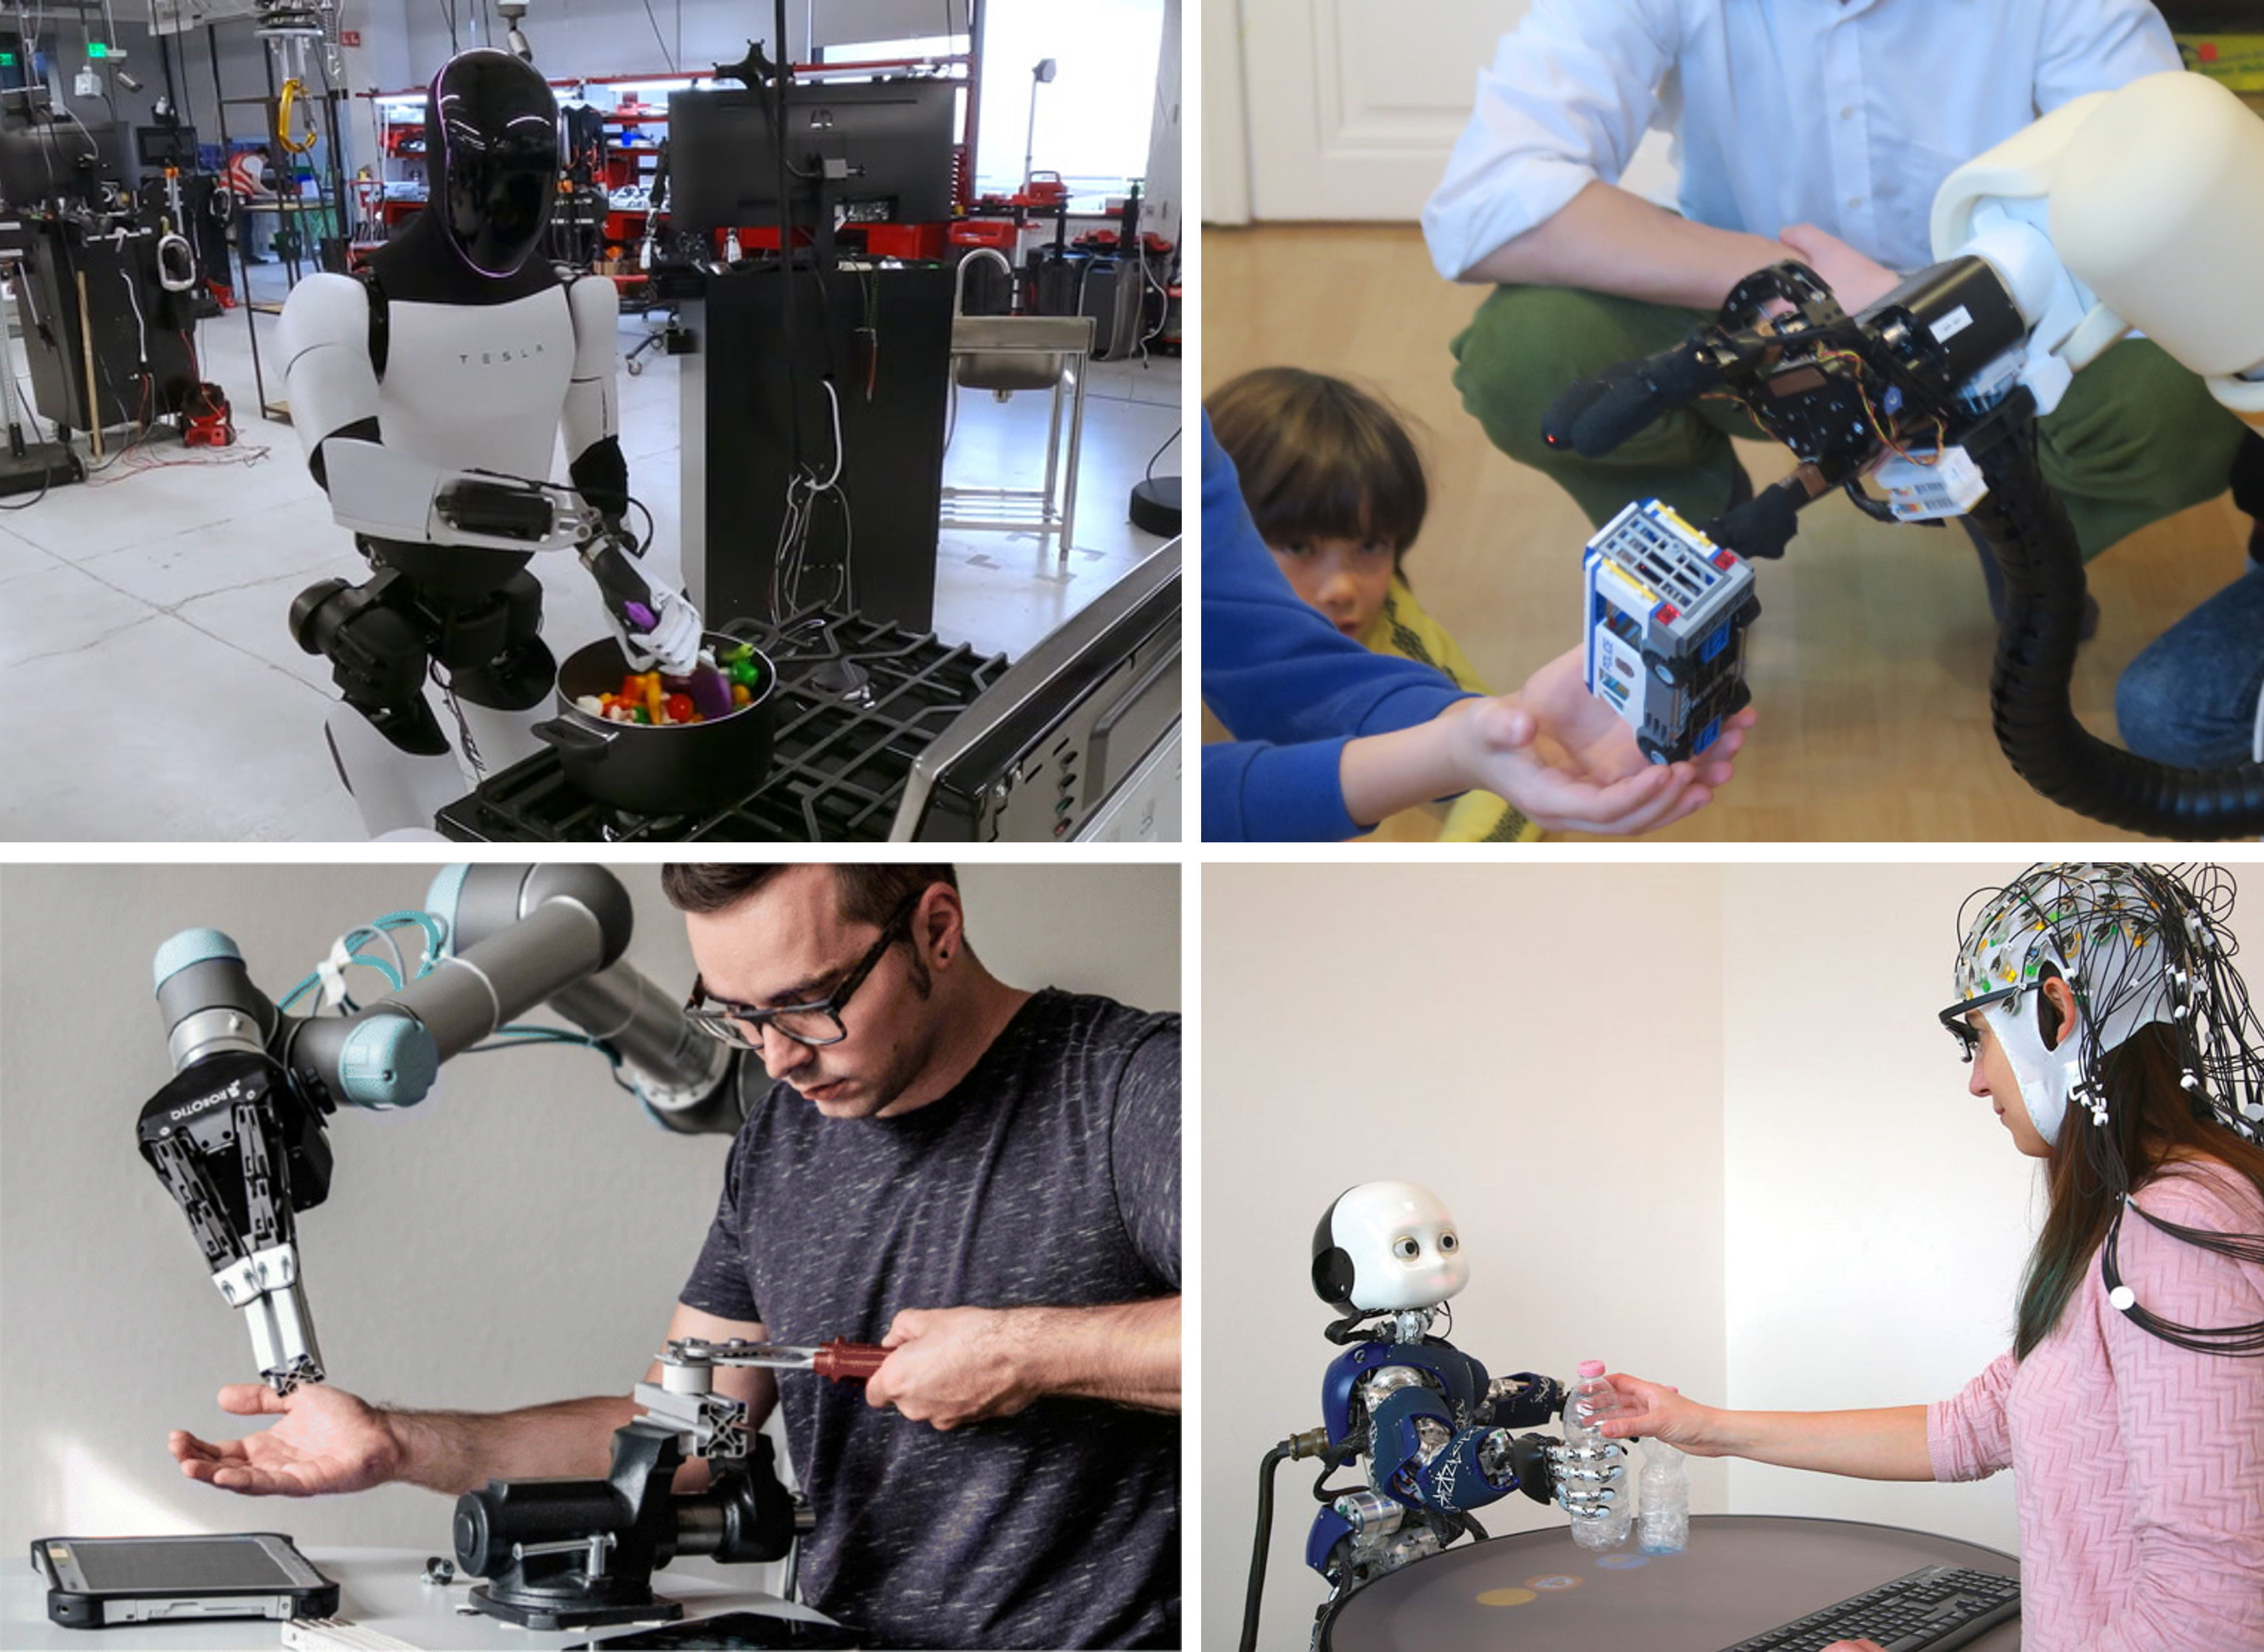
\includegraphics[width=0.8\textwidth]{general1}}
 	\caption{ورود ربات ها به دنیای تعامل با انسان ها
 		%\cite{kim2016integrated}
 	}
 	\label{fig:general1}
 \end{figure}


\section{نحوه‌ی ادراک  ربات ها از محیط و اشیاء}
ربات‌ها به طور معمول از حسگرهای گوناگونی برای درک محیط استفاده می‌کنند. این حسگرها را می‌توان به دو دسته  کلی غیرتماسی و تماسی تقسیم کرد. انواع دوربین های دوبعدی، تشخیص عمق و رادار لیزری
\LTRfootnote{LIDAR}
نمونه‌ای از حسگرهای غیرتماسی هستند که اطلاعاتی در مورد اشیاء و محیط، بدون تماس فیزیکی، فراهم می‌کنند. این حسگرها به در خدمت روش های یادگیری ماشین، توانسته‌اند ربات‌ها را قادر سازند تا برنامه‌ریزی صحیحی برای تعامل با محیط انجام دهند و محل مناسب برای گرفتن اشیاء را تشخیص دهند.
\cite{tian2023data,hosseini2024multi,beigy2024explorable,sabzejou20232d,moghadam2023grasp}
\subsection{آیا بینایی به تنهایی کافیست؟}

با وجود پیشرفت‌های چشمگیر در حوزه‌ی بینایی ماشین
\LTRfootnote{Computer Vision}
و کنترل ربات بر مبنای این حس
\LTRfootnote{Vision-based Robot Control}
،بینایی به تنهایی برای انجام وظایف پیچیده کافی نبوده و قادر به درک ویژگی‌های فیزیکی اشیا مانند نرمی، شکنندگی، بافت سطح یا نیروی اعمالی نیست. حس بینایی نمی‌تواند به طور مستقیم و در لحظه اصطکاک و یا لغزش بین چنگک و جسم را تشخیص دهد؛ با تکیه بر بینایی نمی‌توان میزان نیروی اعمال شده به یک جسم نرم یا شکننده را کنترل کرد.
\cite{yamaguchi2019recent,chi2018recent}
همچنین، هنگامی که چنگک
\LTRfootnote{Gripper}
 یک جسم را می‌گیرد، آن جسم ممکن است دید حسگر بینایی را مسدود کند و اطلاعات لحظه‌ای مربوط به تماس از دست برود. این ناتوانی‌ها چالشی بزرگ برای تعامل پایدار و مفید با اشیاء ایجاد می‌کنند. در نتیجه واضح است که صرفاً اتکا به حس بینایی برای انجام وظایف پیچیده و ظریف کافی نیست و نیاز به اطلاعات حسی دیگری به‌ خصوص حس لامسه ضروری است.
\subsection{لزوم حس لامسه در ربات}
حس لامسه یکی از مؤلفه‌های اصلی برای درک محیط توسط ربات، به‌ویژه در تعامل فیزیکی با اشیا، است. این حس امکان اندازه‌گیری نیروهای عمودی و جانبی، تشخیص برخورد با سایر عوامل موجود در محیط واعمال نیروی مناسب در حین انجام وظایف را فراهم می‌کند.
\cite{zou2017novel, yousef2011tactile}
وجود حس لامسه برای انجام وظایفی که نیازمند کنترل دقیق نیرو و تعامل ایمن با اشیای ظریف هستند، ضروری است. به عنوان مثال، در وظایف مونتاژ، جابه‌جایی مواد غذایی، یا تعامل با انسان، حس لامسه نقشی کلیدی در جلوگیری از آسیب به اشیا و بهبود عملکرد کلی ایفا می‌کند.
همچنین، پژوهش‌ها نشان داده‌اند که ادغام داده‌های لامسه و بینایی می‌تواند ادراک ربات را مشابه عملکرد انسان بهبود و سازگاری ربات با شرایط ناشناخته را افزایش دهد.
\cite{dahiya2013robotic}

\subsection{اهمیت حس لامسه در چنگک های رباتی}
عملگرهای نهایی 
\LTRfootnote{End-Effectors}
و به‌ویژه چنگک‌ها، اصلی‌ترین رابط مکانیکی بین ربات و محیط پیرامون آن محسوب می‌شوند. آن‌ها نقطه اصلی تماس ربات با اشیاء هستند و بخش عمده‌ای از وظایف یک ربات، از جمله گرفتن، جابجایی و دستکاری اشیاء، توسط این ابزارها انجام می‌شود. در دهه‌های گذشته، تمرکز اصلی در رباتیک صنعتی بر روی وظایف تکراری و از پیش تعریف‌‌شده در محیط‌های کاملاً کنترل‌شده بود؛ اما امروزه با گسترش کاربرد ربات‌ها در حوزه‌هایی مانند خدمات، پزشکی، کشاورزی و تعامل مستقیم با انسان، نیاز به ساختاری امن، قابل اعتماد و هوشمند برای این تعاملات به یکی از اهداف اصلی حوزه رباتیک تبدیل شده است.
\cite{broadbent2017interactions}
عملکرد قابل اطمینان برای چنگک‌های رباتی بسیار فراتر از یک گرفتن و رها کردن ساده است. یک گرفتن موفق نه تنها مستلزم لمس جسم هدف می‌باشد، بلکه باید از خطراتی مانند لغزش
\LTRfootnote{Slippage}
  شئ هدف و یا آسیب رساندن به آن به دلیل اعمال نیروی بیش از حد نیز جلوگیری شود. اینجاست که محدودیت‌های سیستم‌های کنترلی که صرفاً بر حس بینایی متکی هستند، آشکار می‌شود. اگرچه بینایی در مراحل اولیه مانند شناسایی و مکان‌یابی شیء نقشی حیاتی دارد، اما در لحظه تماس فیزیکی، به دلیل انسداد دید توسط خود چنگک و عدم توانایی درک خواص فیزیکی نامشهود، کارایی خود را از دست می‌دهد.
 \cite{malis2002survey}
 \\
 وجود حس لامسه در چنگک‌ها، این شکاف اطلاعاتی را پر کرده و کلید دستیابی به دستکاری 
 \LTRfootnote{Manipulation}
 پایدار، دقیق و هوشمند است. حسگرهای لامسه با فراهم آوردن اطلاعات بی‌درنگ از شرایط تماس، قابلیت‌های چنگک را به شکل چشمگیری افزایش می‌دهند. چند نوع از اطلاعاتی که حسگرهای لامسه می‌توانند فراهم کنند، شامل موارد زیر می‌شود:
 \begin{itemize}
 	\item \textbf{اندازه‌گیری نیرو و گشتاور } 
 	\\
حسگرهای لامسه می‌توانند مقادیر دقیق نیروهای نرمال و برشی اعمال‌شده بر سطح شیء را اندازه‌گیری کنند. این اطلاعات به سیستم کنترل اجازه می‌دهد تا نیروی گرفتن را به طور پیوسته تنظیم کند؛ نیروی اعمالی نباید آن‌قدر زیاد باشد که به جسم آسیب بزند و در عین حال، نباید آن‌قدر کم باشد که جسم بلغزد و از دست ربات رها شود
 	\cite{piga2023adaptive}
 	. توانایی انسان در بلند کردن یک تخم‌مرغ بدون شکستن آن، مثال بارزی از همین تنظیم دقیق نیرو بر اساس بازخورد لمسی است.
 	 
 	 \item \textbf{تشخیص لغزش} 
 	 \\
لغزش یکی از پدیده‌های دینامیکی کلیدی در حین دستکاری اشیاء است. حسگرهای لامسه، به‌ویژه آن‌هایی که به ارتعاشات فرکانس بالا حساس هستند، می‌توانند شروع لغزش را در مراحل اولیه تشخیص دهند. این تشخیص زودهنگام به کنترل‌کننده ربات فرصت می‌دهد تا به سرعت نیروی گرفتن را افزایش داده و از افتادن شیء جلوگیری کند.
 	 \cite{kyberd2023slip,costanzo2018slipping}
 	 
 	 \item \textbf{شناسایی موقعیت و توزیع تماس}
آرایه‌ای از حسگرهای لامسه می‌تواند نقشه‌ای از توزیع فشار بر روی سطح انگشتان چنگک ربات ایجاد کند. این اطلاعات برای تعیین مرکز فشار، تشخیص جهت‌گیری شیء در دست و اطمینان از یک گرفتن پایدار بسیار ارزشمند است.
\cite{khamis_novel_2019,de2022soft,wang_low-cost_2016}
\\
 \begin{figure}[ht]
	\centerline{\includegraphics[width=0.8\textwidth]{general2}}
	\caption{نمونه‌ای از تعامل چنگک های رباتی با اشیاء ظریف و نرم
		\cite{zhang2020state}
	}
	\label{fig:general1}
\end{figure}
 \end{itemize} 
\subsection{الهام از زیست: حس لامسه در انسان}
طبیعت در طول میلیون‌ها سال فرگشت، سیستم‌های بهینه‌ای را برای تعامل با محیط فیزیکی توسعه داده است. در میان این سیستم‌ها، حس لامسه انسان به عنوان پیچیده‌ترین، کارآمدترین و چندوجهی‌ترین سیستم حسی برای تعامل یا اشیاء شناخته می‌شود. پوست انسان، به‌ویژه در ناحیه نوک انگشتان، یک شاهکار مهندسی بیولوژیک است که ترکیبی از حساسیت بالا، استحکام، قابلیت ترمیم و توانایی پردازش اطلاعات پیچیده را به نمایش می‌گذارد. به همین دلیل، درک عمیق سازوکار حس لامسه انسان، نه تنها الهام‌بخش، بلکه یک نقشه راه ضروری برای طراحی و ساخت  حسگرهای رباتیکی است. 
\cite{silvera2015artificial}
موفقیت سیستم لامسه انسان در دستیابی به تعامل ماهرانه
\LTRfootnote{Dexterous Manipulation} 
 بر دو اصل بنیادین استوار است که در این پژوهش نیز به عنوان انگیزه اصلی مورد توجه قرار گرفته‌اند: 
 \textbf{اهمیت چندوجهی بودن ادراک حسی و ویژگی نرم و ارتجاعی نوک انگشتان.}
 در ادامه این بخش، این دو اصل کلیدی با جزئیات بیشتری بررسی می‌شوند.
\subsubsection{ ماهیت چندوجهی حس لامسه انسان}

پوست انسان یک حسگر یکپارچه و همگن نیست، بلکه مجموعه‌ای از گیرنده‌های حسی تخصصی است که هرکدام به نوع خاصی از محرک‌های لمسی با پهنای باند متفاوت پاسخ می‌دهند. این گیرنده‌های مکانیکی
 \LTRfootnote{Mechanoreceptors}
 که مسئول تبدیل محرک‌های لمسی به سیگنال‌های عصبی هستند، عمدتاً در لایه‌های روپوست
 \LTRfootnote{Epidermis}
و لایه‌ی میانی
\LTRfootnote{Dremis}
قرار دارند. در پوست بدون مو  مانند نوک انگشتان، که برای تعامل با اشیاء تکامل یافته‌اند، چهار نوع اصلی گیرنده مکانیکی وجود دارد که هر یک وظیفه مشخصی بر عهده دارند.
 \cite{wettels2011biomimetic, chi2018recent}.
\\
\begin{figure}[t]
	\centering
	\centerline{\includegraphics[width=0.8\textwidth]{Human_skin}}
	\caption{مقطعی از ساختار پوست انسان و محل قرارگیری چهار گیرنده لامسه اصلی در نوک انگشتان
		\cite{silvera2015artificial}
		. }
	\label{fig:skin_cross_section}
\end{figure}
این چهار گیرنده بر اساس سرعت پاسخشان به محرک‌های لامسه، به دو دسته اصلی تقسیم می‌شوند. دسته اول، گرینده های فرکانس پایین هستند که تا زمانی که محرک فیزیکی وجود داشته باشد، به طور پیوسته سیگنال عصبی تولید می‌کنند و مسئول درک اطلاعات استاتیک مانند نیرو هستند. دسته دوم، گیرنده های فرکانس بالا می‌باشند که فقط به تغییرات در محرک فیزیکی، یعنی در لحظه شروع و پایان تماس، پاسخ می‌دهند؛ این گروه مسئول درک اطلاعات دینامیک و گذرا هستند. این تقسیم‌بندی، اساس توانایی انسان در درک همزمان نیروهای مانا و پدیده‌های دینامیکی مانند لغزش است.
\begin{table}[ht]
	\caption{خلاصه‌ای از ویژگی‌ها و وظایف گیرنده‌های لامسه در نوک انگشتان انسان
\cite{chi2018recent}	
.}
	\label{tab:mechanoreceptors}
	\centering
	\onehalfspacing
	\begin{tabular}{|r|r|r|r|}
		\hline
		\textbf{نام گیرنده} & \textbf{محدوده فرکانس (هرتز)} &  \textbf{وظیفه اصلی} & \textbf{معادل در رباتیک} \\
		\hline \hline
		دیسک‌های مرکل
		\footnotemark
		
		 &  ۰.۳ - ۳ & فشار استاتیک&  نیروی گرفتن \\
		پایانه‌های رافینی
		\footnotemark
		 &  تا ۱۵ & کشش پوست، & نیروی مماسی\\
		گویچه‌های مایسنر
		\footnotemark
		 & ۳ - ۴۰ & تماس اولیه، لغزش آرام & تشخیص رویداد تماس \\
		گویچه‌های پاچینی 
		\footnotemark
		& ۱۰ - ۵۰۰ & ارتعاشات، لغزش  & تشخیص لغزش \\
		\hline
	\end{tabular}
\end{table}
\LTRfootnotetext[13]{Merkel's disks}
\LTRfootnotetext[14]{Ruffini's corpuscles}
\LTRfootnotetext[15]{Meissner corpuscles}
\LTRfootnotetext[16]{Pacinian corpuscles}
\\
این «تفکیک وجه ها» به مغز اجازه می‌دهد تا اطلاعات غنی و متنوعی را به صورت موازی پردازش کند و این همان اصلی است که این پژوهش با طراحی و ساخت یک حسگر چندوجهی
\LTRfootnote{Multi-modal}
قصد پایبندی به آن را دارد.
این تقسیم‌بندی پیچیده نشان می‌دهد که چرا تلاش برای ساخت یک حسگر لامسه رباتیک با تنها یک نوع تبدیل (مثلاً فقط اندازه‌گیری فشار) برای دستیابی به مهارت انسان کافی نیست. یک حسگر لامسه زیست الهام
\LTRfootnote{Biomimetic}
 واقعی باید بتواند اطلاعات استاتیک و دینامیک را در پهنای باندهای مختلف به صورت همزمان دریافت و پردازش کند
 \cite{silvera2015artificial}.
  این دقیقاً همان هدفی است که در این پژوهش با ترکیب یک حسگر فشار بارومتریک (برای درک اطلاعات استاتیک مشابه مرکل)، حسگرهای اثر هال (برای درک کشش و نیروی برشی مشابه رافینی)، حسگر دما و یک میکروفون (برای درک ارتعاشات فرکانس بالا مشابه پاچینی) دنبال شده است.


\subsubsection{ویژگی نرم و ارتجاعی نوک انگشتان}

دومین اصل کلیدی در موفقیت حس لامسه انسان، ماهیت فیزیکی خود انگشتان است. نوک انگشتان انسان از بافت نرم و ارتجاعی ساخته شده است که این ویژگی مزایای مکانیکی مهمی را در حین تعامل با اشیاء فراهم می‌کند.
یکی از مهم‌ترین این مزایا، \textbf{افزایش سطح تماس و پایداری گرفتن} است. هنگامی که یک انگشت نرم با یک جسم تماس پیدا می‌کند، تغییر شکل داده و خود را با شکل سطح جسم تطبیق می‌دهد. این امر باعث افزایش قابل توجه سطح تماس در مقایسه با یک انگشت صلب می‌شود. سطح تماس بزرگتر، نیروی گرفتن را بر روی ناحیه وسیع‌تری توزیع می‌کند که این امر اولاً خطر آسیب به اشیاء شکننده را کاهش می‌دهد و ثانیاً با افزایش مقاومت در برابر گشتاورهای خارجی، یک گرفتن بسیار پایدارتر ایجاد می‌کند
 \cite{yousef2011tactile}.

علاوه بر این، نرمی انگشتان بسیاری از عدم قطعیت‌ها و خطاهای کوچک در مکان‌یابی و جهت‌گیری شیء را جبران می‌کند. نیازی نیست که ربات موقعیت دقیق جسم را بداند؛ بافت نرم انگشت، خود را با ناهمواری‌ها و شکل‌های نامنظم تطبیق می‌دهد و یک تماس کامل را تضمین می‌کند. این ویژگی، نیاز به الگوریتم‌های کنترلی پیچیده را کاهش داده و به گرفتن قابل اطمینان کمک می‌کند.

نهایتاً، این تغییرشکل‌پذیری منجر به تقویت سیگنال‌های لمسی می‌شود. تغییر شکل پوست در اطراف یک شیء، الگوهای فشار و کشش منحصربه‌فردی را بر روی گیرنده‌های مکانیکی زیرین ایجاد می‌کند. به عنوان مثال، لبه‌های یک جسم باعث ایجاد تمرکز تنش در پوست می‌شوند که این امر به گیرنده‌های مرکل کمک می‌کند تا شکل را با دقت بیشتری تشخیص دهند. این پدیده به ربات نیز کمک می‌کند تا اطلاعات غنی‌تری از تماس استخراج کند.
\cite{silvera2015artificial}
این مزایا نشان می‌دهد که طراحی یک حسگر لامسه موفق، تنها به انتخاب مبدل‌های الکترونیکی مناسب محدود نمی‌شود، بلکه به طراحی مکانیکی و مواد به کار رفته در ساختار آن نیز بستگی دارد. استفاده از مواد نرم مانند سیلیکون در ساخت حسگرهای رباتیک، تلاشی برای تقلید از این ویژگی‌های سودمند فیزیکی انگشتان انسان است.

در نتیجه، با الهام از این دو اصل، این  پژوهش نه تنها بر توسعه یک سیستم الکترونیکی چندوجهی تمرکز داشته، بلکه این سیستم را در یک ساختار نرم و ارتجاعی ادغام می‌کند تا به ترکیبی بهینه از درک حسی و سازگاری مکانیکی، مشابه دست انسان، دست یابد.

\section{انواع روش های تبدیل در ساخت حسگر لامسه و مروری بر کار‌های پیشین}
\subsection{روش های مبتنی بر پیزوالکتریک}

از منظر لغوی، پیزو به معنی فشار است و ترکیب پیزو الکتریک
\LTRfootnote{Piezo-electric}
 به موادی اطلاق می‌شود که در اثر اعمال فشار، سیگنال الکتریکی از خود تولید می‌کنند. این حسگر‌ها از پدیده‌ای فیزیکی به نام اثر پیزوالکتریک بهره می‌برند. این اصطلاح علمی به معنای «الکتریسیته ناشی از فشار» است و به توانایی برخی مواد خاص برای تولید یک ولتاژ یا بار الکتریکی در پاسخ به کرنش مکانیکی یا فشار اشاره دارد. ساختار بلوری این مواد به گونه‌ای است که در حالت عادی، بارهای مثبت و منفی به طور متقارن توزیع شده و اثر یکدیگر را خنثی می‌کنند، اما با اعمال فشار یا نیروی مکانیکی، این تقارن به هم می‌خورد و بارهای الکتریکی مثبت و منفی در دو طرف ماده ظاهر می‌شوند، که منجر به تولید یک ولتاژ قابل اندازه‌گیری می‌گردد. این پدیده در موادی مانند کریستال‌های کوارتز 
\LTRfootnote{Quartz crystals}،
 سرامیک‌های پیزوالکتریک مانند PZT
 \LTRfootnote{Lead Zirconate Titanate}
  و برخی پلیمرها مانند PVDF
 \LTRfootnote{Polyvinylidene Fluoride}) مشاهده می‌شود.
\\
برای کاربردهای حسگر لامسه، مواد پیزوالکتریک به دلیل ویژگی‌های منحصربه‌فردشان بسیار مناسب هستند. این حسگرها نیازی به منبع تغذیه خارجی ندارند و می‌توانند به صورت فعال
\LTRfootnote{Active}
 عمل کنند که این ویژگی، مصرف انرژی را به شدت کاهش می‌دهد. مهم‌ترین مزیت این مکانیزم، پاسخ دینامیکی فوق‌العاده سریع و حساسیت بسیار بالا به تغییرات نیرو است. این خصوصیت آن‌ها را برای تشخیص ارتعاشات با فرکانس بالا و لغزش‌های بسیار جزئی
 \LTRfootnote{Micro-Slip}
 ایده‌آل می‌کند. در واقع، یک حسگر پیزوالکتریک می‌تواند لغزش یک جسم را در کسری از ثانیه تشخیص دهد که این امر به ربات اجازه می‌دهد قبل از افتادن کامل شیء، نیروی عمودی را اصلاح کند. پژوهش های متعددی در این زمینه انجام شده‌است که به ساخت حسگرهای لامسه پیزوالکتریک برای کاربردهای مختلف پرداخته‌اند. برای مثال، در پژوهش 
\cite{nasserii2011Piezo}
  نویسندگان به طراحی و ساخت یک حسگر بر اساس تغییر امپدانس کریستال پیزوالکتریک برای اندازه‌گیری نیروی اعمالی می‌پردازد. این حسگر با سنجش ولتاژ خروجی ناشی از فشار، توانایی تخمین نیروی اعمال شده را دارد. نتایج این پژوهش نشان داد که با توجه به طراحی ساده، حسگر ساخته شده قابلیت تغییر اندازه و شکل را دارد و برای کاربردهایی مانند جراحی‌های کم‌تهاجمی مناسب است. با این حال، جزئیات دقیق و کمی از دقت و حساسیت آن ارائه نشده است.
  همچنین،
  \cite{spanu2016PVDF}
   یک حسگر لمسی بسیار حساس را معرفی می‌کنند که از یک پلیمر پیزوالکتریک (PVDF) به همراه ترانزیستور ارگانیک استفاده می‌کند و برای پوست رباتیک مطرح شده است. حسگر مذکور توانایی اندازه‌گیری نیروهایی که به کوچکی 20mN را دارد.
   در مقاله‌ی 
   \cite{qi2023PVDF}
نویسندگان به بررسی انواع مواد قابل استفاده برای طراحی حسگر لامسه مبتنی بر پیزوالکتریک می‌پردازند.
    پژوهش‌هایی مانند
 \cite{wang2019PiezoArray,huang2024piezo,yu2016PiezoArray}
   به ساخت آرایه‌های حسگر پیزوالکتریک انعطاف‌پذیر برای اندازه‌گیری نیروهای سه‌محوری و تشخیص لغزش در حین گرفتن اشیاء پرداخته اند. سرعت خوانش اطلاعات در این پژوهش‌ها 5 تا 400 هرتز و در 
   \cite{huang2024piezo}
   1900 هرتز می‌باشد. بازه‌ی اندازه‌گیری نیرو به ترتیب 15، 11 و \LR{1.5} نیوتن برای محور عمودی گزارش شده است.
   
\begin{figure}[t]
	\centering
	\includegraphics[width=0.8\textwidth]{wang_piezo}
	\caption{شمای کلی حسگر ارائه شده در پژوهش 
		\cite{wang2019PiezoArray}
		. }
	\label{fig:wang_piezo}
\end{figure}
   
\begin{table}[ht]
	\centering
	\caption{مقایسه سنسورهای لمسی پیزوالکتریک گزارش‌شده در مقالات مختلف}
	\label{tab:piezo_sensors}
	\onehalfspacing
	\begin{tabular}{|r|r|r|r|r|r|}
		\hline
		\textbf{مرجع} & \textbf{سال} & \textbf{تعداد المان‌های حسی}  & \textbf{بازه نیرو} & \textbf{حساسیت} & \textbf{ماده پیزوالکتریک} \\ \hline \hline
		
		\cite{nasserii2011Piezo} & 2011 & 1 &$12 \: N$ & $33.47 \frac{mV}{N}$ & سرامیک پیزو \\ \hline
		
		\cite{spanu2016PVDF} & 2016 & 1 & 
		 $3.5 \: N$ & $3 \frac{nA}{N}$ & PVDF + Organic transistor \\ \hline
		
		\cite{yu2016PiezoArray} & 2016 & $2 \times 3 $ & $1.5 \: N$ & 
		$6.62 \frac{pC}{N}$ & \LR{PVDF} \\ \hline
		
		\cite{wang2019PiezoArray} & 2019 & $3 \times 3 $& $15 \: N$ &  $210 \frac{mV}{N}$ & PVDF \\ \hline
		
		\cite{huang2024piezo} & 2024 &$ 3‌ \times 3 $& $11 \: N$ & $35.6 \frac{mV}{N}$ & PVDF-based (rigid-in-soft) \\ \hline
		
	\end{tabular}
\end{table}

\subsection{روش های مبتنی بر پیزو مقاومت}
مکانیزم پیزومقاومتی یکی از بنیادی‌ترین و پرکاربردترین اصول در طراحی حسگرهای لامسه است که در سال‌های اخیر با توسعه مواد پیشرفته و ساختارهای میکرو و نانومتری توجه بسیاری را به خود جلب کرده است. اساس این روش بر این واقعیت استوار است که مقاومت الکتریکی یک ماده رسانا یا نیمه‌رسانا تحت تأثیر تغییرات مکانیکی نظیر فشار، کشش یا خمش تغییر می‌کند. این تغییر مقاومت را می‌توان به‌صورت یک سیگنال الکتریکی خواند و متناسب با آن شدت یا نوع تحریک مکانیکی را تعیین نمود. در واقع، تحریک مکانیکی به‌طور غیرمستقیم به یک پاسخ الکتریکی تبدیل می‌شود و همین امر امکان استفاده از آن را در ساخت پوست‌های مصنوعی، پروتزهای هوشمند و ربات‌های دارای قابلیت حس لامسه فراهم می‌سازد.

از دیدگاه فیزیکی، تغییرات مقاومت الکتریکی در یک ماده‌ی پیزو دو منشاء می‌تواند داشته باشد؛ منشاء اول تغییرات هندسی ماده مذکور است. همان‌طور که در رابطه‌ی کلاسیک مقاومت 
\begin{equation}\label{eq:piezoRes1}
	R=\rho\frac{l}{A}
\end{equation}
​

دیده می‌شود، اعمال تنش باعث افزایش طول و کاهش سطح مقطع یک رسانا می‌گردد و در نتیجه مقاومت آن تغییر می‌کند. دلیل دوم به تغییر مقاومت ویژه یا همان مقاومت ذاتی ماده مربوط است. در نیمه‌رساناهایی مانند سیلیکون و ژرمانیم، تنش مکانیکی موجب تغییر ساختار باند انرژی می‌شود و این تغییر، تحرک بارهای الکتریکی و چگالی آنها را دگرگون کرده و در نهایت مقاومت ویژه را تغییر می‌دهد
\begin{figure}[ht]
	\centering
	\includegraphics[width=0.8\textwidth]{piezoRes_ahmed2013mems}
	\caption{المان پیزومقاومتی استفاده شده در
		\cite{ahmed2013piezores}
		از جنس
		\LR{Si3N4 }}
		\label{fig:ahmed_piezores}
	\end{figure}
	. علاوه بر این دو منشاء، در ترکیباتی که شامل نانومواد کربنی، نانوسیم‌های فلزی یا ذرات رسانا هستند، تغییر مقاومت بیشتر ناشی از تغییر در مقاومت تماسی میان ذرات و پدیده‌هایی مانند تونل‌زنی کوانتومی
	\LTRfootnote{Quantum Tunneling Effect}
	است. زمانی که فشار به چنین ساختارهایی اعمال می‌شود، فاصله میان ذرات کاهش یافته و تماس‌های الکتریکی جدیدی ایجاد می‌شود که این فرایندها تغییرات شدیدی در مقاومت الکتریکی ایجاد می‌کنند.
	\cite{xi2024mechanisms}

	
	\begin{figure}[ht]
		\centering 
		\subfloat[مقوامت الکتریکی نسبت به نیرو\cite{drimus2014piezores}]{ \label{fig:pizeoResplots:RF}
			\includegraphics[width=0.5\textwidth]{drimus_2014_RF}}
		%\hspace{2mm}
		\subfloat[پسماند الکتریکی هنگام اعمال و برداشتن نیرو\cite{koiva2013piezores}]{ \label{fig:pizeoResplots:hysteresis}
			\includegraphics[width=0.5\textwidth]{koiva2013_piezoHysteresis}}%
		\caption{نمودارهای مشخصه برای حسگر های پیزومقاومتی.
		\ref{fig:pizeoResplots:RF}: مقاومت الکتریکی بر حسب نیرو.
	\ref{fig:pizeoResplots:hysteresis}پسماند سیگنال
\cite{koiva2013piezores}}
		\label{fig:pizeoResplots} %% label for entire figure
	\end{figure}
	
	
	
	پژوهش‌های متعددی برای بهبود حساسیت و محدوده‌ی عملکرد حسگرهای پیزومقاومتی انجام شده است. به عنوان نمونه، پژوهشگران در
	\cite{jing2022ag} 
	یک حسگر پیزومقاومتی انعطاف‌‌پذیر مبتنی بر نانوسیم‌های نقره و 
	\LR{PVDF}
	توسعه دادند که دارای ساختار سه‌بعدی متخلخل بود و به دلیل توزیع یکنواخت نانوسیم‌ها، حساسیت مناسبی در بازه ۰ تا ۱۰۰ کیلوپاسکال به دست آورد.  
	
	نمونه‌ی دیگر، پژوهش \cite{zhao2022pdms} است که از ترکیب نانولوله‌های کربنی و گرافن روی بستر
	\LR{PDMS}\LTRfootnote{Poly dimethyl siloxane}
	متخلخل استفاده کردند. آنها با ایجاد میکروحفره‌های یکنواخت در بستر از طریق گرمایش مایکروویوی، سطح تماس بسیار زیادی برای نانومواد رسانا فراهم آوردند. نتیجه این طراحی، دستیابی به حساسیتی در حدود \(300.31 \, kPa^{-1}\) در فشارهای پایین (۰ تا ۵۰ کیلوپاسکال) بود.  
	
	مکانیزم پیزومفاومتی محدودیت هایی نیز دارد؛ به طور مثال در شکل
	\ref{fig:pizeoResplots:RF}
	مشاهده می‌شود که رفتار غیرخطی حسگر در بازه‌های وسیع فشار باعث می‌شود رابطه بین نیروی واردشده و تغییر مقاومت همیشه خطی نبوده و کالیبراسیون دقیق را دشوار می‌سازد.
	علاوه بر این، با توجه به شکل 
	\ref{fig:pizeoResplots:hysteresis}
	وجود پسماند
	\LTRfootnote{Hysteresis}
	در پاسخ حسگر باعث می‌شود که مقادیر خروجی در هنگام اعمال و برداشت نیرو یکسان نباشد و دقت اندازه‌گیری کاهش یابد. عامل دیگر، حساسیت بالا به تغییرات دما است، زیرا افزایش دما می‌تواند تحرک حامل‌های بار و نیز مقاومت ویژه ماده را تغییر دهد و در نتیجه پاسخ حسگر را تحت تأثیر قرار دهد. همچنین این دسته از حسگرها اغلب دارای زمان بازیابی طولانی پس از اعمال نیرو هستند، به این معنا که بازگشت به حالت اولیه در بسیاری از طراحی‌ها به کندی صورت می‌گیرد. این ویژگی‌ها موجب محدودیت در استفاده از حسگرهای پیزومقاومتی در محیط‌هایی با تغییرات سریع نیرو یا دما شده و پژوهشگران را به سمت توسعه راهکارهای جبرانی، طراحی ترکیبی با مکانیزم‌های دیگر و استفاده از مواد نوین سوق داده است.
	
	
	\begin{table}[ht]
		\centering
		\caption{مقایسه سنسورهای لمسی پیزومقاومتی گزارش‌شده در مقالات مختلف}
		\label{tab:piezo_res}
		\onehalfspacing
		\begin{tabular}{|r|r|r|r|r|r|}
			\hline
			\textbf{مرجع} & \textbf{سال} & \textbf{تعداد المان‌های حسی}  & \textbf{بازه نیرو} & \textbf{حساسیت} & \textbf{ماده پیزوالکتریک} \\ \hline \hline
			
			\cite{noda2006cantilever} & 2006 & 1 &$-5 \: kPa - 5\: kPa (shear)$ & $0.03\%$ & Silicone \\ \hline
			
			\cite{koiva2013piezores} & 2013 & 12 & 
			$10 \: N$ & $0.015\%$ & LCPT\footnotemark \\ \hline
			
			\cite{ahmed2013piezores} & 2013 & $6 \times 8 $ & $30 \: kPa$ & 
			$1.25 \frac{V}{N}$ & \LR{Nichrome} \\ \hline
			
			\cite{drimus2014piezores} & 2014 & $8 \times 8 $ & $10 \: kPa$ & 
			$--$ & \LR{Conductive rubber} \\ \hline
			
			\cite{jing2022ag} & 2022 &$1$& $100 \: kPa$ &  $0.009 kPa^{-1} $ & AgNws + PVDF \\ \hline
			
			\cite{hou2022fiber} & 2022 &$ 1 $& $150 \: kPa$ & $2.06 kPa^{-1} $ & Cu + PDMS (rigid-in-soft) \\ \hline
			
			\cite{zhao2022pdms} & 2022 &$ 1$& $200 \: kPa$ & $300.31 kPa^{-1} $ & PDMS \\ \hline
		\end{tabular}
	\end{table}
	\LTRfootnote[30]{Liquid Crystal Polymer Thermoplastic}
	
\subsection{روش های خازنی}

فناوری خازنی یکی از پرکاربردترین و منعطف‌ترین رویکردها در طراحی حسگرهای لامسه رباتیک است. این حسگرها به دلیل حساسیت بالا، مصرف توان پایین و قابلیت مجتمع‌سازی در مقیاس بزرگ، توجه بسیاری از محققان را به خود جلب کرده‌اند. فلسفه اصلی در این حسگرها، اندازه‌گیری تغییر ظرفیت یک خازن بر اثر تغییر مکانیکی در ساختار و هندسه آن است. این حسگرها معمولاً از ساختاری شبیه به یک خازن صفحه‌موازی تشکیل شده‌اند که ظرفیت آن‌ها از طریق رابطه کلاسیک زیر محاسبه می‌شود:
\begin{equation}
	C=\frac{\varepsilon_0 \varepsilon_r A}{d}.
	\label{eq:basicC}
\end{equation}
در این رابطه، $C$ ظرفیت خازن، $\epsilon_0$ ثابت گذردهی خلأ، $\epsilon_r$ ثابت دی‌الکتریک نسبی ماده بین صفحات، $A$ سطح هم‌پوشانی صفحات و $d$ فاصله بین آن‌ها است. یک نیروی خارجی می‌تواند با تغییر پارامترهای هندسی \textbf{فاصله ($d$)} یا \textbf{سطح هم‌پوشانی ($A$)}، ظرفیت خازن را تغییر دهد و این تغییر، پس از اندازه‌گیری، به مقدار نیرو نگاشت می‌شود \cite{chi2018recent}.

اگرچه ساختار صفحه‌موازی اساس کار این حسگرهاست، اما طراحی‌های متنوعی برای اندازه‌گیری انواع مختلف نیرو (عمودی و برشی) و افزایش چشمگیر حساسیت توسعه یافته است.با این حال، متداول‌ترین مکانیزم، مبتنی بر \textbf{ساختار صفحه‌موازی برای نیروی عمودی} است. در این طراحی، یک لایه الاستومری نرم به عنوان ماده دی‌الکتریک بین دو الکترود رسانای انعطاف‌پذیر قرار می‌گیرد. هنگامی که یک نیروی عمودی به سطح حسگر وارد می‌شود، لایه الاستومری فشرده شده، فاصله $d$ بین صفحات کاهش می‌یابد و در نتیجه، ظرفیت خازن ($C$) به صورت غیرخطی افزایش پیدا می‌کند.

یک نوآوری کلیدی برای بهبود عملکرد این ساختار، استفاده از میکرو-ساختارها
\LTRfootnote{Micro-structures}
 در لایه دی‌الکتریک است. به جای استفاده از یک لایه صاف، الاستومر به شکل ساختارهای ریزی مانند هرم
\LTRfootnote{Pyramid}،
 گنبد 
 \LTRfootnote{Dome}
  یا ستون
  \LTRfootnote{Pillar}
   قالب‌گیری می‌شود \cite{mannsfeld2010highly}. این معماری هوشمندانه، نیرو را در نقاط کوچکی متمرکز کرده و باعث تغییر شکل بسیار بزرگتری در فاصله ($d$) به ازای یک فشار معین می‌شود. وجود فضاهای خالی در بین این میکرو-ساختارها باعث می‌شود حسگر در محدوده فشارهای پایین بسیار نرم و حساس عمل کند. در نتیجه، حساسیت حسگر فشار که به صورت زیر تعریف می‌شود:
  
  \begin{equation}
  	S = (\Delta C/C_0)/\Delta P
  	\label{eq:sensC}
  \end{equation}
     به شدت افزایش یافته و امکان تشخیص تماس‌های بسیار آرام را فراهم می‌آورد \cite{zou2017novel}.

علاوه بر روش ساخت، پیشرفت در علم مواد نیز تأثیر مستقیمی بر بهبود عملکرد، انعطاف‌پذیری و حساسیت حسگرهای خازنی داشته است. انتخاب لایه دی‌الکتریک نقشی حیاتی دارد؛ 
\LR{PDMS}
 به دلیل انعطاف ‌پذیری عالی، پایداری شیمیایی و زیست ‌سازگاری، یکی از محبوب‌ترین گزینه‌هاست. برای کاربردهایی که به نرمی بیشتری نیاز دارند، از الاستومرهایی مانند
 \LR{Ecoflex}
   نیز استفاده می‌شود. جهت افزایش بیشتر حساسیت، این پلیمرها گاهی با نانوذراتی با ثابت دی‌الکتریک بالا
 \LTRfootnote{High-k}
  مانند
  \LR{TiO₂} \LTRfootnote{Titanium dioxide}
    یا 
      \LR{BaTiO₃} \LTRfootnote{Barium titanate}
     ترکیب می‌شوند. این کار باعث افزایش ظرفیت اولیه خازن شده و تغییرات نسبی ظرفیت ($\Delta C/C_0$) را قابل توجه‌تر می‌سازد \cite{zou2017novel}.
     
برای آنکه کل حسگر انعطاف‌پذیر باشد، لایه‌های رسانا الکترودها نیز باید قابلیت تغییرشکل داشته باشند. به همین منظور، به جای لایه‌های فلزی صلب، از مواد رسانای انعطاف‌پذیر استفاده می‌شود. گزینه‌هایی مانند نانولوله‌های کربنی
\LTRfootnote{CNTs}، 
 گرافن
 \LTRfootnote{Graphene}، 
 پلیمرهای رسانا و حتی  فلز مایع مانند 
 \LR{EGaIn}\LTRfootnote{
 	Eutectic Gallium-Indium}
  به حسگر اجازه می‌ده دهند تا به راحتی خم شده و بر روی سطوح منحنی پیچیده‌ای مانند نوک انگشت  ربات نصب شوند \cite{chi2018recent}.


	\begin{figure}[t]
	\centering
	\includegraphics[width=0.8\textwidth]{capacitive1}
	\caption{ساختار حسگر لامسه خازنی معرفی شده در
		\cite{pagoli2022large}.}
	\label{fig:CapStructure}
\end{figure}

با وجود مزایای فراوان، طراحی و پیاده‌سازی حسگرهای خازنی با چالش‌های مهندسی خاصی روبروست. مهم‌ترین چالش‌ها، حساسیت به نویز و خازن پارازیتی است. این حسگرها به دلیل داشتن امپدانس خروجی بالا، به راحتی تحت تأثیر نویزهای الکترومغناطیسی
\LTRfootnote{EMI}
  محیط قرار می‌گیرند. علاوه بر این، خازن‌های ناخواسته (پارازیتی) که بین خطوط سیگنال و زمین شکل می‌گیرند، می‌توانند تغییرات کوچک ظرفیت اصلی حسگر را پوشانده و دقت اندازه‌گیری را کاهش دهند. برای مقابله با این مشکل از راهکارهایی مانند شیلدینگ فعال
   \LTRfootnote{Active Shielding}،
    که در آن یک الکترود محافظ هم‌پتانسیل با الکترود اصلی نویز را منحرف می‌کند، و طراحی‌های تفاضلی
    \LTRfootnote{Differential Sensing}،
  که با اندازه‌گیری تفاوت بین دو خازن نویز حالت مشترک را حذف می‌کند، استفاده می‌شود \cite{tiwana2012review}.

چالش دیگر، پدیده پسماند است که از ماهیت گرانروی کشسان 
\LTRfootnote{Viscoelasticity}
پلیمرهای دی‌الکتریک ناشی می‌شود. این پدیده باعث می‌شود منحنی پاسخ حسگر در هنگام افزایش نیرو با منحنی آن در هنگام کاهش نیرو یکسان نباشد و منجر به خطا در اندازه‌گیری شود. انتخاب مواد با پسماند ذاتی کمتر و اعمال چرخه‌های بارگذاری اولیه برای پایدارسازی رفتار ماده، از راهکارهای کاهش این اثر است.

نهایتاً، مدارهای اندازه‌گیری برای این حسگرها باید از پیچیدگی و دقت بالایی برخوردار باشند. از آنجایی که تغییرات ظرفیت اغلب در محدوده بسیار کوچک فمتوفاراد تا پیکوفاراد  است، مدارهای تخصصی برای تبدیل دقیق این تغییرات به سیگنال دیجیتال یا ولتاژ ضروری هستند. مبدل‌های ظرفیت به ولتاژ 
\LTRfootnote{C-V Converters}
 و مدارهای مبتنی بر نوسان‌ساز
\LTRfootnote{Oscillator-based circuits} 
از جمله معماری‌های رایج برای این منظور هستند.


\begin{table}[ht]
	\centering
	\caption{مقایسه سنسورهای لمسی خازنی گزارش ‌شده در مقالات مختلف}
	\label{tab:cap}
	\onehalfspacing
	\begin{tabular}{|r|r|r|r|r|r|}
		\hline
		\textbf{مرجع} & \textbf{سال} & \textbf{تعداد المان‌های حسی}  & \textbf{بازه نیرو} & \textbf{حساسیت} & \textbf{ماده دی‌الکتریک} \\ \hline \hline
		
		 \cite{castelli2002integrated} 
		& 2002 
		& $4 \times 4$ 
		& \LR{Tecnoflon FLOR 421} 
		& $81 \: N$
		& -- \\
		 \hline
		
		\cite{ulmen2010robust} 
		& 2010 
		& $4 \times 4$ 
		& \LR{Silicone} 
		&$100 \: N$ 
		& $20 mN $ \\
		 \hline
		
		\cite{chen2013friction} 
		& 2013 
		& $2 \times 2$ 
		& \LR{PDMS} 
		&$2 \: N$ 
		& $0.38 \frac{pF}{N}$ \\
		\hline
		
		\cite{wang2016three} 
		& 2017 
		& $3 \times 3$ 
		& \LR{PDMS} 
		&$10 \: N$ 
		& $0.369 \frac{V}{N}$ \\
		\hline
		
		\cite{pagoli2022large} & 2022 &$10 \times 10$& $2.5 \: N$ & $125 mN $ & PDMS \\ \hline
	\end{tabular}
\end{table}


\subsection{مکانیزم نوری}
حسگرهای لمسی نوری، از ویژگی‌های فیزیکی نور و یازتاب آن برای اندازه‌گیری نیرو یا تغییر شکل استفاده می‌کنند و یک رویکرد جذاب را در طراحی حسگرهای لمسی ارائه می‌دهند. این حسگرها با تبدیل تغییرات مکانیکی به تغییرات نوری، سیگنال قابل اندازه‌گیری ایجاد می‌کنند و به دلیل ماهیت خود، نسبت به تداخلات الکترومغناطیسی و نویزهای الکتریکی مقاوم هستند. در واقع، این حسگرها با استفاده از یک دوربین یا فتودیود، تغییر شکل یک سطح کشسان را در اثر تماس مشاهده می‌کنند. این روش امکان استخراج اطلاعات غنی از تماس، از جمله نیروی نرمال، نیروی مماسی، لغزش و حتی بافت سطح را فراهم می‌کند.
مکانیزم عملکرد این حسگرها عموماً بر پایه تغییر مسیر، شدت یا زاویه نور در پاسخ به یک نیروی خارجی استوار است. این حسگرها معمولاً از سه بخش اصلی تشکیل شده‌اند: یک منبع نور، یک بستر تغییر شکل‌پذیر و یک گیرنده نور. با اعمال نیرو به سطح حسگر، بستر تغییر شکل داده و نور را به گونه‌ای تغییر می‌دهد که با ثبت این تغییرات می‌توان میزان نیرو، جابه‌جایی یا حتی بافت جسم را اندازه‌گیری کرد. برای مثال، حسگر 
\LR{GelSight}
 که در 
\cite{yuan2017gelsight}
 معرفی شد و یکی از شناخته‌شده‌ترین نمونه‌های این مکانیزم است، از یک لایه کشسان و یک دوربین در زیر آن استفاده می‌کند تا تغییرات شکل سطح را در اثر تماس ثبت کند. پژوهش‌های مختلفی نیز با استفاده از تعداد محدودی حسگر حساس به نور اقدام به اندازه‌گیری نیرو کرده اند که در ادامه به آنها خواهیم پرداخت.به طور کلی، یکی از مهم‌ترین مزایای حسگرهای نوری، وضوح و دقت فضایی بسیار بالا است که به آن‌ها اجازه می‌دهد جزئیات بسیار دقیق تغییر شکل سطح را ثبت کنند. این ویژگی برای تشخیص بافت و شکل اشیا بسیار حیاتی است. علاوه بر این، این حسگرها به دلیل عدم نیاز به تماس الکتریکی با محیط، در برابر تداخلات الکترومغناطیسی و رطوبت مقاوم هستند. این مزیت، آن‌ها را برای کاربرد در محیط‌های صنعتی یا پزشکی که شرایط محیطی دشوار است، مناسب می‌سازد. از سوی دیگر، حسگرهای نوری معایبی نیز دارند. طراحی این حسگرها، به‌ویژه انواع مبتنی بر دوربین، می‌تواند پیچیده و حجیم باشد. همچنین، عملکرد آن‌ها به شدت به نور محیطی حساس است و ممکن است تحت تأثیر آن قرار گیرد، که نیاز به سیستم‌های محافظت در برابر نور را ایجاد می‌کند. در نهایت، ساخت این حسگرها، به خصوص نمونه‌های با رزولوشن بالا و سه‌محوری، ممکن است پرهزینه باشد. با این حال، با وجود این چالش‌ها، حسگرهای لمسی نوری به دلیل توانایی در ارائه اطلاعات غنی از تماس، به عنوان یک راه‌حل کلیدی در حوزه رباتیک و دستکاری اشیاء مطرح هستند.
\subsubsection{روش های مبتنی بر دوربین و ثبت تصویر کلی لامسه}

حسگرهای لمسی مبتنی بر دوربین، یک رویکرد نوین و قدرتمند در حوزه حسگرهای لمسی برای کاربردهای رباتیک ارائه می‌دهند. برخلاف حسگرهای سنتی که به اندازه‌گیری مستقیم نیرو می‌پردازند، این حسگرها از یک سیستم بینایی برای اندازه‌گیری هندسه و تغییر شکل سطح تماس استفاده می‌کنند. این روش به ربات امکان می‌دهد تا اطلاعات غنی و دقیقی از تماس را با وضوح فضایی بسیار بالا به دست آورد.
یکی از شناخته‌شده‌ترین و مهم‌ترین پژوهش‌ها در این دسته، توسعه حسگر لمسی نوری مبتنی بر بینایی با نام Gelsight است. مکانیزم عملکرد GelSight بر اساس اندازه‌گیری مستقیم تغییر شکل یک سطح الاستومری نرم است. این حسگر دارای یک سطح تماس شفاف و نرم است که با یک لایه از ذرات ریز براق (مانند پودر آلومینیوم) پوشانده شده است. یک منبع نور داخلی این سطح را روشن می‌کند و یک دوربین کوچک که در پشت حسگر قرار گرفته، تصویر آن را ثبت می‌کند.


زمانی که حسگر با یک جسم تماس پیدا می‌کند، سطح الاستومری تغییر شکل می‌دهد و خود را با هندسه دقیق جسم تطبیق می‌دهد. این تغییر شکل باعث تغییر در الگوی نور منعکس‌شده می‌شود. برآمدگی‌ها، ناهمواری‌ها و لبه‌های جسم باعث ایجاد سایه‌ها و تغییر در شدت نور می‌شوند. از طریق تحلیل تصویر ثبت‌شده توسط دوربین، می‌توان با استفاده از الگوریتم‌های پردازش تصویر، اطلاعات هندسی سطح تماس و همچنین اطلاعات مربوط به کشش روی سطح را استنباط کرد.
\begin{figure}[t]
	\centering
	\includegraphics[width=0.8\textwidth]{gelsight1}
	\caption{ساختار حسگر لامسه 
		\LR{Gelsight} معرفی شده در
		\cite{yuan2017gelsight}.}
	\label{fig:gelsight1}
\end{figure}

برخلاف حسگرهای لمسی سنتی که صرفاً نیروی تماس را اندازه‌گیری می‌کنند، GelSight قادر به اندازه‌گیری هندسه تماس با وضوح فضایی بسیار بالا است. این حسگر به طور همزمان می‌تواند تغییر شکل عمودی (فشار) و جانبی (کشش) را اندازه‌گیری کند. از این اطلاعات می‌توان برای استنباط نیروی تماس، گشتاور و لغزش استفاده کرد. توانایی این حسگر در درک دقیق شکل و بافت جسم، آن را برای وظایف پیچیده دستکاری، مانند گرفتن اشیاء با اشکال نامنظم یا بافت‌های ظریف، بسیار مناسب می‌سازد. با وجود مزایای متعدد حسگرهای لمسی مبتنی بر دوربین مانند GelSight در زمینه دقت و رزولوشن بالا، این سیستم‌ها با چالش‌ها و محدودیت‌هایی نیز روبرو هستند که استفاده از آن‌ها را در برخی شرایط خاص دشوار می‌سازد.
یکی از اصلی‌ترین معایب، حساسیت به نور محیطی است. از آنجا که عملکرد این حسگر به تحلیل تصویر نوری وابسته است، نورهای خارجی و محیطی (مانند نور خورشید یا چراغ‌های کارگاهی) می‌توانند بر روی الگوهای نوری ثبت‌شده توسط دوربین تأثیر گذاشته و در نتیجه دقت اندازه‌گیری را کاهش دهند. برای غلبه بر این مشکل، نیاز به طراحی‌های پیچیده برای محافظت در برابر نور محیط و استفاده از فیلترهای نوری خاص وجود دارد
\cite{li2015touching}.
دومین محدودیت مهم، پیچیدگی و حجم نسبی این حسگرها است. سیستم GelSight برای عملکرد خود نیازمند یک منبع نور داخلی، یک سطح الاستیک شفاف و یک دوربین با وضوح بالا است که همه در یک مجموعه فشرده قرار می‌گیرند. این نیاز به سخت‌افزارهای متعدد باعث می‌شود که حسگر حجم قابل توجهی داشته باشد، که می‌تواند آن را برای کاربرد در فضاهای محدود یا ربات‌های کوچک نامناسب سازد. علاوه بر این، هزینه ساخت این حسگرها، به‌ویژه به دلیل وجود قطعات نوری و الکترونیکی حساس و با کیفیت بالا، نسبت به حسگرهای لمسی ساده‌تر بالاتر است
\cite{dong2021high}.
از دیگر معایب می‌توان به آسیب‌پذیری سطح نرم حسگر اشاره کرد. سطح الاستیک و نرم GelSight، هرچند برای انطباق با اشکال مختلف ضروری است، اما در معرض خطراتی مانند سایش، بریدگی یا سوراخ شدن قرار دارد که می‌تواند به عملکرد حسگر آسیب برساند و نیاز به تعویض یا تعمیر داشته باشد. این امر دوام حسگر را در کاربردهای صنعتی سنگین کاهش می‌دهد
\cite{do2022densetact}.
در نهایت، نیاز به کالیبراسیون دقیق از دیگر معایب این روش است. برای تبدیل دقیق تغییرات پیکسل‌ها به مقادیر فیزیکی مانند نیرو و جابه‌جایی، نیاز به فرآیندهای کالیبراسیون پیچیده‌ای وجود دارد که می‌تواند زمان‌بر و دشوار باشد
\cite{yuan2017gelsight}.
\subsubsection{روش های مبتنی بر بازتاب نقطه ای نور}
متداول‌ترین روش استخراج اطلاعات لامسه، بهره بردن از مشخصات ارتجاعی و تغییر شکل یک سطح نرم می‎باشد. برای اندازه‌گیری مؤلفه‌های نیرو، می‎بایست این تغییر شکل به سیگنال های الکتریکی تبدیل شود. یکی از راه‌های رسیدن به این امر استفاده از نور مادون قرمز است. به طوری که بازتاب نور در اثر تغییر شکل سطح ارتجاعی تغییر می‎کند و با بررسی نور بازتاب‌ شده می‌توان نوع تغییر شکل را تشخیص داد. در راستای این روش پژوهش های بسیاری انجام شده که اغلب موفق بوده و به محصولاتی تجاری ختم شده‌اند. یکی از این روش ها در 
\cite{khamis_novel_2019}
ارائه شده است. در این پژوهش یک طراحی جدید دوربین سوراخ سوزنی
\LTRfootnote{Pin-hole camera}
 اجرا شده‌است که در اصل یک فوتودیود چهارتایی
 \LTRfootnote{Quadrant Photo Diode (QPD)}
  بوده و تغییر شکل قسمت کشسان منجر به حرکت و تغییر در ناحیه یک نقطه نوری می شود که بر روی این فتودیود چهارتایی پخش می شود. سیگنال‌های چهار فوتودیود با استفاده از رگرسیون چند متغیره به جابجایی و نیروی سه بعدی واقعی نگاشت می شوند. 
  \begin{figure}[t]
  	\centering
  	\includegraphics[width=0.8\textwidth]{optical_khamis}
  	\caption{ساختار حسگر لامسه مبتنی بر بازتاب نور
  		\cite{khamis_novel_2019}.}
  	\label{fig:optical_khamis}
  \end{figure}
این روش دارای مزایای قابل توجهی است که آن را از بسیاری از طراحی‌های دیگر متمایز می‌کند. مهم‌ترین نقطه قوت آن، توانایی ذاتی در اندازه‌گیری بردار کامل نیروی سه‌بعدی، شامل نیروهای عمودی و برشی، در هر المان
\LTRfootnote{Taxel}
 به صورت مجزا است. این قابلیت، اطلاعات بسیار غنی‌تری را در مقایسه با حسگرهای فشار ساده فراهم می‌کند. علاوه بر این، حساسیت بالای آن به ارتعاشات سریع، این حسگر را به یک گزینه ایده‌آل برای کاربردهای پیشرفته‌ای مانند تشخیص لغزش تبدیل کرده است. د

با این وجود، این طراحی با چالش‌ها و معایبی نیز همراه است. پیچیدگی ساختاری هر المان، که شامل اجزای متعدد نوری و مکانیکی است، فرآیند ساخت و مونتاژ آن را در مقایسه با حسگرهای ساده‌تر مانند خازنی یا مقاومتی، دشوارتر و پرهزینه‌تر می‌کند. چالش دیگر، نیاز به یک فرآیند کالیبراسیون پیچیده است؛ نگاشت سیگنال‌های دریافتی از چهار بخش فوتودیود به یک بردار نیروی سه‌بعدی، یک رابطه خطی ساده نیست و نیازمند استفاده از روش‌های رگرسیون چندمتغیره برای هر حسگر به صورت جداگانه است. در نهایت، مانند سایر سیستم‌های نوری، این حسگر نیز می‌تواند به تداخل نوری از منابع خارجی حساس باشد و برای عملکرد صحیح نیازمند آب‌بندی دقیق در برابر نور محیط است.
\cite{khamis_novel_2019}
روش دیگری نیز مشابه این کار در پژوهش 
\cite{costanzo2021optical}
 معرفی شده است.طراحی ارائه شده در این پژوهش اساساً از یک ساختار دو لایه تشکیل شده است. لایه اول، لایه اپتوالکترونیک 
 \LTRfootnote{Optoelectronic}
   است که معمولاً یک برد مدار چاپی صلب بوده و تمام قطعات الکترونیکی روی آن نصب می‌شوند. برای هرالمان حسی، این لایه شامل یک جفت قطعه اپتوالکترونیک است: یک منبع نور که به شکل دیود ساطع‌کننده نور مادون قرمز می‌باشد و یک آشکارساز نور که معمولاً یک ترانزیستور نوری
   \LTRfootnote{Phototransistor}
    یا فوتودیود است و وظیفه دریافت نور بازتاب‌شده را بر عهده دارد.
 لایه دوم، لایه ارتجاعی و کشسان است که مستقیماً با اشیاء خارجی تماس پیدا می‌کند و از یک ماده نرم و ارتجاعی مانند سیلیکون ساخته می‌شود. این لایه دارای ویژگی‌های طراحی هوشمندانه‌ای است؛ بدنه اصلی آن از سیلیکون به رنگ سیاه ساخته شده است تا هم از ورود نور محیط به داخل حسگر و ایجاد اختلال جلوگیری کند و هم از تداخل نوری
  \LTRfootnote{Crosstalk}
   بین المان‌های مجاور ممانعت به عمل آورد. در مقابل، سطحی از لایه سیلیکون که رو به قطعات اپتوالکترونیک قرار دارد، به رنگ سفید پوشانده می‌شود. این سطح سفید، نور مادون قرمز تابیده‌شده از LED را به طور مؤثری به سمت فتوتزانزیستور بازتاب می‌دهد که این امر منجر به افزایش چشمگیر حساسیت حسگر می‌شود.
\\
 فرآیند اندازه‌گیری نیرو در این حسگر به این صورت است که در حالت بدون نیرو، منبع مادون قرمز نور را به سطح سفید داخلی لایه سیلیکون می‌تاباند. از آنجایی که سطح در فاصله مشخصی قرار دارد، مقدار معینی از نور بازتاب شده و توسط فوتوترانزیستور دریافت می‌شود که این امر یک خروجی ولتاژ پایه را در حسگر ایجاد می‌کند. با اعمال یک نیروی خارجی به سطح حسگر، لایه سیلیکونی نرم فشرده شده و تغییر شکل می‌دهد. این تغییر شکل باعث می‌شود که سطح سفید بازتابنده به منبع نور و آشکارساز نزدیک‌تر شود. این کاهش فاصله، شدت نور بازتابی را افزایش می‌دهد، زیرا نور کمتری در مسیر بازگشت پراکنده شده و مقدار بیشتری از آن به آشکارساز می‌رسد. فوتوترانزیستور این افزایش شدت نور را به یک جریان الکتریکی بزرگتر و در نهایت به یک سیگنال ولتاژ بالاتر تبدیل می‌کند. در نتیجه، ولتاژ خروجی حسگر مستقیماً با میزان تغییر شکل و در نهایت، با نیروی اعمال‌شده متناسب خواهد بود. با چیدن این المان‌ها در کنار یکدیگر به صورت یک آرایه، می‌توان یک نقشه از توزیع فشار بر روی سطح حسگر ایجاد کرد
 \cite{costanzo2021optical}.
 با این وجود، ایرادات معمول وارد بر روش های مشابه مبتنی بر نور، در این پژوهش نیز مشاهده می‌شود، مانند دقت پایین و حساسیت به نور محیط.
 \begin{table}[ht]
 	\centering
 	\caption{مقایسه سنسورهای لمسی خازنی گزارش ‌شده در مقالات مختلف}
 	\label{tab:cap}
 	\onehalfspacing
 	\begin{tabular}{|r|r|r|r|r|}
 		\hline
 		\textbf{مرجع} & \textbf{سال}  & \textbf{بازه نیرو} & \textbf{حساسیت} & \textbf{نوع حسگر نوری} \\ \hline \hline
 		Yuan et al. (GelSight) \cite{yuan_gelsight_2017} & 2017 & تک‌المان (پیکسل‌های تصویری) & تا حدود 10 N & دقت زیر 0.1 N، رزولوشن میکرونی \\ \hline
 		Khamis et al. (PapillArray) \cite{khamis_novel_2019} & 2019 & آرایه 16 تایی پاپیلا & 0 -- 8 N & $\approx$0.01 N \\ \hline
 		Costanzo \& Pirozzi \cite{costanzo_optical_2021} & 2021 & تک‌المان (فیبر نوری و بازتاب نور) & 0 -- 15 N & دقت نیرو $\pm$0.1 N \\ \hline
 		Do et al. (DenseTact 2.0) \cite{do_densetact_2023} & 2023 & تک‌المان با پوشش وسیع تصویری & 0 -- 20 N & دقت نیرو $\pm$0.1 N، دقت شکل $\sim 50 \mu m$ \\ \hline
 		Kara et al. (QS-TS) \cite{kara_towards_2023} & 2023 & تک‌المان (ArUco markers) & تا 5 N & خطای کمتر از 5\% \\ \hline
 		Leslie et al. (3D Force Sensor) \cite{leslie_tactile_2023} & 2023 & تک‌المان (زاویه نور) & 0 -- 10 N & دقت نیرو $\pm$0.05 N \\ \hline
 		\cite{yuan2017gelsight} 
 		& 2017 
 		& $10 \: N$
 		& $100 \: mN$
 		&دوربین\\
 		\hline
 		
 		\cite{khamis_novel_2019} 
 		& 2019
 		& $11 \: N$
 		& $190 \: mN$
 		&فوتودیود چهارتایی\\
 		\hline
 		
 		\cite{costanzo2021optical} 
 		& 2021
 		& $15 \: N$
 		& $100 \: mN$
 		&فوتودیود \\
 		\hline
 		
 		\cite{do2022densetact} 
 		& 2023
 		& $20 \: N$
 		& $100 \: mN$
 		&دوربین\\
 		\hline
 		
 		\cite{kara2023towards} 
 		& 2023
 		& $5 \: N$
 		& $5 \%$
 		&دوربین\\
 		\hline
 		
 		\cite{leslie2023tactile} 
 		& 2023
 		& $10 \: N$
 		& $iuykjthrgf$
 		&دوربین\\
 		\hline
 	\end{tabular}
 \end{table}
\subsubsection{نوشتن فصل‌ها}
همان‌طور که در بخش \ref{muchFiles} گفته شد برای جلوگیری از شلوغی، قسمت‌های مختلف \پ از جمله فصل‌ها، در فایل‌های جداگانه‌ای قرار داده شده‌اند. 
مثلاً اگر می‌خواهید مطالب فصل ۱ را تایپ کنید، باید فایل‌های 
\lr{main.tex}
و
\lr{chapter1.tex}
را باز کرده و مطالب خود را جایگزین محتویات داخل 
\lr{chapter1.tex}
نمایید. دقت شود که در ابتدای برخی فایلها دستوراتی نوشته شده است و از شما خواسته شده که آن دستورات را حذف نکنید.

%توجه کنید که همان‌طور که قبلاً هم گفته شد، تنها فایل قابل اجرا، 
%\lr{main.tex}
%است. لذا برای دیدن حاصل (خروجی) فایل خود، باید  
%\lr{chapter1.tex}
%را ذخیره کرده و سپس فایل 
%\lr{main.tex}
%را اجرا کنید.

نکته بسیار مهمی که در اینجا باید گفته شود این است که سیستم \lr{\TeX}، محتویات یک فایل تِک را به ترتیب پردازش می‌کند.  بنابراین، اگر مثلاً  دو فصل اول خود را نوشته و خروجی آنها را دیده‌اید و مشغول تایپ مطالب فصل ۳ هستید، بهتر است
که دو دستور 
\verb!% !TeX root=../main.tex

\chapter{مقدمه}
% دستور زیر باعث عدم‌نمایش شماره صفحه در اولین صفحهٔ این فصل می‌شود.
%\thispagestyle{empty}
\section{پیشگفتار}
رباتیک حوزه‌ای میان‌رشته‌ای متشکل از دانش مکانیک، الکترونیک، کنترل و علوم رایانه می‌باشد که به طراحی، ساخت و بهره‌برداری از سامانه‌هایی می‌پردازد که قادرند وظایف را به‌صورت خودکار یا نیمه‌خودکار انجام دهند.
\cite{wallen2008history}
 از دهه ها قبل، ورود ربات‌ها به صنایع، آن‌ها را به عنوان راه‌حل‌هایی قابل اعتماد، دقیق و خستگی‌ناپذیر برای صنعتگران تثبیت کرده است. با پیشرفت روزافزون فناوری، کاهش هزینه‌های تولید، کاربرد ربات‌ها از محیط‌های صنعتی کنترل‌شده فراتر رفته و پا بر عرصه‌ تعامل مستقیم با انسان‌ها در محیط‌های اجتماعی و خانگی گذاشت. 
 \cite{broadbent2017interactions,dahiya2013robotic}
 در ادامه‌ی این گسترش کاربر و با رشد هوش مصنوعی، یادگیری ماشین و حسگرهای پیشرفته، علم رباتیک در حوزه های پزشکی، کشاورزی، خدمات، اکتشاف و تعامل اجتماعی با انسان نیز ورود کرده است.
 \cite{wang2024multimodal,sheridan2016human}
  این گسترشِ دامنهٔ کاربرد، اهمیت درک عمیق‌تر ربات از محیط و تعامل ایمن و با انسان و اشیاء را بیش از پیش برجسته کرده است. برای رسیدن به مهم، ربات‌ها باید قادر باشند محیط خود را بفهمند و با اشیاء و محیط به شیوه‌ای مشابه انسان‌ها تعامل کنند. در نتیجه، برای گذار از ربات های صرفاً تکرارکار به ربات ‌های هوشمند و تطبیق‌پذیر، طراحی و ساخت حسگرهای پیشرفته و چندوجهی
  \LTRfootnote{Multi-modal}
  بهره بردن حداکثری از داده های آن‌ها ضرورت دارد.
  \cite{wang2024multimodal}
  \\
 \begin{figure}[ht]
 	\centerline{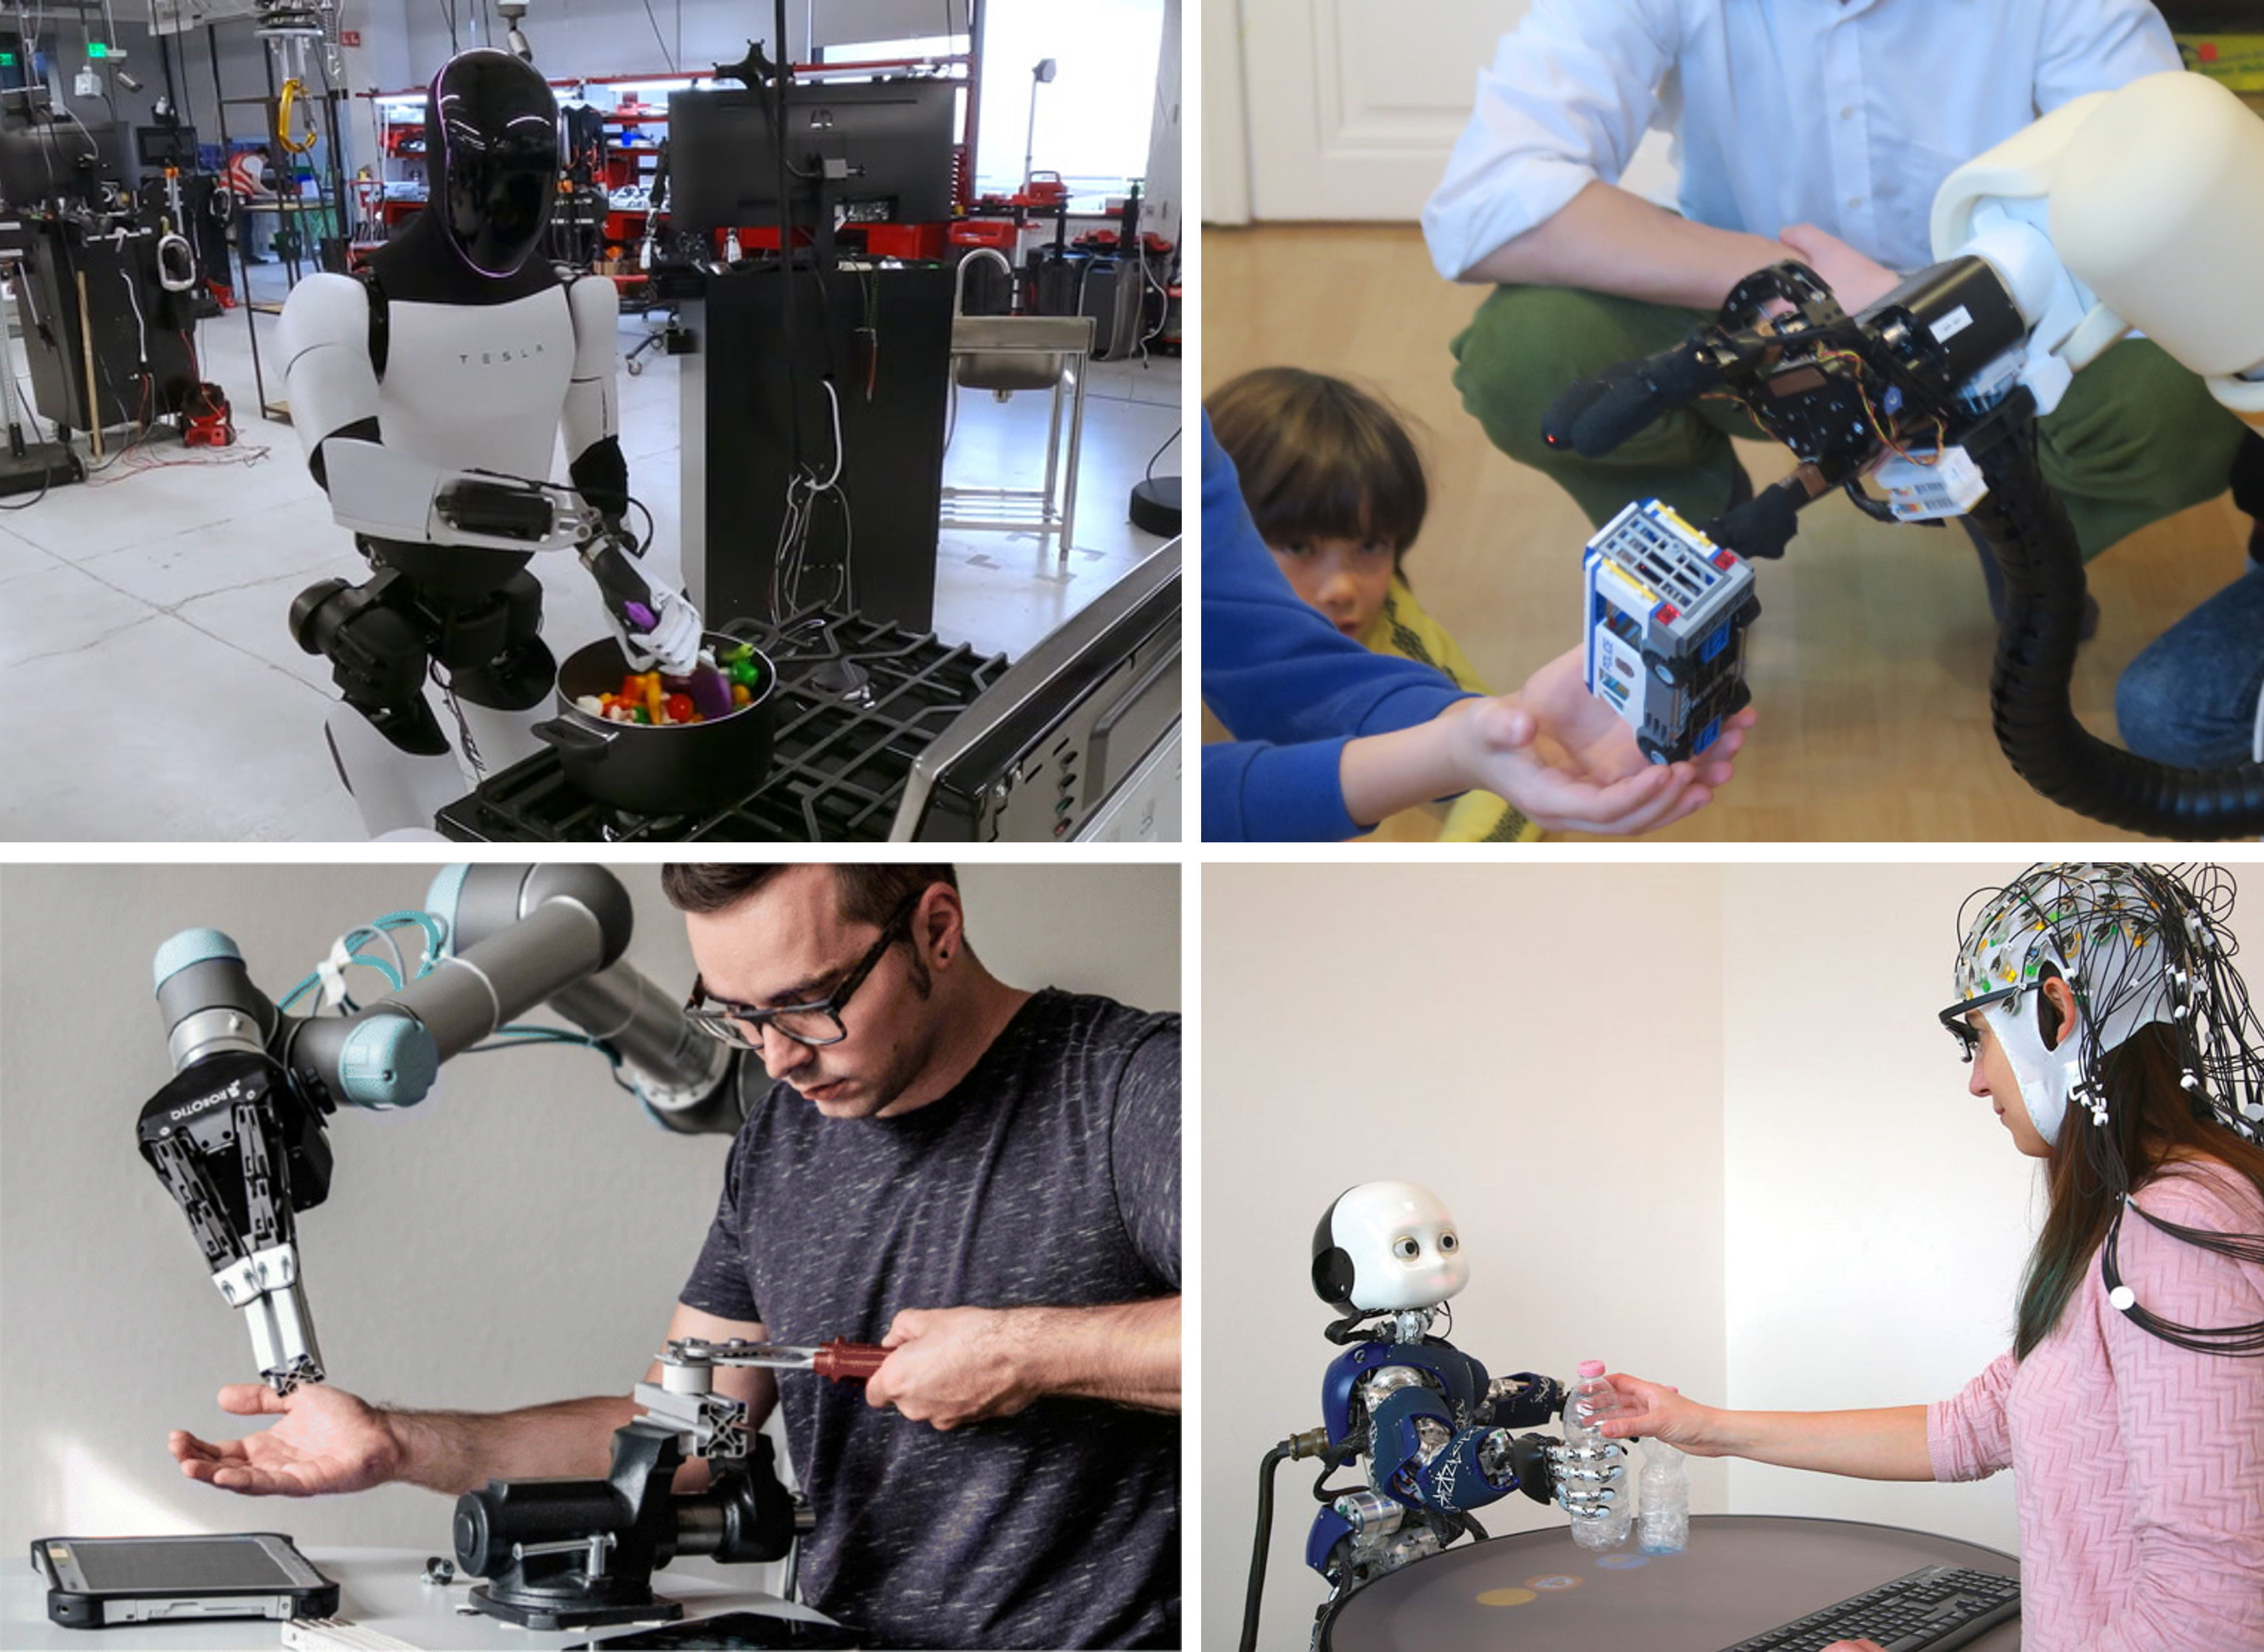
\includegraphics[width=0.8\textwidth]{general1}}
 	\caption{ورود ربات ها به دنیای تعامل با انسان ها
 		%\cite{kim2016integrated}
 	}
 	\label{fig:general1}
 \end{figure}


\section{نحوه‌ی ادراک  ربات ها از محیط و اشیاء}
ربات‌ها به طور معمول از حسگرهای گوناگونی برای درک محیط استفاده می‌کنند. این حسگرها را می‌توان به دو دسته  کلی غیرتماسی و تماسی تقسیم کرد. انواع دوربین های دوبعدی، تشخیص عمق و رادار لیزری
\LTRfootnote{LIDAR}
نمونه‌ای از حسگرهای غیرتماسی هستند که اطلاعاتی در مورد اشیاء و محیط، بدون تماس فیزیکی، فراهم می‌کنند. این حسگرها به در خدمت روش های یادگیری ماشین، توانسته‌اند ربات‌ها را قادر سازند تا برنامه‌ریزی صحیحی برای تعامل با محیط انجام دهند و محل مناسب برای گرفتن اشیاء را تشخیص دهند.
\cite{tian2023data,hosseini2024multi,beigy2024explorable,sabzejou20232d,moghadam2023grasp}
\subsection{آیا بینایی به تنهایی کافیست؟}

با وجود پیشرفت‌های چشمگیر در حوزه‌ی بینایی ماشین
\LTRfootnote{Computer Vision}
و کنترل ربات بر مبنای این حس
\LTRfootnote{Vision-based Robot Control}
،بینایی به تنهایی برای انجام وظایف پیچیده کافی نبوده و قادر به درک ویژگی‌های فیزیکی اشیا مانند نرمی، شکنندگی، بافت سطح یا نیروی اعمالی نیست. حس بینایی نمی‌تواند به طور مستقیم و در لحظه اصطکاک و یا لغزش بین چنگک و جسم را تشخیص دهد؛ با تکیه بر بینایی نمی‌توان میزان نیروی اعمال شده به یک جسم نرم یا شکننده را کنترل کرد.
\cite{yamaguchi2019recent,chi2018recent}
همچنین، هنگامی که چنگک
\LTRfootnote{Gripper}
 یک جسم را می‌گیرد، آن جسم ممکن است دید حسگر بینایی را مسدود کند و اطلاعات لحظه‌ای مربوط به تماس از دست برود. این ناتوانی‌ها چالشی بزرگ برای تعامل پایدار و مفید با اشیاء ایجاد می‌کنند. در نتیجه واضح است که صرفاً اتکا به حس بینایی برای انجام وظایف پیچیده و ظریف کافی نیست و نیاز به اطلاعات حسی دیگری به‌ خصوص حس لامسه ضروری است.
\subsection{لزوم حس لامسه در ربات}
حس لامسه یکی از مؤلفه‌های اصلی برای درک محیط توسط ربات، به‌ویژه در تعامل فیزیکی با اشیا، است. این حس امکان اندازه‌گیری نیروهای عمودی و جانبی، تشخیص برخورد با سایر عوامل موجود در محیط واعمال نیروی مناسب در حین انجام وظایف را فراهم می‌کند.
\cite{zou2017novel, yousef2011tactile}
وجود حس لامسه برای انجام وظایفی که نیازمند کنترل دقیق نیرو و تعامل ایمن با اشیای ظریف هستند، ضروری است. به عنوان مثال، در وظایف مونتاژ، جابه‌جایی مواد غذایی، یا تعامل با انسان، حس لامسه نقشی کلیدی در جلوگیری از آسیب به اشیا و بهبود عملکرد کلی ایفا می‌کند.
همچنین، پژوهش‌ها نشان داده‌اند که ادغام داده‌های لامسه و بینایی می‌تواند ادراک ربات را مشابه عملکرد انسان بهبود و سازگاری ربات با شرایط ناشناخته را افزایش دهد.
\cite{dahiya2013robotic}

\subsection{اهمیت حس لامسه در چنگک های رباتی}
عملگرهای نهایی 
\LTRfootnote{End-Effectors}
و به‌ویژه چنگک‌ها، اصلی‌ترین رابط مکانیکی بین ربات و محیط پیرامون آن محسوب می‌شوند. آن‌ها نقطه اصلی تماس ربات با اشیاء هستند و بخش عمده‌ای از وظایف یک ربات، از جمله گرفتن، جابجایی و دستکاری اشیاء، توسط این ابزارها انجام می‌شود. در دهه‌های گذشته، تمرکز اصلی در رباتیک صنعتی بر روی وظایف تکراری و از پیش تعریف‌‌شده در محیط‌های کاملاً کنترل‌شده بود؛ اما امروزه با گسترش کاربرد ربات‌ها در حوزه‌هایی مانند خدمات، پزشکی، کشاورزی و تعامل مستقیم با انسان، نیاز به ساختاری امن، قابل اعتماد و هوشمند برای این تعاملات به یکی از اهداف اصلی حوزه رباتیک تبدیل شده است.
\cite{broadbent2017interactions}
عملکرد قابل اطمینان برای چنگک‌های رباتی بسیار فراتر از یک گرفتن و رها کردن ساده است. یک گرفتن موفق نه تنها مستلزم لمس جسم هدف می‌باشد، بلکه باید از خطراتی مانند لغزش
\LTRfootnote{Slippage}
  شئ هدف و یا آسیب رساندن به آن به دلیل اعمال نیروی بیش از حد نیز جلوگیری شود. اینجاست که محدودیت‌های سیستم‌های کنترلی که صرفاً بر حس بینایی متکی هستند، آشکار می‌شود. اگرچه بینایی در مراحل اولیه مانند شناسایی و مکان‌یابی شیء نقشی حیاتی دارد، اما در لحظه تماس فیزیکی، به دلیل انسداد دید توسط خود چنگک و عدم توانایی درک خواص فیزیکی نامشهود، کارایی خود را از دست می‌دهد.
 \cite{malis2002survey}
 \\
 وجود حس لامسه در چنگک‌ها، این شکاف اطلاعاتی را پر کرده و کلید دستیابی به دستکاری 
 \LTRfootnote{Manipulation}
 پایدار، دقیق و هوشمند است. حسگرهای لامسه با فراهم آوردن اطلاعات بی‌درنگ از شرایط تماس، قابلیت‌های چنگک را به شکل چشمگیری افزایش می‌دهند. چند نوع از اطلاعاتی که حسگرهای لامسه می‌توانند فراهم کنند، شامل موارد زیر می‌شود:
 \begin{itemize}
 	\item \textbf{اندازه‌گیری نیرو و گشتاور } 
 	\\
حسگرهای لامسه می‌توانند مقادیر دقیق نیروهای نرمال و برشی اعمال‌شده بر سطح شیء را اندازه‌گیری کنند. این اطلاعات به سیستم کنترل اجازه می‌دهد تا نیروی گرفتن را به طور پیوسته تنظیم کند؛ نیروی اعمالی نباید آن‌قدر زیاد باشد که به جسم آسیب بزند و در عین حال، نباید آن‌قدر کم باشد که جسم بلغزد و از دست ربات رها شود
 	\cite{piga2023adaptive}
 	. توانایی انسان در بلند کردن یک تخم‌مرغ بدون شکستن آن، مثال بارزی از همین تنظیم دقیق نیرو بر اساس بازخورد لمسی است.
 	 
 	 \item \textbf{تشخیص لغزش} 
 	 \\
لغزش یکی از پدیده‌های دینامیکی کلیدی در حین دستکاری اشیاء است. حسگرهای لامسه، به‌ویژه آن‌هایی که به ارتعاشات فرکانس بالا حساس هستند، می‌توانند شروع لغزش را در مراحل اولیه تشخیص دهند. این تشخیص زودهنگام به کنترل‌کننده ربات فرصت می‌دهد تا به سرعت نیروی گرفتن را افزایش داده و از افتادن شیء جلوگیری کند.
 	 \cite{kyberd2023slip,costanzo2018slipping}
 	 
 	 \item \textbf{شناسایی موقعیت و توزیع تماس}
آرایه‌ای از حسگرهای لامسه می‌تواند نقشه‌ای از توزیع فشار بر روی سطح انگشتان چنگک ربات ایجاد کند. این اطلاعات برای تعیین مرکز فشار، تشخیص جهت‌گیری شیء در دست و اطمینان از یک گرفتن پایدار بسیار ارزشمند است.
\cite{khamis_novel_2019,de2022soft,wang_low-cost_2016}
\\
 \begin{figure}[ht]
	\centerline{\includegraphics[width=0.8\textwidth]{general2}}
	\caption{نمونه‌ای از تعامل چنگک های رباتی با اشیاء ظریف و نرم
		\cite{zhang2020state}
	}
	\label{fig:general1}
\end{figure}
 \end{itemize} 
\subsection{الهام از زیست: حس لامسه در انسان}
طبیعت در طول میلیون‌ها سال فرگشت، سیستم‌های بهینه‌ای را برای تعامل با محیط فیزیکی توسعه داده است. در میان این سیستم‌ها، حس لامسه انسان به عنوان پیچیده‌ترین، کارآمدترین و چندوجهی‌ترین سیستم حسی برای تعامل یا اشیاء شناخته می‌شود. پوست انسان، به‌ویژه در ناحیه نوک انگشتان، یک شاهکار مهندسی بیولوژیک است که ترکیبی از حساسیت بالا، استحکام، قابلیت ترمیم و توانایی پردازش اطلاعات پیچیده را به نمایش می‌گذارد. به همین دلیل، درک عمیق سازوکار حس لامسه انسان، نه تنها الهام‌بخش، بلکه یک نقشه راه ضروری برای طراحی و ساخت  حسگرهای رباتیکی است. 
\cite{silvera2015artificial}
موفقیت سیستم لامسه انسان در دستیابی به تعامل ماهرانه
\LTRfootnote{Dexterous Manipulation} 
 بر دو اصل بنیادین استوار است که در این پژوهش نیز به عنوان انگیزه اصلی مورد توجه قرار گرفته‌اند: 
 \textbf{اهمیت چندوجهی بودن ادراک حسی و ویژگی نرم و ارتجاعی نوک انگشتان.}
 در ادامه این بخش، این دو اصل کلیدی با جزئیات بیشتری بررسی می‌شوند.
\subsubsection{ ماهیت چندوجهی حس لامسه انسان}

پوست انسان یک حسگر یکپارچه و همگن نیست، بلکه مجموعه‌ای از گیرنده‌های حسی تخصصی است که هرکدام به نوع خاصی از محرک‌های لمسی با پهنای باند متفاوت پاسخ می‌دهند. این گیرنده‌های مکانیکی
 \LTRfootnote{Mechanoreceptors}
 که مسئول تبدیل محرک‌های لمسی به سیگنال‌های عصبی هستند، عمدتاً در لایه‌های روپوست
 \LTRfootnote{Epidermis}
و لایه‌ی میانی
\LTRfootnote{Dremis}
قرار دارند. در پوست بدون مو  مانند نوک انگشتان، که برای تعامل با اشیاء تکامل یافته‌اند، چهار نوع اصلی گیرنده مکانیکی وجود دارد که هر یک وظیفه مشخصی بر عهده دارند.
 \cite{wettels2011biomimetic, chi2018recent}.
\\
\begin{figure}[t]
	\centering
	\centerline{\includegraphics[width=0.8\textwidth]{Human_skin}}
	\caption{مقطعی از ساختار پوست انسان و محل قرارگیری چهار گیرنده لامسه اصلی در نوک انگشتان
		\cite{silvera2015artificial}
		. }
	\label{fig:skin_cross_section}
\end{figure}
این چهار گیرنده بر اساس سرعت پاسخشان به محرک‌های لامسه، به دو دسته اصلی تقسیم می‌شوند. دسته اول، گرینده های فرکانس پایین هستند که تا زمانی که محرک فیزیکی وجود داشته باشد، به طور پیوسته سیگنال عصبی تولید می‌کنند و مسئول درک اطلاعات استاتیک مانند نیرو هستند. دسته دوم، گیرنده های فرکانس بالا می‌باشند که فقط به تغییرات در محرک فیزیکی، یعنی در لحظه شروع و پایان تماس، پاسخ می‌دهند؛ این گروه مسئول درک اطلاعات دینامیک و گذرا هستند. این تقسیم‌بندی، اساس توانایی انسان در درک همزمان نیروهای مانا و پدیده‌های دینامیکی مانند لغزش است.
\begin{table}[ht]
	\caption{خلاصه‌ای از ویژگی‌ها و وظایف گیرنده‌های لامسه در نوک انگشتان انسان
\cite{chi2018recent}	
.}
	\label{tab:mechanoreceptors}
	\centering
	\onehalfspacing
	\begin{tabular}{|r|r|r|r|}
		\hline
		\textbf{نام گیرنده} & \textbf{محدوده فرکانس (هرتز)} &  \textbf{وظیفه اصلی} & \textbf{معادل در رباتیک} \\
		\hline \hline
		دیسک‌های مرکل
		\footnotemark
		
		 &  ۰.۳ - ۳ & فشار استاتیک&  نیروی گرفتن \\
		پایانه‌های رافینی
		\footnotemark
		 &  تا ۱۵ & کشش پوست، & نیروی مماسی\\
		گویچه‌های مایسنر
		\footnotemark
		 & ۳ - ۴۰ & تماس اولیه، لغزش آرام & تشخیص رویداد تماس \\
		گویچه‌های پاچینی 
		\footnotemark
		& ۱۰ - ۵۰۰ & ارتعاشات، لغزش  & تشخیص لغزش \\
		\hline
	\end{tabular}
\end{table}
\LTRfootnotetext[13]{Merkel's disks}
\LTRfootnotetext[14]{Ruffini's corpuscles}
\LTRfootnotetext[15]{Meissner corpuscles}
\LTRfootnotetext[16]{Pacinian corpuscles}
\\
این «تفکیک وجه ها» به مغز اجازه می‌دهد تا اطلاعات غنی و متنوعی را به صورت موازی پردازش کند و این همان اصلی است که این پژوهش با طراحی و ساخت یک حسگر چندوجهی
\LTRfootnote{Multi-modal}
قصد پایبندی به آن را دارد.
این تقسیم‌بندی پیچیده نشان می‌دهد که چرا تلاش برای ساخت یک حسگر لامسه رباتیک با تنها یک نوع تبدیل (مثلاً فقط اندازه‌گیری فشار) برای دستیابی به مهارت انسان کافی نیست. یک حسگر لامسه زیست الهام
\LTRfootnote{Biomimetic}
 واقعی باید بتواند اطلاعات استاتیک و دینامیک را در پهنای باندهای مختلف به صورت همزمان دریافت و پردازش کند
 \cite{silvera2015artificial}.
  این دقیقاً همان هدفی است که در این پژوهش با ترکیب یک حسگر فشار بارومتریک (برای درک اطلاعات استاتیک مشابه مرکل)، حسگرهای اثر هال (برای درک کشش و نیروی برشی مشابه رافینی)، حسگر دما و یک میکروفون (برای درک ارتعاشات فرکانس بالا مشابه پاچینی) دنبال شده است.


\subsubsection{ویژگی نرم و ارتجاعی نوک انگشتان}

دومین اصل کلیدی در موفقیت حس لامسه انسان، ماهیت فیزیکی خود انگشتان است. نوک انگشتان انسان از بافت نرم و ارتجاعی ساخته شده است که این ویژگی مزایای مکانیکی مهمی را در حین تعامل با اشیاء فراهم می‌کند.
یکی از مهم‌ترین این مزایا، \textbf{افزایش سطح تماس و پایداری گرفتن} است. هنگامی که یک انگشت نرم با یک جسم تماس پیدا می‌کند، تغییر شکل داده و خود را با شکل سطح جسم تطبیق می‌دهد. این امر باعث افزایش قابل توجه سطح تماس در مقایسه با یک انگشت صلب می‌شود. سطح تماس بزرگتر، نیروی گرفتن را بر روی ناحیه وسیع‌تری توزیع می‌کند که این امر اولاً خطر آسیب به اشیاء شکننده را کاهش می‌دهد و ثانیاً با افزایش مقاومت در برابر گشتاورهای خارجی، یک گرفتن بسیار پایدارتر ایجاد می‌کند
 \cite{yousef2011tactile}.

علاوه بر این، نرمی انگشتان بسیاری از عدم قطعیت‌ها و خطاهای کوچک در مکان‌یابی و جهت‌گیری شیء را جبران می‌کند. نیازی نیست که ربات موقعیت دقیق جسم را بداند؛ بافت نرم انگشت، خود را با ناهمواری‌ها و شکل‌های نامنظم تطبیق می‌دهد و یک تماس کامل را تضمین می‌کند. این ویژگی، نیاز به الگوریتم‌های کنترلی پیچیده را کاهش داده و به گرفتن قابل اطمینان کمک می‌کند.

نهایتاً، این تغییرشکل‌پذیری منجر به تقویت سیگنال‌های لمسی می‌شود. تغییر شکل پوست در اطراف یک شیء، الگوهای فشار و کشش منحصربه‌فردی را بر روی گیرنده‌های مکانیکی زیرین ایجاد می‌کند. به عنوان مثال، لبه‌های یک جسم باعث ایجاد تمرکز تنش در پوست می‌شوند که این امر به گیرنده‌های مرکل کمک می‌کند تا شکل را با دقت بیشتری تشخیص دهند. این پدیده به ربات نیز کمک می‌کند تا اطلاعات غنی‌تری از تماس استخراج کند.
\cite{silvera2015artificial}
این مزایا نشان می‌دهد که طراحی یک حسگر لامسه موفق، تنها به انتخاب مبدل‌های الکترونیکی مناسب محدود نمی‌شود، بلکه به طراحی مکانیکی و مواد به کار رفته در ساختار آن نیز بستگی دارد. استفاده از مواد نرم مانند سیلیکون در ساخت حسگرهای رباتیک، تلاشی برای تقلید از این ویژگی‌های سودمند فیزیکی انگشتان انسان است.

در نتیجه، با الهام از این دو اصل، این  پژوهش نه تنها بر توسعه یک سیستم الکترونیکی چندوجهی تمرکز داشته، بلکه این سیستم را در یک ساختار نرم و ارتجاعی ادغام می‌کند تا به ترکیبی بهینه از درک حسی و سازگاری مکانیکی، مشابه دست انسان، دست یابد.

\section{انواع روش های تبدیل در ساخت حسگر لامسه و مروری بر کار‌های پیشین}
\subsection{روش های مبتنی بر پیزوالکتریک}

از منظر لغوی، پیزو به معنی فشار است و ترکیب پیزو الکتریک
\LTRfootnote{Piezo-electric}
 به موادی اطلاق می‌شود که در اثر اعمال فشار، سیگنال الکتریکی از خود تولید می‌کنند. این حسگر‌ها از پدیده‌ای فیزیکی به نام اثر پیزوالکتریک بهره می‌برند. این اصطلاح علمی به معنای «الکتریسیته ناشی از فشار» است و به توانایی برخی مواد خاص برای تولید یک ولتاژ یا بار الکتریکی در پاسخ به کرنش مکانیکی یا فشار اشاره دارد. ساختار بلوری این مواد به گونه‌ای است که در حالت عادی، بارهای مثبت و منفی به طور متقارن توزیع شده و اثر یکدیگر را خنثی می‌کنند، اما با اعمال فشار یا نیروی مکانیکی، این تقارن به هم می‌خورد و بارهای الکتریکی مثبت و منفی در دو طرف ماده ظاهر می‌شوند، که منجر به تولید یک ولتاژ قابل اندازه‌گیری می‌گردد. این پدیده در موادی مانند کریستال‌های کوارتز 
\LTRfootnote{Quartz crystals}،
 سرامیک‌های پیزوالکتریک مانند PZT
 \LTRfootnote{Lead Zirconate Titanate}
  و برخی پلیمرها مانند PVDF
 \LTRfootnote{Polyvinylidene Fluoride}) مشاهده می‌شود.
\\
برای کاربردهای حسگر لامسه، مواد پیزوالکتریک به دلیل ویژگی‌های منحصربه‌فردشان بسیار مناسب هستند. این حسگرها نیازی به منبع تغذیه خارجی ندارند و می‌توانند به صورت فعال
\LTRfootnote{Active}
 عمل کنند که این ویژگی، مصرف انرژی را به شدت کاهش می‌دهد. مهم‌ترین مزیت این مکانیزم، پاسخ دینامیکی فوق‌العاده سریع و حساسیت بسیار بالا به تغییرات نیرو است. این خصوصیت آن‌ها را برای تشخیص ارتعاشات با فرکانس بالا و لغزش‌های بسیار جزئی
 \LTRfootnote{Micro-Slip}
 ایده‌آل می‌کند. در واقع، یک حسگر پیزوالکتریک می‌تواند لغزش یک جسم را در کسری از ثانیه تشخیص دهد که این امر به ربات اجازه می‌دهد قبل از افتادن کامل شیء، نیروی عمودی را اصلاح کند. پژوهش های متعددی در این زمینه انجام شده‌است که به ساخت حسگرهای لامسه پیزوالکتریک برای کاربردهای مختلف پرداخته‌اند. برای مثال، در پژوهش 
\cite{nasserii2011Piezo}
  نویسندگان به طراحی و ساخت یک حسگر بر اساس تغییر امپدانس کریستال پیزوالکتریک برای اندازه‌گیری نیروی اعمالی می‌پردازد. این حسگر با سنجش ولتاژ خروجی ناشی از فشار، توانایی تخمین نیروی اعمال شده را دارد. نتایج این پژوهش نشان داد که با توجه به طراحی ساده، حسگر ساخته شده قابلیت تغییر اندازه و شکل را دارد و برای کاربردهایی مانند جراحی‌های کم‌تهاجمی مناسب است. با این حال، جزئیات دقیق و کمی از دقت و حساسیت آن ارائه نشده است.
  همچنین،
  \cite{spanu2016PVDF}
   یک حسگر لمسی بسیار حساس را معرفی می‌کنند که از یک پلیمر پیزوالکتریک (PVDF) به همراه ترانزیستور ارگانیک استفاده می‌کند و برای پوست رباتیک مطرح شده است. حسگر مذکور توانایی اندازه‌گیری نیروهایی که به کوچکی 20mN را دارد.
   در مقاله‌ی 
   \cite{qi2023PVDF}
نویسندگان به بررسی انواع مواد قابل استفاده برای طراحی حسگر لامسه مبتنی بر پیزوالکتریک می‌پردازند.
    پژوهش‌هایی مانند
 \cite{wang2019PiezoArray,huang2024piezo,yu2016PiezoArray}
   به ساخت آرایه‌های حسگر پیزوالکتریک انعطاف‌پذیر برای اندازه‌گیری نیروهای سه‌محوری و تشخیص لغزش در حین گرفتن اشیاء پرداخته اند. سرعت خوانش اطلاعات در این پژوهش‌ها 5 تا 400 هرتز و در 
   \cite{huang2024piezo}
   1900 هرتز می‌باشد. بازه‌ی اندازه‌گیری نیرو به ترتیب 15، 11 و \LR{1.5} نیوتن برای محور عمودی گزارش شده است.
   
\begin{figure}[t]
	\centering
	\includegraphics[width=0.8\textwidth]{wang_piezo}
	\caption{شمای کلی حسگر ارائه شده در پژوهش 
		\cite{wang2019PiezoArray}
		. }
	\label{fig:wang_piezo}
\end{figure}
   
\begin{table}[ht]
	\centering
	\caption{مقایسه سنسورهای لمسی پیزوالکتریک گزارش‌شده در مقالات مختلف}
	\label{tab:piezo_sensors}
	\onehalfspacing
	\begin{tabular}{|r|r|r|r|r|r|}
		\hline
		\textbf{مرجع} & \textbf{سال} & \textbf{تعداد المان‌های حسی}  & \textbf{بازه نیرو} & \textbf{حساسیت} & \textbf{ماده پیزوالکتریک} \\ \hline \hline
		
		\cite{nasserii2011Piezo} & 2011 & 1 &$12 \: N$ & $33.47 \frac{mV}{N}$ & سرامیک پیزو \\ \hline
		
		\cite{spanu2016PVDF} & 2016 & 1 & 
		 $3.5 \: N$ & $3 \frac{nA}{N}$ & PVDF + Organic transistor \\ \hline
		
		\cite{yu2016PiezoArray} & 2016 & $2 \times 3 $ & $1.5 \: N$ & 
		$6.62 \frac{pC}{N}$ & \LR{PVDF} \\ \hline
		
		\cite{wang2019PiezoArray} & 2019 & $3 \times 3 $& $15 \: N$ &  $210 \frac{mV}{N}$ & PVDF \\ \hline
		
		\cite{huang2024piezo} & 2024 &$ 3‌ \times 3 $& $11 \: N$ & $35.6 \frac{mV}{N}$ & PVDF-based (rigid-in-soft) \\ \hline
		
	\end{tabular}
\end{table}

\subsection{روش های مبتنی بر پیزو مقاومت}
مکانیزم پیزومقاومتی یکی از بنیادی‌ترین و پرکاربردترین اصول در طراحی حسگرهای لامسه است که در سال‌های اخیر با توسعه مواد پیشرفته و ساختارهای میکرو و نانومتری توجه بسیاری را به خود جلب کرده است. اساس این روش بر این واقعیت استوار است که مقاومت الکتریکی یک ماده رسانا یا نیمه‌رسانا تحت تأثیر تغییرات مکانیکی نظیر فشار، کشش یا خمش تغییر می‌کند. این تغییر مقاومت را می‌توان به‌صورت یک سیگنال الکتریکی خواند و متناسب با آن شدت یا نوع تحریک مکانیکی را تعیین نمود. در واقع، تحریک مکانیکی به‌طور غیرمستقیم به یک پاسخ الکتریکی تبدیل می‌شود و همین امر امکان استفاده از آن را در ساخت پوست‌های مصنوعی، پروتزهای هوشمند و ربات‌های دارای قابلیت حس لامسه فراهم می‌سازد.

از دیدگاه فیزیکی، تغییرات مقاومت الکتریکی در یک ماده‌ی پیزو دو منشاء می‌تواند داشته باشد؛ منشاء اول تغییرات هندسی ماده مذکور است. همان‌طور که در رابطه‌ی کلاسیک مقاومت 
\begin{equation}\label{eq:piezoRes1}
	R=\rho\frac{l}{A}
\end{equation}
​

دیده می‌شود، اعمال تنش باعث افزایش طول و کاهش سطح مقطع یک رسانا می‌گردد و در نتیجه مقاومت آن تغییر می‌کند. دلیل دوم به تغییر مقاومت ویژه یا همان مقاومت ذاتی ماده مربوط است. در نیمه‌رساناهایی مانند سیلیکون و ژرمانیم، تنش مکانیکی موجب تغییر ساختار باند انرژی می‌شود و این تغییر، تحرک بارهای الکتریکی و چگالی آنها را دگرگون کرده و در نهایت مقاومت ویژه را تغییر می‌دهد
\begin{figure}[ht]
	\centering
	\includegraphics[width=0.8\textwidth]{piezoRes_ahmed2013mems}
	\caption{المان پیزومقاومتی استفاده شده در
		\cite{ahmed2013piezores}
		از جنس
		\LR{Si3N4 }}
		\label{fig:ahmed_piezores}
	\end{figure}
	. علاوه بر این دو منشاء، در ترکیباتی که شامل نانومواد کربنی، نانوسیم‌های فلزی یا ذرات رسانا هستند، تغییر مقاومت بیشتر ناشی از تغییر در مقاومت تماسی میان ذرات و پدیده‌هایی مانند تونل‌زنی کوانتومی
	\LTRfootnote{Quantum Tunneling Effect}
	است. زمانی که فشار به چنین ساختارهایی اعمال می‌شود، فاصله میان ذرات کاهش یافته و تماس‌های الکتریکی جدیدی ایجاد می‌شود که این فرایندها تغییرات شدیدی در مقاومت الکتریکی ایجاد می‌کنند.
	\cite{xi2024mechanisms}

	
	\begin{figure}[ht]
		\centering 
		\subfloat[مقوامت الکتریکی نسبت به نیرو\cite{drimus2014piezores}]{ \label{fig:pizeoResplots:RF}
			\includegraphics[width=0.5\textwidth]{drimus_2014_RF}}
		%\hspace{2mm}
		\subfloat[پسماند الکتریکی هنگام اعمال و برداشتن نیرو\cite{koiva2013piezores}]{ \label{fig:pizeoResplots:hysteresis}
			\includegraphics[width=0.5\textwidth]{koiva2013_piezoHysteresis}}%
		\caption{نمودارهای مشخصه برای حسگر های پیزومقاومتی.
		\ref{fig:pizeoResplots:RF}: مقاومت الکتریکی بر حسب نیرو.
	\ref{fig:pizeoResplots:hysteresis}پسماند سیگنال
\cite{koiva2013piezores}}
		\label{fig:pizeoResplots} %% label for entire figure
	\end{figure}
	
	
	
	پژوهش‌های متعددی برای بهبود حساسیت و محدوده‌ی عملکرد حسگرهای پیزومقاومتی انجام شده است. به عنوان نمونه، پژوهشگران در
	\cite{jing2022ag} 
	یک حسگر پیزومقاومتی انعطاف‌‌پذیر مبتنی بر نانوسیم‌های نقره و 
	\LR{PVDF}
	توسعه دادند که دارای ساختار سه‌بعدی متخلخل بود و به دلیل توزیع یکنواخت نانوسیم‌ها، حساسیت مناسبی در بازه ۰ تا ۱۰۰ کیلوپاسکال به دست آورد.  
	
	نمونه‌ی دیگر، پژوهش \cite{zhao2022pdms} است که از ترکیب نانولوله‌های کربنی و گرافن روی بستر
	\LR{PDMS}\LTRfootnote{Poly dimethyl siloxane}
	متخلخل استفاده کردند. آنها با ایجاد میکروحفره‌های یکنواخت در بستر از طریق گرمایش مایکروویوی، سطح تماس بسیار زیادی برای نانومواد رسانا فراهم آوردند. نتیجه این طراحی، دستیابی به حساسیتی در حدود \(300.31 \, kPa^{-1}\) در فشارهای پایین (۰ تا ۵۰ کیلوپاسکال) بود.  
	
	مکانیزم پیزومفاومتی محدودیت هایی نیز دارد؛ به طور مثال در شکل
	\ref{fig:pizeoResplots:RF}
	مشاهده می‌شود که رفتار غیرخطی حسگر در بازه‌های وسیع فشار باعث می‌شود رابطه بین نیروی واردشده و تغییر مقاومت همیشه خطی نبوده و کالیبراسیون دقیق را دشوار می‌سازد.
	علاوه بر این، با توجه به شکل 
	\ref{fig:pizeoResplots:hysteresis}
	وجود پسماند
	\LTRfootnote{Hysteresis}
	در پاسخ حسگر باعث می‌شود که مقادیر خروجی در هنگام اعمال و برداشت نیرو یکسان نباشد و دقت اندازه‌گیری کاهش یابد. عامل دیگر، حساسیت بالا به تغییرات دما است، زیرا افزایش دما می‌تواند تحرک حامل‌های بار و نیز مقاومت ویژه ماده را تغییر دهد و در نتیجه پاسخ حسگر را تحت تأثیر قرار دهد. همچنین این دسته از حسگرها اغلب دارای زمان بازیابی طولانی پس از اعمال نیرو هستند، به این معنا که بازگشت به حالت اولیه در بسیاری از طراحی‌ها به کندی صورت می‌گیرد. این ویژگی‌ها موجب محدودیت در استفاده از حسگرهای پیزومقاومتی در محیط‌هایی با تغییرات سریع نیرو یا دما شده و پژوهشگران را به سمت توسعه راهکارهای جبرانی، طراحی ترکیبی با مکانیزم‌های دیگر و استفاده از مواد نوین سوق داده است.
	
	
	\begin{table}[ht]
		\centering
		\caption{مقایسه سنسورهای لمسی پیزومقاومتی گزارش‌شده در مقالات مختلف}
		\label{tab:piezo_res}
		\onehalfspacing
		\begin{tabular}{|r|r|r|r|r|r|}
			\hline
			\textbf{مرجع} & \textbf{سال} & \textbf{تعداد المان‌های حسی}  & \textbf{بازه نیرو} & \textbf{حساسیت} & \textbf{ماده پیزوالکتریک} \\ \hline \hline
			
			\cite{noda2006cantilever} & 2006 & 1 &$-5 \: kPa - 5\: kPa (shear)$ & $0.03\%$ & Silicone \\ \hline
			
			\cite{koiva2013piezores} & 2013 & 12 & 
			$10 \: N$ & $0.015\%$ & LCPT\footnotemark \\ \hline
			
			\cite{ahmed2013piezores} & 2013 & $6 \times 8 $ & $30 \: kPa$ & 
			$1.25 \frac{V}{N}$ & \LR{Nichrome} \\ \hline
			
			\cite{drimus2014piezores} & 2014 & $8 \times 8 $ & $10 \: kPa$ & 
			$--$ & \LR{Conductive rubber} \\ \hline
			
			\cite{jing2022ag} & 2022 &$1$& $100 \: kPa$ &  $0.009 kPa^{-1} $ & AgNws + PVDF \\ \hline
			
			\cite{hou2022fiber} & 2022 &$ 1 $& $150 \: kPa$ & $2.06 kPa^{-1} $ & Cu + PDMS (rigid-in-soft) \\ \hline
			
			\cite{zhao2022pdms} & 2022 &$ 1$& $200 \: kPa$ & $300.31 kPa^{-1} $ & PDMS \\ \hline
		\end{tabular}
	\end{table}
	\LTRfootnote[30]{Liquid Crystal Polymer Thermoplastic}
	
\subsection{روش های خازنی}

فناوری خازنی یکی از پرکاربردترین و منعطف‌ترین رویکردها در طراحی حسگرهای لامسه رباتیک است. این حسگرها به دلیل حساسیت بالا، مصرف توان پایین و قابلیت مجتمع‌سازی در مقیاس بزرگ، توجه بسیاری از محققان را به خود جلب کرده‌اند. فلسفه اصلی در این حسگرها، اندازه‌گیری تغییر ظرفیت یک خازن بر اثر تغییر مکانیکی در ساختار و هندسه آن است. این حسگرها معمولاً از ساختاری شبیه به یک خازن صفحه‌موازی تشکیل شده‌اند که ظرفیت آن‌ها از طریق رابطه کلاسیک زیر محاسبه می‌شود:
\begin{equation}
	C=\frac{\varepsilon_0 \varepsilon_r A}{d}.
	\label{eq:basicC}
\end{equation}
در این رابطه، $C$ ظرفیت خازن، $\epsilon_0$ ثابت گذردهی خلأ، $\epsilon_r$ ثابت دی‌الکتریک نسبی ماده بین صفحات، $A$ سطح هم‌پوشانی صفحات و $d$ فاصله بین آن‌ها است. یک نیروی خارجی می‌تواند با تغییر پارامترهای هندسی \textbf{فاصله ($d$)} یا \textbf{سطح هم‌پوشانی ($A$)}، ظرفیت خازن را تغییر دهد و این تغییر، پس از اندازه‌گیری، به مقدار نیرو نگاشت می‌شود \cite{chi2018recent}.

اگرچه ساختار صفحه‌موازی اساس کار این حسگرهاست، اما طراحی‌های متنوعی برای اندازه‌گیری انواع مختلف نیرو (عمودی و برشی) و افزایش چشمگیر حساسیت توسعه یافته است.با این حال، متداول‌ترین مکانیزم، مبتنی بر \textbf{ساختار صفحه‌موازی برای نیروی عمودی} است. در این طراحی، یک لایه الاستومری نرم به عنوان ماده دی‌الکتریک بین دو الکترود رسانای انعطاف‌پذیر قرار می‌گیرد. هنگامی که یک نیروی عمودی به سطح حسگر وارد می‌شود، لایه الاستومری فشرده شده، فاصله $d$ بین صفحات کاهش می‌یابد و در نتیجه، ظرفیت خازن ($C$) به صورت غیرخطی افزایش پیدا می‌کند.

یک نوآوری کلیدی برای بهبود عملکرد این ساختار، استفاده از میکرو-ساختارها
\LTRfootnote{Micro-structures}
 در لایه دی‌الکتریک است. به جای استفاده از یک لایه صاف، الاستومر به شکل ساختارهای ریزی مانند هرم
\LTRfootnote{Pyramid}،
 گنبد 
 \LTRfootnote{Dome}
  یا ستون
  \LTRfootnote{Pillar}
   قالب‌گیری می‌شود \cite{mannsfeld2010highly}. این معماری هوشمندانه، نیرو را در نقاط کوچکی متمرکز کرده و باعث تغییر شکل بسیار بزرگتری در فاصله ($d$) به ازای یک فشار معین می‌شود. وجود فضاهای خالی در بین این میکرو-ساختارها باعث می‌شود حسگر در محدوده فشارهای پایین بسیار نرم و حساس عمل کند. در نتیجه، حساسیت حسگر فشار که به صورت زیر تعریف می‌شود:
  
  \begin{equation}
  	S = (\Delta C/C_0)/\Delta P
  	\label{eq:sensC}
  \end{equation}
     به شدت افزایش یافته و امکان تشخیص تماس‌های بسیار آرام را فراهم می‌آورد \cite{zou2017novel}.

علاوه بر روش ساخت، پیشرفت در علم مواد نیز تأثیر مستقیمی بر بهبود عملکرد، انعطاف‌پذیری و حساسیت حسگرهای خازنی داشته است. انتخاب لایه دی‌الکتریک نقشی حیاتی دارد؛ 
\LR{PDMS}
 به دلیل انعطاف ‌پذیری عالی، پایداری شیمیایی و زیست ‌سازگاری، یکی از محبوب‌ترین گزینه‌هاست. برای کاربردهایی که به نرمی بیشتری نیاز دارند، از الاستومرهایی مانند
 \LR{Ecoflex}
   نیز استفاده می‌شود. جهت افزایش بیشتر حساسیت، این پلیمرها گاهی با نانوذراتی با ثابت دی‌الکتریک بالا
 \LTRfootnote{High-k}
  مانند
  \LR{TiO₂} \LTRfootnote{Titanium dioxide}
    یا 
      \LR{BaTiO₃} \LTRfootnote{Barium titanate}
     ترکیب می‌شوند. این کار باعث افزایش ظرفیت اولیه خازن شده و تغییرات نسبی ظرفیت ($\Delta C/C_0$) را قابل توجه‌تر می‌سازد \cite{zou2017novel}.
     
برای آنکه کل حسگر انعطاف‌پذیر باشد، لایه‌های رسانا الکترودها نیز باید قابلیت تغییرشکل داشته باشند. به همین منظور، به جای لایه‌های فلزی صلب، از مواد رسانای انعطاف‌پذیر استفاده می‌شود. گزینه‌هایی مانند نانولوله‌های کربنی
\LTRfootnote{CNTs}، 
 گرافن
 \LTRfootnote{Graphene}، 
 پلیمرهای رسانا و حتی  فلز مایع مانند 
 \LR{EGaIn}\LTRfootnote{
 	Eutectic Gallium-Indium}
  به حسگر اجازه می‌ده دهند تا به راحتی خم شده و بر روی سطوح منحنی پیچیده‌ای مانند نوک انگشت  ربات نصب شوند \cite{chi2018recent}.


	\begin{figure}[t]
	\centering
	\includegraphics[width=0.8\textwidth]{capacitive1}
	\caption{ساختار حسگر لامسه خازنی معرفی شده در
		\cite{pagoli2022large}.}
	\label{fig:CapStructure}
\end{figure}

با وجود مزایای فراوان، طراحی و پیاده‌سازی حسگرهای خازنی با چالش‌های مهندسی خاصی روبروست. مهم‌ترین چالش‌ها، حساسیت به نویز و خازن پارازیتی است. این حسگرها به دلیل داشتن امپدانس خروجی بالا، به راحتی تحت تأثیر نویزهای الکترومغناطیسی
\LTRfootnote{EMI}
  محیط قرار می‌گیرند. علاوه بر این، خازن‌های ناخواسته (پارازیتی) که بین خطوط سیگنال و زمین شکل می‌گیرند، می‌توانند تغییرات کوچک ظرفیت اصلی حسگر را پوشانده و دقت اندازه‌گیری را کاهش دهند. برای مقابله با این مشکل از راهکارهایی مانند شیلدینگ فعال
   \LTRfootnote{Active Shielding}،
    که در آن یک الکترود محافظ هم‌پتانسیل با الکترود اصلی نویز را منحرف می‌کند، و طراحی‌های تفاضلی
    \LTRfootnote{Differential Sensing}،
  که با اندازه‌گیری تفاوت بین دو خازن نویز حالت مشترک را حذف می‌کند، استفاده می‌شود \cite{tiwana2012review}.

چالش دیگر، پدیده پسماند است که از ماهیت گرانروی کشسان 
\LTRfootnote{Viscoelasticity}
پلیمرهای دی‌الکتریک ناشی می‌شود. این پدیده باعث می‌شود منحنی پاسخ حسگر در هنگام افزایش نیرو با منحنی آن در هنگام کاهش نیرو یکسان نباشد و منجر به خطا در اندازه‌گیری شود. انتخاب مواد با پسماند ذاتی کمتر و اعمال چرخه‌های بارگذاری اولیه برای پایدارسازی رفتار ماده، از راهکارهای کاهش این اثر است.

نهایتاً، مدارهای اندازه‌گیری برای این حسگرها باید از پیچیدگی و دقت بالایی برخوردار باشند. از آنجایی که تغییرات ظرفیت اغلب در محدوده بسیار کوچک فمتوفاراد تا پیکوفاراد  است، مدارهای تخصصی برای تبدیل دقیق این تغییرات به سیگنال دیجیتال یا ولتاژ ضروری هستند. مبدل‌های ظرفیت به ولتاژ 
\LTRfootnote{C-V Converters}
 و مدارهای مبتنی بر نوسان‌ساز
\LTRfootnote{Oscillator-based circuits} 
از جمله معماری‌های رایج برای این منظور هستند.


\begin{table}[ht]
	\centering
	\caption{مقایسه سنسورهای لمسی خازنی گزارش ‌شده در مقالات مختلف}
	\label{tab:cap}
	\onehalfspacing
	\begin{tabular}{|r|r|r|r|r|r|}
		\hline
		\textbf{مرجع} & \textbf{سال} & \textbf{تعداد المان‌های حسی}  & \textbf{بازه نیرو} & \textbf{حساسیت} & \textbf{ماده دی‌الکتریک} \\ \hline \hline
		
		 \cite{castelli2002integrated} 
		& 2002 
		& $4 \times 4$ 
		& \LR{Tecnoflon FLOR 421} 
		& $81 \: N$
		& -- \\
		 \hline
		
		\cite{ulmen2010robust} 
		& 2010 
		& $4 \times 4$ 
		& \LR{Silicone} 
		&$100 \: N$ 
		& $20 mN $ \\
		 \hline
		
		\cite{chen2013friction} 
		& 2013 
		& $2 \times 2$ 
		& \LR{PDMS} 
		&$2 \: N$ 
		& $0.38 \frac{pF}{N}$ \\
		\hline
		
		\cite{wang2016three} 
		& 2017 
		& $3 \times 3$ 
		& \LR{PDMS} 
		&$10 \: N$ 
		& $0.369 \frac{V}{N}$ \\
		\hline
		
		\cite{pagoli2022large} & 2022 &$10 \times 10$& $2.5 \: N$ & $125 mN $ & PDMS \\ \hline
	\end{tabular}
\end{table}


\subsection{مکانیزم نوری}
حسگرهای لمسی نوری، از ویژگی‌های فیزیکی نور و یازتاب آن برای اندازه‌گیری نیرو یا تغییر شکل استفاده می‌کنند و یک رویکرد جذاب را در طراحی حسگرهای لمسی ارائه می‌دهند. این حسگرها با تبدیل تغییرات مکانیکی به تغییرات نوری، سیگنال قابل اندازه‌گیری ایجاد می‌کنند و به دلیل ماهیت خود، نسبت به تداخلات الکترومغناطیسی و نویزهای الکتریکی مقاوم هستند. در واقع، این حسگرها با استفاده از یک دوربین یا فتودیود، تغییر شکل یک سطح کشسان را در اثر تماس مشاهده می‌کنند. این روش امکان استخراج اطلاعات غنی از تماس، از جمله نیروی نرمال، نیروی مماسی، لغزش و حتی بافت سطح را فراهم می‌کند.
مکانیزم عملکرد این حسگرها عموماً بر پایه تغییر مسیر، شدت یا زاویه نور در پاسخ به یک نیروی خارجی استوار است. این حسگرها معمولاً از سه بخش اصلی تشکیل شده‌اند: یک منبع نور، یک بستر تغییر شکل‌پذیر و یک گیرنده نور. با اعمال نیرو به سطح حسگر، بستر تغییر شکل داده و نور را به گونه‌ای تغییر می‌دهد که با ثبت این تغییرات می‌توان میزان نیرو، جابه‌جایی یا حتی بافت جسم را اندازه‌گیری کرد. برای مثال، حسگر 
\LR{GelSight}
 که در 
\cite{yuan2017gelsight}
 معرفی شد و یکی از شناخته‌شده‌ترین نمونه‌های این مکانیزم است، از یک لایه کشسان و یک دوربین در زیر آن استفاده می‌کند تا تغییرات شکل سطح را در اثر تماس ثبت کند. پژوهش‌های مختلفی نیز با استفاده از تعداد محدودی حسگر حساس به نور اقدام به اندازه‌گیری نیرو کرده اند که در ادامه به آنها خواهیم پرداخت.به طور کلی، یکی از مهم‌ترین مزایای حسگرهای نوری، وضوح و دقت فضایی بسیار بالا است که به آن‌ها اجازه می‌دهد جزئیات بسیار دقیق تغییر شکل سطح را ثبت کنند. این ویژگی برای تشخیص بافت و شکل اشیا بسیار حیاتی است. علاوه بر این، این حسگرها به دلیل عدم نیاز به تماس الکتریکی با محیط، در برابر تداخلات الکترومغناطیسی و رطوبت مقاوم هستند. این مزیت، آن‌ها را برای کاربرد در محیط‌های صنعتی یا پزشکی که شرایط محیطی دشوار است، مناسب می‌سازد. از سوی دیگر، حسگرهای نوری معایبی نیز دارند. طراحی این حسگرها، به‌ویژه انواع مبتنی بر دوربین، می‌تواند پیچیده و حجیم باشد. همچنین، عملکرد آن‌ها به شدت به نور محیطی حساس است و ممکن است تحت تأثیر آن قرار گیرد، که نیاز به سیستم‌های محافظت در برابر نور را ایجاد می‌کند. در نهایت، ساخت این حسگرها، به خصوص نمونه‌های با رزولوشن بالا و سه‌محوری، ممکن است پرهزینه باشد. با این حال، با وجود این چالش‌ها، حسگرهای لمسی نوری به دلیل توانایی در ارائه اطلاعات غنی از تماس، به عنوان یک راه‌حل کلیدی در حوزه رباتیک و دستکاری اشیاء مطرح هستند.
\subsubsection{روش های مبتنی بر دوربین و ثبت تصویر کلی لامسه}

حسگرهای لمسی مبتنی بر دوربین، یک رویکرد نوین و قدرتمند در حوزه حسگرهای لمسی برای کاربردهای رباتیک ارائه می‌دهند. برخلاف حسگرهای سنتی که به اندازه‌گیری مستقیم نیرو می‌پردازند، این حسگرها از یک سیستم بینایی برای اندازه‌گیری هندسه و تغییر شکل سطح تماس استفاده می‌کنند. این روش به ربات امکان می‌دهد تا اطلاعات غنی و دقیقی از تماس را با وضوح فضایی بسیار بالا به دست آورد.
یکی از شناخته‌شده‌ترین و مهم‌ترین پژوهش‌ها در این دسته، توسعه حسگر لمسی نوری مبتنی بر بینایی با نام Gelsight است. مکانیزم عملکرد GelSight بر اساس اندازه‌گیری مستقیم تغییر شکل یک سطح الاستومری نرم است. این حسگر دارای یک سطح تماس شفاف و نرم است که با یک لایه از ذرات ریز براق (مانند پودر آلومینیوم) پوشانده شده است. یک منبع نور داخلی این سطح را روشن می‌کند و یک دوربین کوچک که در پشت حسگر قرار گرفته، تصویر آن را ثبت می‌کند.


زمانی که حسگر با یک جسم تماس پیدا می‌کند، سطح الاستومری تغییر شکل می‌دهد و خود را با هندسه دقیق جسم تطبیق می‌دهد. این تغییر شکل باعث تغییر در الگوی نور منعکس‌شده می‌شود. برآمدگی‌ها، ناهمواری‌ها و لبه‌های جسم باعث ایجاد سایه‌ها و تغییر در شدت نور می‌شوند. از طریق تحلیل تصویر ثبت‌شده توسط دوربین، می‌توان با استفاده از الگوریتم‌های پردازش تصویر، اطلاعات هندسی سطح تماس و همچنین اطلاعات مربوط به کشش روی سطح را استنباط کرد.
\begin{figure}[t]
	\centering
	\includegraphics[width=0.8\textwidth]{gelsight1}
	\caption{ساختار حسگر لامسه 
		\LR{Gelsight} معرفی شده در
		\cite{yuan2017gelsight}.}
	\label{fig:gelsight1}
\end{figure}

برخلاف حسگرهای لمسی سنتی که صرفاً نیروی تماس را اندازه‌گیری می‌کنند، GelSight قادر به اندازه‌گیری هندسه تماس با وضوح فضایی بسیار بالا است. این حسگر به طور همزمان می‌تواند تغییر شکل عمودی (فشار) و جانبی (کشش) را اندازه‌گیری کند. از این اطلاعات می‌توان برای استنباط نیروی تماس، گشتاور و لغزش استفاده کرد. توانایی این حسگر در درک دقیق شکل و بافت جسم، آن را برای وظایف پیچیده دستکاری، مانند گرفتن اشیاء با اشکال نامنظم یا بافت‌های ظریف، بسیار مناسب می‌سازد. با وجود مزایای متعدد حسگرهای لمسی مبتنی بر دوربین مانند GelSight در زمینه دقت و رزولوشن بالا، این سیستم‌ها با چالش‌ها و محدودیت‌هایی نیز روبرو هستند که استفاده از آن‌ها را در برخی شرایط خاص دشوار می‌سازد.
یکی از اصلی‌ترین معایب، حساسیت به نور محیطی است. از آنجا که عملکرد این حسگر به تحلیل تصویر نوری وابسته است، نورهای خارجی و محیطی (مانند نور خورشید یا چراغ‌های کارگاهی) می‌توانند بر روی الگوهای نوری ثبت‌شده توسط دوربین تأثیر گذاشته و در نتیجه دقت اندازه‌گیری را کاهش دهند. برای غلبه بر این مشکل، نیاز به طراحی‌های پیچیده برای محافظت در برابر نور محیط و استفاده از فیلترهای نوری خاص وجود دارد
\cite{li2015touching}.
دومین محدودیت مهم، پیچیدگی و حجم نسبی این حسگرها است. سیستم GelSight برای عملکرد خود نیازمند یک منبع نور داخلی، یک سطح الاستیک شفاف و یک دوربین با وضوح بالا است که همه در یک مجموعه فشرده قرار می‌گیرند. این نیاز به سخت‌افزارهای متعدد باعث می‌شود که حسگر حجم قابل توجهی داشته باشد، که می‌تواند آن را برای کاربرد در فضاهای محدود یا ربات‌های کوچک نامناسب سازد. علاوه بر این، هزینه ساخت این حسگرها، به‌ویژه به دلیل وجود قطعات نوری و الکترونیکی حساس و با کیفیت بالا، نسبت به حسگرهای لمسی ساده‌تر بالاتر است
\cite{dong2021high}.
از دیگر معایب می‌توان به آسیب‌پذیری سطح نرم حسگر اشاره کرد. سطح الاستیک و نرم GelSight، هرچند برای انطباق با اشکال مختلف ضروری است، اما در معرض خطراتی مانند سایش، بریدگی یا سوراخ شدن قرار دارد که می‌تواند به عملکرد حسگر آسیب برساند و نیاز به تعویض یا تعمیر داشته باشد. این امر دوام حسگر را در کاربردهای صنعتی سنگین کاهش می‌دهد
\cite{do2022densetact}.
در نهایت، نیاز به کالیبراسیون دقیق از دیگر معایب این روش است. برای تبدیل دقیق تغییرات پیکسل‌ها به مقادیر فیزیکی مانند نیرو و جابه‌جایی، نیاز به فرآیندهای کالیبراسیون پیچیده‌ای وجود دارد که می‌تواند زمان‌بر و دشوار باشد
\cite{yuan2017gelsight}.
\subsubsection{روش های مبتنی بر بازتاب نقطه ای نور}
متداول‌ترین روش استخراج اطلاعات لامسه، بهره بردن از مشخصات ارتجاعی و تغییر شکل یک سطح نرم می‎باشد. برای اندازه‌گیری مؤلفه‌های نیرو، می‎بایست این تغییر شکل به سیگنال های الکتریکی تبدیل شود. یکی از راه‌های رسیدن به این امر استفاده از نور مادون قرمز است. به طوری که بازتاب نور در اثر تغییر شکل سطح ارتجاعی تغییر می‎کند و با بررسی نور بازتاب‌ شده می‌توان نوع تغییر شکل را تشخیص داد. در راستای این روش پژوهش های بسیاری انجام شده که اغلب موفق بوده و به محصولاتی تجاری ختم شده‌اند. یکی از این روش ها در 
\cite{khamis_novel_2019}
ارائه شده است. در این پژوهش یک طراحی جدید دوربین سوراخ سوزنی
\LTRfootnote{Pin-hole camera}
 اجرا شده‌است که در اصل یک فوتودیود چهارتایی
 \LTRfootnote{Quadrant Photo Diode (QPD)}
  بوده و تغییر شکل قسمت کشسان منجر به حرکت و تغییر در ناحیه یک نقطه نوری می شود که بر روی این فتودیود چهارتایی پخش می شود. سیگنال‌های چهار فوتودیود با استفاده از رگرسیون چند متغیره به جابجایی و نیروی سه بعدی واقعی نگاشت می شوند. 
  \begin{figure}[t]
  	\centering
  	\includegraphics[width=0.8\textwidth]{optical_khamis}
  	\caption{ساختار حسگر لامسه مبتنی بر بازتاب نور
  		\cite{khamis_novel_2019}.}
  	\label{fig:optical_khamis}
  \end{figure}
این روش دارای مزایای قابل توجهی است که آن را از بسیاری از طراحی‌های دیگر متمایز می‌کند. مهم‌ترین نقطه قوت آن، توانایی ذاتی در اندازه‌گیری بردار کامل نیروی سه‌بعدی، شامل نیروهای عمودی و برشی، در هر المان
\LTRfootnote{Taxel}
 به صورت مجزا است. این قابلیت، اطلاعات بسیار غنی‌تری را در مقایسه با حسگرهای فشار ساده فراهم می‌کند. علاوه بر این، حساسیت بالای آن به ارتعاشات سریع، این حسگر را به یک گزینه ایده‌آل برای کاربردهای پیشرفته‌ای مانند تشخیص لغزش تبدیل کرده است. د

با این وجود، این طراحی با چالش‌ها و معایبی نیز همراه است. پیچیدگی ساختاری هر المان، که شامل اجزای متعدد نوری و مکانیکی است، فرآیند ساخت و مونتاژ آن را در مقایسه با حسگرهای ساده‌تر مانند خازنی یا مقاومتی، دشوارتر و پرهزینه‌تر می‌کند. چالش دیگر، نیاز به یک فرآیند کالیبراسیون پیچیده است؛ نگاشت سیگنال‌های دریافتی از چهار بخش فوتودیود به یک بردار نیروی سه‌بعدی، یک رابطه خطی ساده نیست و نیازمند استفاده از روش‌های رگرسیون چندمتغیره برای هر حسگر به صورت جداگانه است. در نهایت، مانند سایر سیستم‌های نوری، این حسگر نیز می‌تواند به تداخل نوری از منابع خارجی حساس باشد و برای عملکرد صحیح نیازمند آب‌بندی دقیق در برابر نور محیط است.
\cite{khamis_novel_2019}
روش دیگری نیز مشابه این کار در پژوهش 
\cite{costanzo2021optical}
 معرفی شده است.طراحی ارائه شده در این پژوهش اساساً از یک ساختار دو لایه تشکیل شده است. لایه اول، لایه اپتوالکترونیک 
 \LTRfootnote{Optoelectronic}
   است که معمولاً یک برد مدار چاپی صلب بوده و تمام قطعات الکترونیکی روی آن نصب می‌شوند. برای هرالمان حسی، این لایه شامل یک جفت قطعه اپتوالکترونیک است: یک منبع نور که به شکل دیود ساطع‌کننده نور مادون قرمز می‌باشد و یک آشکارساز نور که معمولاً یک ترانزیستور نوری
   \LTRfootnote{Phototransistor}
    یا فوتودیود است و وظیفه دریافت نور بازتاب‌شده را بر عهده دارد.
 لایه دوم، لایه ارتجاعی و کشسان است که مستقیماً با اشیاء خارجی تماس پیدا می‌کند و از یک ماده نرم و ارتجاعی مانند سیلیکون ساخته می‌شود. این لایه دارای ویژگی‌های طراحی هوشمندانه‌ای است؛ بدنه اصلی آن از سیلیکون به رنگ سیاه ساخته شده است تا هم از ورود نور محیط به داخل حسگر و ایجاد اختلال جلوگیری کند و هم از تداخل نوری
  \LTRfootnote{Crosstalk}
   بین المان‌های مجاور ممانعت به عمل آورد. در مقابل، سطحی از لایه سیلیکون که رو به قطعات اپتوالکترونیک قرار دارد، به رنگ سفید پوشانده می‌شود. این سطح سفید، نور مادون قرمز تابیده‌شده از LED را به طور مؤثری به سمت فتوتزانزیستور بازتاب می‌دهد که این امر منجر به افزایش چشمگیر حساسیت حسگر می‌شود.
\\
 فرآیند اندازه‌گیری نیرو در این حسگر به این صورت است که در حالت بدون نیرو، منبع مادون قرمز نور را به سطح سفید داخلی لایه سیلیکون می‌تاباند. از آنجایی که سطح در فاصله مشخصی قرار دارد، مقدار معینی از نور بازتاب شده و توسط فوتوترانزیستور دریافت می‌شود که این امر یک خروجی ولتاژ پایه را در حسگر ایجاد می‌کند. با اعمال یک نیروی خارجی به سطح حسگر، لایه سیلیکونی نرم فشرده شده و تغییر شکل می‌دهد. این تغییر شکل باعث می‌شود که سطح سفید بازتابنده به منبع نور و آشکارساز نزدیک‌تر شود. این کاهش فاصله، شدت نور بازتابی را افزایش می‌دهد، زیرا نور کمتری در مسیر بازگشت پراکنده شده و مقدار بیشتری از آن به آشکارساز می‌رسد. فوتوترانزیستور این افزایش شدت نور را به یک جریان الکتریکی بزرگتر و در نهایت به یک سیگنال ولتاژ بالاتر تبدیل می‌کند. در نتیجه، ولتاژ خروجی حسگر مستقیماً با میزان تغییر شکل و در نهایت، با نیروی اعمال‌شده متناسب خواهد بود. با چیدن این المان‌ها در کنار یکدیگر به صورت یک آرایه، می‌توان یک نقشه از توزیع فشار بر روی سطح حسگر ایجاد کرد
 \cite{costanzo2021optical}.
 با این وجود، ایرادات معمول وارد بر روش های مشابه مبتنی بر نور، در این پژوهش نیز مشاهده می‌شود، مانند دقت پایین و حساسیت به نور محیط.
 \begin{table}[ht]
 	\centering
 	\caption{مقایسه سنسورهای لمسی خازنی گزارش ‌شده در مقالات مختلف}
 	\label{tab:cap}
 	\onehalfspacing
 	\begin{tabular}{|r|r|r|r|r|}
 		\hline
 		\textbf{مرجع} & \textbf{سال}  & \textbf{بازه نیرو} & \textbf{حساسیت} & \textbf{نوع حسگر نوری} \\ \hline \hline
 		Yuan et al. (GelSight) \cite{yuan_gelsight_2017} & 2017 & تک‌المان (پیکسل‌های تصویری) & تا حدود 10 N & دقت زیر 0.1 N، رزولوشن میکرونی \\ \hline
 		Khamis et al. (PapillArray) \cite{khamis_novel_2019} & 2019 & آرایه 16 تایی پاپیلا & 0 -- 8 N & $\approx$0.01 N \\ \hline
 		Costanzo \& Pirozzi \cite{costanzo_optical_2021} & 2021 & تک‌المان (فیبر نوری و بازتاب نور) & 0 -- 15 N & دقت نیرو $\pm$0.1 N \\ \hline
 		Do et al. (DenseTact 2.0) \cite{do_densetact_2023} & 2023 & تک‌المان با پوشش وسیع تصویری & 0 -- 20 N & دقت نیرو $\pm$0.1 N، دقت شکل $\sim 50 \mu m$ \\ \hline
 		Kara et al. (QS-TS) \cite{kara_towards_2023} & 2023 & تک‌المان (ArUco markers) & تا 5 N & خطای کمتر از 5\% \\ \hline
 		Leslie et al. (3D Force Sensor) \cite{leslie_tactile_2023} & 2023 & تک‌المان (زاویه نور) & 0 -- 10 N & دقت نیرو $\pm$0.05 N \\ \hline
 		\cite{yuan2017gelsight} 
 		& 2017 
 		& $10 \: N$
 		& $100 \: mN$
 		&دوربین\\
 		\hline
 		
 		\cite{khamis_novel_2019} 
 		& 2019
 		& $11 \: N$
 		& $190 \: mN$
 		&فوتودیود چهارتایی\\
 		\hline
 		
 		\cite{costanzo2021optical} 
 		& 2021
 		& $15 \: N$
 		& $100 \: mN$
 		&فوتودیود \\
 		\hline
 		
 		\cite{do2022densetact} 
 		& 2023
 		& $20 \: N$
 		& $100 \: mN$
 		&دوربین\\
 		\hline
 		
 		\cite{kara2023towards} 
 		& 2023
 		& $5 \: N$
 		& $5 \%$
 		&دوربین\\
 		\hline
 		
 		\cite{leslie2023tactile} 
 		& 2023
 		& $10 \: N$
 		& $iuykjthrgf$
 		&دوربین\\
 		\hline
 	\end{tabular}
 \end{table}
\subsubsection{نوشتن فصل‌ها}
همان‌طور که در بخش \ref{muchFiles} گفته شد برای جلوگیری از شلوغی، قسمت‌های مختلف \پ از جمله فصل‌ها، در فایل‌های جداگانه‌ای قرار داده شده‌اند. 
مثلاً اگر می‌خواهید مطالب فصل ۱ را تایپ کنید، باید فایل‌های 
\lr{main.tex}
و
\lr{chapter1.tex}
را باز کرده و مطالب خود را جایگزین محتویات داخل 
\lr{chapter1.tex}
نمایید. دقت شود که در ابتدای برخی فایلها دستوراتی نوشته شده است و از شما خواسته شده که آن دستورات را حذف نکنید.

%توجه کنید که همان‌طور که قبلاً هم گفته شد، تنها فایل قابل اجرا، 
%\lr{main.tex}
%است. لذا برای دیدن حاصل (خروجی) فایل خود، باید  
%\lr{chapter1.tex}
%را ذخیره کرده و سپس فایل 
%\lr{main.tex}
%را اجرا کنید.

نکته بسیار مهمی که در اینجا باید گفته شود این است که سیستم \lr{\TeX}، محتویات یک فایل تِک را به ترتیب پردازش می‌کند.  بنابراین، اگر مثلاً  دو فصل اول خود را نوشته و خروجی آنها را دیده‌اید و مشغول تایپ مطالب فصل ۳ هستید، بهتر است
که دو دستور 
\verb!% !TeX root=../main.tex

\chapter{مقدمه}
% دستور زیر باعث عدم‌نمایش شماره صفحه در اولین صفحهٔ این فصل می‌شود.
%\thispagestyle{empty}
\section{پیشگفتار}
رباتیک حوزه‌ای میان‌رشته‌ای متشکل از دانش مکانیک، الکترونیک، کنترل و علوم رایانه می‌باشد که به طراحی، ساخت و بهره‌برداری از سامانه‌هایی می‌پردازد که قادرند وظایف را به‌صورت خودکار یا نیمه‌خودکار انجام دهند.
\cite{wallen2008history}
 از دهه ها قبل، ورود ربات‌ها به صنایع، آن‌ها را به عنوان راه‌حل‌هایی قابل اعتماد، دقیق و خستگی‌ناپذیر برای صنعتگران تثبیت کرده است. با پیشرفت روزافزون فناوری، کاهش هزینه‌های تولید، کاربرد ربات‌ها از محیط‌های صنعتی کنترل‌شده فراتر رفته و پا بر عرصه‌ تعامل مستقیم با انسان‌ها در محیط‌های اجتماعی و خانگی گذاشت. 
 \cite{broadbent2017interactions,dahiya2013robotic}
 در ادامه‌ی این گسترش کاربر و با رشد هوش مصنوعی، یادگیری ماشین و حسگرهای پیشرفته، علم رباتیک در حوزه های پزشکی، کشاورزی، خدمات، اکتشاف و تعامل اجتماعی با انسان نیز ورود کرده است.
 \cite{wang2024multimodal,sheridan2016human}
  این گسترشِ دامنهٔ کاربرد، اهمیت درک عمیق‌تر ربات از محیط و تعامل ایمن و با انسان و اشیاء را بیش از پیش برجسته کرده است. برای رسیدن به مهم، ربات‌ها باید قادر باشند محیط خود را بفهمند و با اشیاء و محیط به شیوه‌ای مشابه انسان‌ها تعامل کنند. در نتیجه، برای گذار از ربات های صرفاً تکرارکار به ربات ‌های هوشمند و تطبیق‌پذیر، طراحی و ساخت حسگرهای پیشرفته و چندوجهی
  \LTRfootnote{Multi-modal}
  بهره بردن حداکثری از داده های آن‌ها ضرورت دارد.
  \cite{wang2024multimodal}
  \\
 \begin{figure}[ht]
 	\centerline{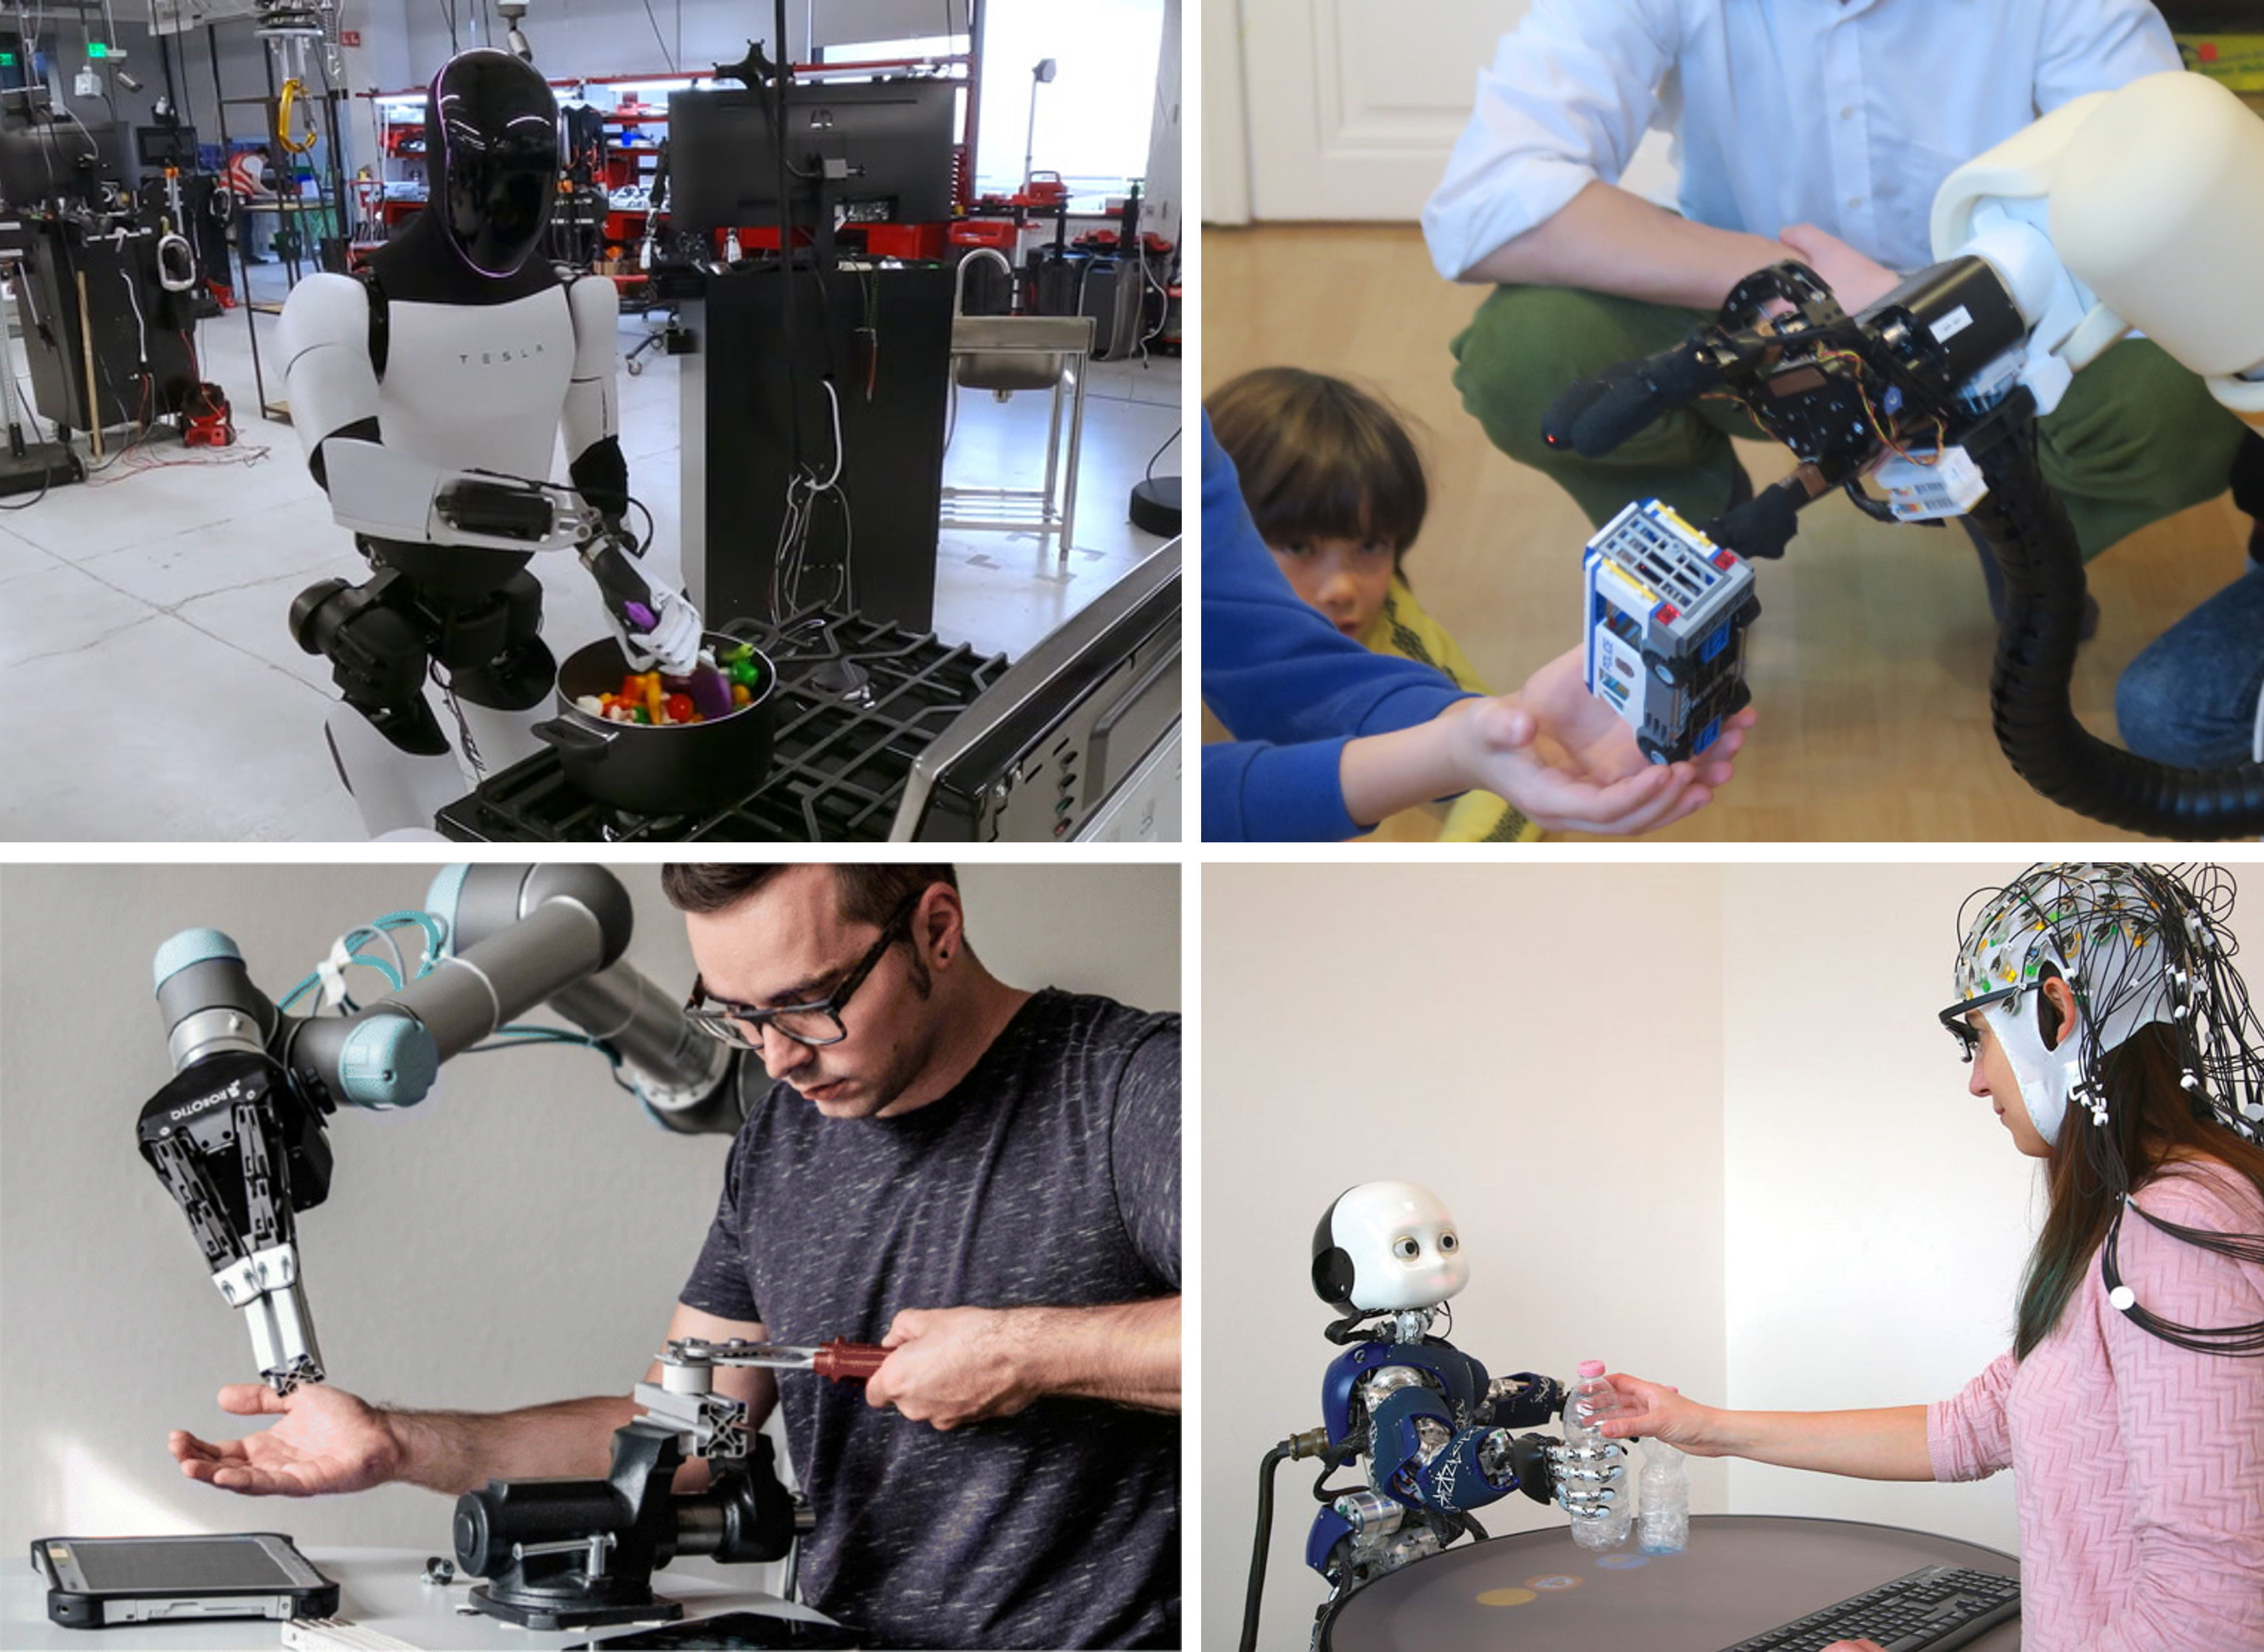
\includegraphics[width=0.8\textwidth]{general1}}
 	\caption{ورود ربات ها به دنیای تعامل با انسان ها
 		%\cite{kim2016integrated}
 	}
 	\label{fig:general1}
 \end{figure}


\section{نحوه‌ی ادراک  ربات ها از محیط و اشیاء}
ربات‌ها به طور معمول از حسگرهای گوناگونی برای درک محیط استفاده می‌کنند. این حسگرها را می‌توان به دو دسته  کلی غیرتماسی و تماسی تقسیم کرد. انواع دوربین های دوبعدی، تشخیص عمق و رادار لیزری
\LTRfootnote{LIDAR}
نمونه‌ای از حسگرهای غیرتماسی هستند که اطلاعاتی در مورد اشیاء و محیط، بدون تماس فیزیکی، فراهم می‌کنند. این حسگرها به در خدمت روش های یادگیری ماشین، توانسته‌اند ربات‌ها را قادر سازند تا برنامه‌ریزی صحیحی برای تعامل با محیط انجام دهند و محل مناسب برای گرفتن اشیاء را تشخیص دهند.
\cite{tian2023data,hosseini2024multi,beigy2024explorable,sabzejou20232d,moghadam2023grasp}
\subsection{آیا بینایی به تنهایی کافیست؟}

با وجود پیشرفت‌های چشمگیر در حوزه‌ی بینایی ماشین
\LTRfootnote{Computer Vision}
و کنترل ربات بر مبنای این حس
\LTRfootnote{Vision-based Robot Control}
،بینایی به تنهایی برای انجام وظایف پیچیده کافی نبوده و قادر به درک ویژگی‌های فیزیکی اشیا مانند نرمی، شکنندگی، بافت سطح یا نیروی اعمالی نیست. حس بینایی نمی‌تواند به طور مستقیم و در لحظه اصطکاک و یا لغزش بین چنگک و جسم را تشخیص دهد؛ با تکیه بر بینایی نمی‌توان میزان نیروی اعمال شده به یک جسم نرم یا شکننده را کنترل کرد.
\cite{yamaguchi2019recent,chi2018recent}
همچنین، هنگامی که چنگک
\LTRfootnote{Gripper}
 یک جسم را می‌گیرد، آن جسم ممکن است دید حسگر بینایی را مسدود کند و اطلاعات لحظه‌ای مربوط به تماس از دست برود. این ناتوانی‌ها چالشی بزرگ برای تعامل پایدار و مفید با اشیاء ایجاد می‌کنند. در نتیجه واضح است که صرفاً اتکا به حس بینایی برای انجام وظایف پیچیده و ظریف کافی نیست و نیاز به اطلاعات حسی دیگری به‌ خصوص حس لامسه ضروری است.
\subsection{لزوم حس لامسه در ربات}
حس لامسه یکی از مؤلفه‌های اصلی برای درک محیط توسط ربات، به‌ویژه در تعامل فیزیکی با اشیا، است. این حس امکان اندازه‌گیری نیروهای عمودی و جانبی، تشخیص برخورد با سایر عوامل موجود در محیط واعمال نیروی مناسب در حین انجام وظایف را فراهم می‌کند.
\cite{zou2017novel, yousef2011tactile}
وجود حس لامسه برای انجام وظایفی که نیازمند کنترل دقیق نیرو و تعامل ایمن با اشیای ظریف هستند، ضروری است. به عنوان مثال، در وظایف مونتاژ، جابه‌جایی مواد غذایی، یا تعامل با انسان، حس لامسه نقشی کلیدی در جلوگیری از آسیب به اشیا و بهبود عملکرد کلی ایفا می‌کند.
همچنین، پژوهش‌ها نشان داده‌اند که ادغام داده‌های لامسه و بینایی می‌تواند ادراک ربات را مشابه عملکرد انسان بهبود و سازگاری ربات با شرایط ناشناخته را افزایش دهد.
\cite{dahiya2013robotic}

\subsection{اهمیت حس لامسه در چنگک های رباتی}
عملگرهای نهایی 
\LTRfootnote{End-Effectors}
و به‌ویژه چنگک‌ها، اصلی‌ترین رابط مکانیکی بین ربات و محیط پیرامون آن محسوب می‌شوند. آن‌ها نقطه اصلی تماس ربات با اشیاء هستند و بخش عمده‌ای از وظایف یک ربات، از جمله گرفتن، جابجایی و دستکاری اشیاء، توسط این ابزارها انجام می‌شود. در دهه‌های گذشته، تمرکز اصلی در رباتیک صنعتی بر روی وظایف تکراری و از پیش تعریف‌‌شده در محیط‌های کاملاً کنترل‌شده بود؛ اما امروزه با گسترش کاربرد ربات‌ها در حوزه‌هایی مانند خدمات، پزشکی، کشاورزی و تعامل مستقیم با انسان، نیاز به ساختاری امن، قابل اعتماد و هوشمند برای این تعاملات به یکی از اهداف اصلی حوزه رباتیک تبدیل شده است.
\cite{broadbent2017interactions}
عملکرد قابل اطمینان برای چنگک‌های رباتی بسیار فراتر از یک گرفتن و رها کردن ساده است. یک گرفتن موفق نه تنها مستلزم لمس جسم هدف می‌باشد، بلکه باید از خطراتی مانند لغزش
\LTRfootnote{Slippage}
  شئ هدف و یا آسیب رساندن به آن به دلیل اعمال نیروی بیش از حد نیز جلوگیری شود. اینجاست که محدودیت‌های سیستم‌های کنترلی که صرفاً بر حس بینایی متکی هستند، آشکار می‌شود. اگرچه بینایی در مراحل اولیه مانند شناسایی و مکان‌یابی شیء نقشی حیاتی دارد، اما در لحظه تماس فیزیکی، به دلیل انسداد دید توسط خود چنگک و عدم توانایی درک خواص فیزیکی نامشهود، کارایی خود را از دست می‌دهد.
 \cite{malis2002survey}
 \\
 وجود حس لامسه در چنگک‌ها، این شکاف اطلاعاتی را پر کرده و کلید دستیابی به دستکاری 
 \LTRfootnote{Manipulation}
 پایدار، دقیق و هوشمند است. حسگرهای لامسه با فراهم آوردن اطلاعات بی‌درنگ از شرایط تماس، قابلیت‌های چنگک را به شکل چشمگیری افزایش می‌دهند. چند نوع از اطلاعاتی که حسگرهای لامسه می‌توانند فراهم کنند، شامل موارد زیر می‌شود:
 \begin{itemize}
 	\item \textbf{اندازه‌گیری نیرو و گشتاور } 
 	\\
حسگرهای لامسه می‌توانند مقادیر دقیق نیروهای نرمال و برشی اعمال‌شده بر سطح شیء را اندازه‌گیری کنند. این اطلاعات به سیستم کنترل اجازه می‌دهد تا نیروی گرفتن را به طور پیوسته تنظیم کند؛ نیروی اعمالی نباید آن‌قدر زیاد باشد که به جسم آسیب بزند و در عین حال، نباید آن‌قدر کم باشد که جسم بلغزد و از دست ربات رها شود
 	\cite{piga2023adaptive}
 	. توانایی انسان در بلند کردن یک تخم‌مرغ بدون شکستن آن، مثال بارزی از همین تنظیم دقیق نیرو بر اساس بازخورد لمسی است.
 	 
 	 \item \textbf{تشخیص لغزش} 
 	 \\
لغزش یکی از پدیده‌های دینامیکی کلیدی در حین دستکاری اشیاء است. حسگرهای لامسه، به‌ویژه آن‌هایی که به ارتعاشات فرکانس بالا حساس هستند، می‌توانند شروع لغزش را در مراحل اولیه تشخیص دهند. این تشخیص زودهنگام به کنترل‌کننده ربات فرصت می‌دهد تا به سرعت نیروی گرفتن را افزایش داده و از افتادن شیء جلوگیری کند.
 	 \cite{kyberd2023slip,costanzo2018slipping}
 	 
 	 \item \textbf{شناسایی موقعیت و توزیع تماس}
آرایه‌ای از حسگرهای لامسه می‌تواند نقشه‌ای از توزیع فشار بر روی سطح انگشتان چنگک ربات ایجاد کند. این اطلاعات برای تعیین مرکز فشار، تشخیص جهت‌گیری شیء در دست و اطمینان از یک گرفتن پایدار بسیار ارزشمند است.
\cite{khamis_novel_2019,de2022soft,wang_low-cost_2016}
\\
 \begin{figure}[ht]
	\centerline{\includegraphics[width=0.8\textwidth]{general2}}
	\caption{نمونه‌ای از تعامل چنگک های رباتی با اشیاء ظریف و نرم
		\cite{zhang2020state}
	}
	\label{fig:general1}
\end{figure}
 \end{itemize} 
\subsection{الهام از زیست: حس لامسه در انسان}
طبیعت در طول میلیون‌ها سال فرگشت، سیستم‌های بهینه‌ای را برای تعامل با محیط فیزیکی توسعه داده است. در میان این سیستم‌ها، حس لامسه انسان به عنوان پیچیده‌ترین، کارآمدترین و چندوجهی‌ترین سیستم حسی برای تعامل یا اشیاء شناخته می‌شود. پوست انسان، به‌ویژه در ناحیه نوک انگشتان، یک شاهکار مهندسی بیولوژیک است که ترکیبی از حساسیت بالا، استحکام، قابلیت ترمیم و توانایی پردازش اطلاعات پیچیده را به نمایش می‌گذارد. به همین دلیل، درک عمیق سازوکار حس لامسه انسان، نه تنها الهام‌بخش، بلکه یک نقشه راه ضروری برای طراحی و ساخت  حسگرهای رباتیکی است. 
\cite{silvera2015artificial}
موفقیت سیستم لامسه انسان در دستیابی به تعامل ماهرانه
\LTRfootnote{Dexterous Manipulation} 
 بر دو اصل بنیادین استوار است که در این پژوهش نیز به عنوان انگیزه اصلی مورد توجه قرار گرفته‌اند: 
 \textbf{اهمیت چندوجهی بودن ادراک حسی و ویژگی نرم و ارتجاعی نوک انگشتان.}
 در ادامه این بخش، این دو اصل کلیدی با جزئیات بیشتری بررسی می‌شوند.
\subsubsection{ ماهیت چندوجهی حس لامسه انسان}

پوست انسان یک حسگر یکپارچه و همگن نیست، بلکه مجموعه‌ای از گیرنده‌های حسی تخصصی است که هرکدام به نوع خاصی از محرک‌های لمسی با پهنای باند متفاوت پاسخ می‌دهند. این گیرنده‌های مکانیکی
 \LTRfootnote{Mechanoreceptors}
 که مسئول تبدیل محرک‌های لمسی به سیگنال‌های عصبی هستند، عمدتاً در لایه‌های روپوست
 \LTRfootnote{Epidermis}
و لایه‌ی میانی
\LTRfootnote{Dremis}
قرار دارند. در پوست بدون مو  مانند نوک انگشتان، که برای تعامل با اشیاء تکامل یافته‌اند، چهار نوع اصلی گیرنده مکانیکی وجود دارد که هر یک وظیفه مشخصی بر عهده دارند.
 \cite{wettels2011biomimetic, chi2018recent}.
\\
\begin{figure}[t]
	\centering
	\centerline{\includegraphics[width=0.8\textwidth]{Human_skin}}
	\caption{مقطعی از ساختار پوست انسان و محل قرارگیری چهار گیرنده لامسه اصلی در نوک انگشتان
		\cite{silvera2015artificial}
		. }
	\label{fig:skin_cross_section}
\end{figure}
این چهار گیرنده بر اساس سرعت پاسخشان به محرک‌های لامسه، به دو دسته اصلی تقسیم می‌شوند. دسته اول، گرینده های فرکانس پایین هستند که تا زمانی که محرک فیزیکی وجود داشته باشد، به طور پیوسته سیگنال عصبی تولید می‌کنند و مسئول درک اطلاعات استاتیک مانند نیرو هستند. دسته دوم، گیرنده های فرکانس بالا می‌باشند که فقط به تغییرات در محرک فیزیکی، یعنی در لحظه شروع و پایان تماس، پاسخ می‌دهند؛ این گروه مسئول درک اطلاعات دینامیک و گذرا هستند. این تقسیم‌بندی، اساس توانایی انسان در درک همزمان نیروهای مانا و پدیده‌های دینامیکی مانند لغزش است.
\begin{table}[ht]
	\caption{خلاصه‌ای از ویژگی‌ها و وظایف گیرنده‌های لامسه در نوک انگشتان انسان
\cite{chi2018recent}	
.}
	\label{tab:mechanoreceptors}
	\centering
	\onehalfspacing
	\begin{tabular}{|r|r|r|r|}
		\hline
		\textbf{نام گیرنده} & \textbf{محدوده فرکانس (هرتز)} &  \textbf{وظیفه اصلی} & \textbf{معادل در رباتیک} \\
		\hline \hline
		دیسک‌های مرکل
		\footnotemark
		
		 &  ۰.۳ - ۳ & فشار استاتیک&  نیروی گرفتن \\
		پایانه‌های رافینی
		\footnotemark
		 &  تا ۱۵ & کشش پوست، & نیروی مماسی\\
		گویچه‌های مایسنر
		\footnotemark
		 & ۳ - ۴۰ & تماس اولیه، لغزش آرام & تشخیص رویداد تماس \\
		گویچه‌های پاچینی 
		\footnotemark
		& ۱۰ - ۵۰۰ & ارتعاشات، لغزش  & تشخیص لغزش \\
		\hline
	\end{tabular}
\end{table}
\LTRfootnotetext[13]{Merkel's disks}
\LTRfootnotetext[14]{Ruffini's corpuscles}
\LTRfootnotetext[15]{Meissner corpuscles}
\LTRfootnotetext[16]{Pacinian corpuscles}
\\
این «تفکیک وجه ها» به مغز اجازه می‌دهد تا اطلاعات غنی و متنوعی را به صورت موازی پردازش کند و این همان اصلی است که این پژوهش با طراحی و ساخت یک حسگر چندوجهی
\LTRfootnote{Multi-modal}
قصد پایبندی به آن را دارد.
این تقسیم‌بندی پیچیده نشان می‌دهد که چرا تلاش برای ساخت یک حسگر لامسه رباتیک با تنها یک نوع تبدیل (مثلاً فقط اندازه‌گیری فشار) برای دستیابی به مهارت انسان کافی نیست. یک حسگر لامسه زیست الهام
\LTRfootnote{Biomimetic}
 واقعی باید بتواند اطلاعات استاتیک و دینامیک را در پهنای باندهای مختلف به صورت همزمان دریافت و پردازش کند
 \cite{silvera2015artificial}.
  این دقیقاً همان هدفی است که در این پژوهش با ترکیب یک حسگر فشار بارومتریک (برای درک اطلاعات استاتیک مشابه مرکل)، حسگرهای اثر هال (برای درک کشش و نیروی برشی مشابه رافینی)، حسگر دما و یک میکروفون (برای درک ارتعاشات فرکانس بالا مشابه پاچینی) دنبال شده است.


\subsubsection{ویژگی نرم و ارتجاعی نوک انگشتان}

دومین اصل کلیدی در موفقیت حس لامسه انسان، ماهیت فیزیکی خود انگشتان است. نوک انگشتان انسان از بافت نرم و ارتجاعی ساخته شده است که این ویژگی مزایای مکانیکی مهمی را در حین تعامل با اشیاء فراهم می‌کند.
یکی از مهم‌ترین این مزایا، \textbf{افزایش سطح تماس و پایداری گرفتن} است. هنگامی که یک انگشت نرم با یک جسم تماس پیدا می‌کند، تغییر شکل داده و خود را با شکل سطح جسم تطبیق می‌دهد. این امر باعث افزایش قابل توجه سطح تماس در مقایسه با یک انگشت صلب می‌شود. سطح تماس بزرگتر، نیروی گرفتن را بر روی ناحیه وسیع‌تری توزیع می‌کند که این امر اولاً خطر آسیب به اشیاء شکننده را کاهش می‌دهد و ثانیاً با افزایش مقاومت در برابر گشتاورهای خارجی، یک گرفتن بسیار پایدارتر ایجاد می‌کند
 \cite{yousef2011tactile}.

علاوه بر این، نرمی انگشتان بسیاری از عدم قطعیت‌ها و خطاهای کوچک در مکان‌یابی و جهت‌گیری شیء را جبران می‌کند. نیازی نیست که ربات موقعیت دقیق جسم را بداند؛ بافت نرم انگشت، خود را با ناهمواری‌ها و شکل‌های نامنظم تطبیق می‌دهد و یک تماس کامل را تضمین می‌کند. این ویژگی، نیاز به الگوریتم‌های کنترلی پیچیده را کاهش داده و به گرفتن قابل اطمینان کمک می‌کند.

نهایتاً، این تغییرشکل‌پذیری منجر به تقویت سیگنال‌های لمسی می‌شود. تغییر شکل پوست در اطراف یک شیء، الگوهای فشار و کشش منحصربه‌فردی را بر روی گیرنده‌های مکانیکی زیرین ایجاد می‌کند. به عنوان مثال، لبه‌های یک جسم باعث ایجاد تمرکز تنش در پوست می‌شوند که این امر به گیرنده‌های مرکل کمک می‌کند تا شکل را با دقت بیشتری تشخیص دهند. این پدیده به ربات نیز کمک می‌کند تا اطلاعات غنی‌تری از تماس استخراج کند.
\cite{silvera2015artificial}
این مزایا نشان می‌دهد که طراحی یک حسگر لامسه موفق، تنها به انتخاب مبدل‌های الکترونیکی مناسب محدود نمی‌شود، بلکه به طراحی مکانیکی و مواد به کار رفته در ساختار آن نیز بستگی دارد. استفاده از مواد نرم مانند سیلیکون در ساخت حسگرهای رباتیک، تلاشی برای تقلید از این ویژگی‌های سودمند فیزیکی انگشتان انسان است.

در نتیجه، با الهام از این دو اصل، این  پژوهش نه تنها بر توسعه یک سیستم الکترونیکی چندوجهی تمرکز داشته، بلکه این سیستم را در یک ساختار نرم و ارتجاعی ادغام می‌کند تا به ترکیبی بهینه از درک حسی و سازگاری مکانیکی، مشابه دست انسان، دست یابد.

\section{انواع روش های تبدیل در ساخت حسگر لامسه و مروری بر کار‌های پیشین}
\subsection{روش های مبتنی بر پیزوالکتریک}

از منظر لغوی، پیزو به معنی فشار است و ترکیب پیزو الکتریک
\LTRfootnote{Piezo-electric}
 به موادی اطلاق می‌شود که در اثر اعمال فشار، سیگنال الکتریکی از خود تولید می‌کنند. این حسگر‌ها از پدیده‌ای فیزیکی به نام اثر پیزوالکتریک بهره می‌برند. این اصطلاح علمی به معنای «الکتریسیته ناشی از فشار» است و به توانایی برخی مواد خاص برای تولید یک ولتاژ یا بار الکتریکی در پاسخ به کرنش مکانیکی یا فشار اشاره دارد. ساختار بلوری این مواد به گونه‌ای است که در حالت عادی، بارهای مثبت و منفی به طور متقارن توزیع شده و اثر یکدیگر را خنثی می‌کنند، اما با اعمال فشار یا نیروی مکانیکی، این تقارن به هم می‌خورد و بارهای الکتریکی مثبت و منفی در دو طرف ماده ظاهر می‌شوند، که منجر به تولید یک ولتاژ قابل اندازه‌گیری می‌گردد. این پدیده در موادی مانند کریستال‌های کوارتز 
\LTRfootnote{Quartz crystals}،
 سرامیک‌های پیزوالکتریک مانند PZT
 \LTRfootnote{Lead Zirconate Titanate}
  و برخی پلیمرها مانند PVDF
 \LTRfootnote{Polyvinylidene Fluoride}) مشاهده می‌شود.
\\
برای کاربردهای حسگر لامسه، مواد پیزوالکتریک به دلیل ویژگی‌های منحصربه‌فردشان بسیار مناسب هستند. این حسگرها نیازی به منبع تغذیه خارجی ندارند و می‌توانند به صورت فعال
\LTRfootnote{Active}
 عمل کنند که این ویژگی، مصرف انرژی را به شدت کاهش می‌دهد. مهم‌ترین مزیت این مکانیزم، پاسخ دینامیکی فوق‌العاده سریع و حساسیت بسیار بالا به تغییرات نیرو است. این خصوصیت آن‌ها را برای تشخیص ارتعاشات با فرکانس بالا و لغزش‌های بسیار جزئی
 \LTRfootnote{Micro-Slip}
 ایده‌آل می‌کند. در واقع، یک حسگر پیزوالکتریک می‌تواند لغزش یک جسم را در کسری از ثانیه تشخیص دهد که این امر به ربات اجازه می‌دهد قبل از افتادن کامل شیء، نیروی عمودی را اصلاح کند. پژوهش های متعددی در این زمینه انجام شده‌است که به ساخت حسگرهای لامسه پیزوالکتریک برای کاربردهای مختلف پرداخته‌اند. برای مثال، در پژوهش 
\cite{nasserii2011Piezo}
  نویسندگان به طراحی و ساخت یک حسگر بر اساس تغییر امپدانس کریستال پیزوالکتریک برای اندازه‌گیری نیروی اعمالی می‌پردازد. این حسگر با سنجش ولتاژ خروجی ناشی از فشار، توانایی تخمین نیروی اعمال شده را دارد. نتایج این پژوهش نشان داد که با توجه به طراحی ساده، حسگر ساخته شده قابلیت تغییر اندازه و شکل را دارد و برای کاربردهایی مانند جراحی‌های کم‌تهاجمی مناسب است. با این حال، جزئیات دقیق و کمی از دقت و حساسیت آن ارائه نشده است.
  همچنین،
  \cite{spanu2016PVDF}
   یک حسگر لمسی بسیار حساس را معرفی می‌کنند که از یک پلیمر پیزوالکتریک (PVDF) به همراه ترانزیستور ارگانیک استفاده می‌کند و برای پوست رباتیک مطرح شده است. حسگر مذکور توانایی اندازه‌گیری نیروهایی که به کوچکی 20mN را دارد.
   در مقاله‌ی 
   \cite{qi2023PVDF}
نویسندگان به بررسی انواع مواد قابل استفاده برای طراحی حسگر لامسه مبتنی بر پیزوالکتریک می‌پردازند.
    پژوهش‌هایی مانند
 \cite{wang2019PiezoArray,huang2024piezo,yu2016PiezoArray}
   به ساخت آرایه‌های حسگر پیزوالکتریک انعطاف‌پذیر برای اندازه‌گیری نیروهای سه‌محوری و تشخیص لغزش در حین گرفتن اشیاء پرداخته اند. سرعت خوانش اطلاعات در این پژوهش‌ها 5 تا 400 هرتز و در 
   \cite{huang2024piezo}
   1900 هرتز می‌باشد. بازه‌ی اندازه‌گیری نیرو به ترتیب 15، 11 و \LR{1.5} نیوتن برای محور عمودی گزارش شده است.
   
\begin{figure}[t]
	\centering
	\includegraphics[width=0.8\textwidth]{wang_piezo}
	\caption{شمای کلی حسگر ارائه شده در پژوهش 
		\cite{wang2019PiezoArray}
		. }
	\label{fig:wang_piezo}
\end{figure}
   
\begin{table}[ht]
	\centering
	\caption{مقایسه سنسورهای لمسی پیزوالکتریک گزارش‌شده در مقالات مختلف}
	\label{tab:piezo_sensors}
	\onehalfspacing
	\begin{tabular}{|r|r|r|r|r|r|}
		\hline
		\textbf{مرجع} & \textbf{سال} & \textbf{تعداد المان‌های حسی}  & \textbf{بازه نیرو} & \textbf{حساسیت} & \textbf{ماده پیزوالکتریک} \\ \hline \hline
		
		\cite{nasserii2011Piezo} & 2011 & 1 &$12 \: N$ & $33.47 \frac{mV}{N}$ & سرامیک پیزو \\ \hline
		
		\cite{spanu2016PVDF} & 2016 & 1 & 
		 $3.5 \: N$ & $3 \frac{nA}{N}$ & PVDF + Organic transistor \\ \hline
		
		\cite{yu2016PiezoArray} & 2016 & $2 \times 3 $ & $1.5 \: N$ & 
		$6.62 \frac{pC}{N}$ & \LR{PVDF} \\ \hline
		
		\cite{wang2019PiezoArray} & 2019 & $3 \times 3 $& $15 \: N$ &  $210 \frac{mV}{N}$ & PVDF \\ \hline
		
		\cite{huang2024piezo} & 2024 &$ 3‌ \times 3 $& $11 \: N$ & $35.6 \frac{mV}{N}$ & PVDF-based (rigid-in-soft) \\ \hline
		
	\end{tabular}
\end{table}

\subsection{روش های مبتنی بر پیزو مقاومت}
مکانیزم پیزومقاومتی یکی از بنیادی‌ترین و پرکاربردترین اصول در طراحی حسگرهای لامسه است که در سال‌های اخیر با توسعه مواد پیشرفته و ساختارهای میکرو و نانومتری توجه بسیاری را به خود جلب کرده است. اساس این روش بر این واقعیت استوار است که مقاومت الکتریکی یک ماده رسانا یا نیمه‌رسانا تحت تأثیر تغییرات مکانیکی نظیر فشار، کشش یا خمش تغییر می‌کند. این تغییر مقاومت را می‌توان به‌صورت یک سیگنال الکتریکی خواند و متناسب با آن شدت یا نوع تحریک مکانیکی را تعیین نمود. در واقع، تحریک مکانیکی به‌طور غیرمستقیم به یک پاسخ الکتریکی تبدیل می‌شود و همین امر امکان استفاده از آن را در ساخت پوست‌های مصنوعی، پروتزهای هوشمند و ربات‌های دارای قابلیت حس لامسه فراهم می‌سازد.

از دیدگاه فیزیکی، تغییرات مقاومت الکتریکی در یک ماده‌ی پیزو دو منشاء می‌تواند داشته باشد؛ منشاء اول تغییرات هندسی ماده مذکور است. همان‌طور که در رابطه‌ی کلاسیک مقاومت 
\begin{equation}\label{eq:piezoRes1}
	R=\rho\frac{l}{A}
\end{equation}
​

دیده می‌شود، اعمال تنش باعث افزایش طول و کاهش سطح مقطع یک رسانا می‌گردد و در نتیجه مقاومت آن تغییر می‌کند. دلیل دوم به تغییر مقاومت ویژه یا همان مقاومت ذاتی ماده مربوط است. در نیمه‌رساناهایی مانند سیلیکون و ژرمانیم، تنش مکانیکی موجب تغییر ساختار باند انرژی می‌شود و این تغییر، تحرک بارهای الکتریکی و چگالی آنها را دگرگون کرده و در نهایت مقاومت ویژه را تغییر می‌دهد
\begin{figure}[ht]
	\centering
	\includegraphics[width=0.8\textwidth]{piezoRes_ahmed2013mems}
	\caption{المان پیزومقاومتی استفاده شده در
		\cite{ahmed2013piezores}
		از جنس
		\LR{Si3N4 }}
		\label{fig:ahmed_piezores}
	\end{figure}
	. علاوه بر این دو منشاء، در ترکیباتی که شامل نانومواد کربنی، نانوسیم‌های فلزی یا ذرات رسانا هستند، تغییر مقاومت بیشتر ناشی از تغییر در مقاومت تماسی میان ذرات و پدیده‌هایی مانند تونل‌زنی کوانتومی
	\LTRfootnote{Quantum Tunneling Effect}
	است. زمانی که فشار به چنین ساختارهایی اعمال می‌شود، فاصله میان ذرات کاهش یافته و تماس‌های الکتریکی جدیدی ایجاد می‌شود که این فرایندها تغییرات شدیدی در مقاومت الکتریکی ایجاد می‌کنند.
	\cite{xi2024mechanisms}

	
	\begin{figure}[ht]
		\centering 
		\subfloat[مقوامت الکتریکی نسبت به نیرو\cite{drimus2014piezores}]{ \label{fig:pizeoResplots:RF}
			\includegraphics[width=0.5\textwidth]{drimus_2014_RF}}
		%\hspace{2mm}
		\subfloat[پسماند الکتریکی هنگام اعمال و برداشتن نیرو\cite{koiva2013piezores}]{ \label{fig:pizeoResplots:hysteresis}
			\includegraphics[width=0.5\textwidth]{koiva2013_piezoHysteresis}}%
		\caption{نمودارهای مشخصه برای حسگر های پیزومقاومتی.
		\ref{fig:pizeoResplots:RF}: مقاومت الکتریکی بر حسب نیرو.
	\ref{fig:pizeoResplots:hysteresis}پسماند سیگنال
\cite{koiva2013piezores}}
		\label{fig:pizeoResplots} %% label for entire figure
	\end{figure}
	
	
	
	پژوهش‌های متعددی برای بهبود حساسیت و محدوده‌ی عملکرد حسگرهای پیزومقاومتی انجام شده است. به عنوان نمونه، پژوهشگران در
	\cite{jing2022ag} 
	یک حسگر پیزومقاومتی انعطاف‌‌پذیر مبتنی بر نانوسیم‌های نقره و 
	\LR{PVDF}
	توسعه دادند که دارای ساختار سه‌بعدی متخلخل بود و به دلیل توزیع یکنواخت نانوسیم‌ها، حساسیت مناسبی در بازه ۰ تا ۱۰۰ کیلوپاسکال به دست آورد.  
	
	نمونه‌ی دیگر، پژوهش \cite{zhao2022pdms} است که از ترکیب نانولوله‌های کربنی و گرافن روی بستر
	\LR{PDMS}\LTRfootnote{Poly dimethyl siloxane}
	متخلخل استفاده کردند. آنها با ایجاد میکروحفره‌های یکنواخت در بستر از طریق گرمایش مایکروویوی، سطح تماس بسیار زیادی برای نانومواد رسانا فراهم آوردند. نتیجه این طراحی، دستیابی به حساسیتی در حدود \(300.31 \, kPa^{-1}\) در فشارهای پایین (۰ تا ۵۰ کیلوپاسکال) بود.  
	
	مکانیزم پیزومفاومتی محدودیت هایی نیز دارد؛ به طور مثال در شکل
	\ref{fig:pizeoResplots:RF}
	مشاهده می‌شود که رفتار غیرخطی حسگر در بازه‌های وسیع فشار باعث می‌شود رابطه بین نیروی واردشده و تغییر مقاومت همیشه خطی نبوده و کالیبراسیون دقیق را دشوار می‌سازد.
	علاوه بر این، با توجه به شکل 
	\ref{fig:pizeoResplots:hysteresis}
	وجود پسماند
	\LTRfootnote{Hysteresis}
	در پاسخ حسگر باعث می‌شود که مقادیر خروجی در هنگام اعمال و برداشت نیرو یکسان نباشد و دقت اندازه‌گیری کاهش یابد. عامل دیگر، حساسیت بالا به تغییرات دما است، زیرا افزایش دما می‌تواند تحرک حامل‌های بار و نیز مقاومت ویژه ماده را تغییر دهد و در نتیجه پاسخ حسگر را تحت تأثیر قرار دهد. همچنین این دسته از حسگرها اغلب دارای زمان بازیابی طولانی پس از اعمال نیرو هستند، به این معنا که بازگشت به حالت اولیه در بسیاری از طراحی‌ها به کندی صورت می‌گیرد. این ویژگی‌ها موجب محدودیت در استفاده از حسگرهای پیزومقاومتی در محیط‌هایی با تغییرات سریع نیرو یا دما شده و پژوهشگران را به سمت توسعه راهکارهای جبرانی، طراحی ترکیبی با مکانیزم‌های دیگر و استفاده از مواد نوین سوق داده است.
	
	
	\begin{table}[ht]
		\centering
		\caption{مقایسه سنسورهای لمسی پیزومقاومتی گزارش‌شده در مقالات مختلف}
		\label{tab:piezo_res}
		\onehalfspacing
		\begin{tabular}{|r|r|r|r|r|r|}
			\hline
			\textbf{مرجع} & \textbf{سال} & \textbf{تعداد المان‌های حسی}  & \textbf{بازه نیرو} & \textbf{حساسیت} & \textbf{ماده پیزوالکتریک} \\ \hline \hline
			
			\cite{noda2006cantilever} & 2006 & 1 &$-5 \: kPa - 5\: kPa (shear)$ & $0.03\%$ & Silicone \\ \hline
			
			\cite{koiva2013piezores} & 2013 & 12 & 
			$10 \: N$ & $0.015\%$ & LCPT\footnotemark \\ \hline
			
			\cite{ahmed2013piezores} & 2013 & $6 \times 8 $ & $30 \: kPa$ & 
			$1.25 \frac{V}{N}$ & \LR{Nichrome} \\ \hline
			
			\cite{drimus2014piezores} & 2014 & $8 \times 8 $ & $10 \: kPa$ & 
			$--$ & \LR{Conductive rubber} \\ \hline
			
			\cite{jing2022ag} & 2022 &$1$& $100 \: kPa$ &  $0.009 kPa^{-1} $ & AgNws + PVDF \\ \hline
			
			\cite{hou2022fiber} & 2022 &$ 1 $& $150 \: kPa$ & $2.06 kPa^{-1} $ & Cu + PDMS (rigid-in-soft) \\ \hline
			
			\cite{zhao2022pdms} & 2022 &$ 1$& $200 \: kPa$ & $300.31 kPa^{-1} $ & PDMS \\ \hline
		\end{tabular}
	\end{table}
	\LTRfootnote[30]{Liquid Crystal Polymer Thermoplastic}
	
\subsection{روش های خازنی}

فناوری خازنی یکی از پرکاربردترین و منعطف‌ترین رویکردها در طراحی حسگرهای لامسه رباتیک است. این حسگرها به دلیل حساسیت بالا، مصرف توان پایین و قابلیت مجتمع‌سازی در مقیاس بزرگ، توجه بسیاری از محققان را به خود جلب کرده‌اند. فلسفه اصلی در این حسگرها، اندازه‌گیری تغییر ظرفیت یک خازن بر اثر تغییر مکانیکی در ساختار و هندسه آن است. این حسگرها معمولاً از ساختاری شبیه به یک خازن صفحه‌موازی تشکیل شده‌اند که ظرفیت آن‌ها از طریق رابطه کلاسیک زیر محاسبه می‌شود:
\begin{equation}
	C=\frac{\varepsilon_0 \varepsilon_r A}{d}.
	\label{eq:basicC}
\end{equation}
در این رابطه، $C$ ظرفیت خازن، $\epsilon_0$ ثابت گذردهی خلأ، $\epsilon_r$ ثابت دی‌الکتریک نسبی ماده بین صفحات، $A$ سطح هم‌پوشانی صفحات و $d$ فاصله بین آن‌ها است. یک نیروی خارجی می‌تواند با تغییر پارامترهای هندسی \textbf{فاصله ($d$)} یا \textbf{سطح هم‌پوشانی ($A$)}، ظرفیت خازن را تغییر دهد و این تغییر، پس از اندازه‌گیری، به مقدار نیرو نگاشت می‌شود \cite{chi2018recent}.

اگرچه ساختار صفحه‌موازی اساس کار این حسگرهاست، اما طراحی‌های متنوعی برای اندازه‌گیری انواع مختلف نیرو (عمودی و برشی) و افزایش چشمگیر حساسیت توسعه یافته است.با این حال، متداول‌ترین مکانیزم، مبتنی بر \textbf{ساختار صفحه‌موازی برای نیروی عمودی} است. در این طراحی، یک لایه الاستومری نرم به عنوان ماده دی‌الکتریک بین دو الکترود رسانای انعطاف‌پذیر قرار می‌گیرد. هنگامی که یک نیروی عمودی به سطح حسگر وارد می‌شود، لایه الاستومری فشرده شده، فاصله $d$ بین صفحات کاهش می‌یابد و در نتیجه، ظرفیت خازن ($C$) به صورت غیرخطی افزایش پیدا می‌کند.

یک نوآوری کلیدی برای بهبود عملکرد این ساختار، استفاده از میکرو-ساختارها
\LTRfootnote{Micro-structures}
 در لایه دی‌الکتریک است. به جای استفاده از یک لایه صاف، الاستومر به شکل ساختارهای ریزی مانند هرم
\LTRfootnote{Pyramid}،
 گنبد 
 \LTRfootnote{Dome}
  یا ستون
  \LTRfootnote{Pillar}
   قالب‌گیری می‌شود \cite{mannsfeld2010highly}. این معماری هوشمندانه، نیرو را در نقاط کوچکی متمرکز کرده و باعث تغییر شکل بسیار بزرگتری در فاصله ($d$) به ازای یک فشار معین می‌شود. وجود فضاهای خالی در بین این میکرو-ساختارها باعث می‌شود حسگر در محدوده فشارهای پایین بسیار نرم و حساس عمل کند. در نتیجه، حساسیت حسگر فشار که به صورت زیر تعریف می‌شود:
  
  \begin{equation}
  	S = (\Delta C/C_0)/\Delta P
  	\label{eq:sensC}
  \end{equation}
     به شدت افزایش یافته و امکان تشخیص تماس‌های بسیار آرام را فراهم می‌آورد \cite{zou2017novel}.

علاوه بر روش ساخت، پیشرفت در علم مواد نیز تأثیر مستقیمی بر بهبود عملکرد، انعطاف‌پذیری و حساسیت حسگرهای خازنی داشته است. انتخاب لایه دی‌الکتریک نقشی حیاتی دارد؛ 
\LR{PDMS}
 به دلیل انعطاف ‌پذیری عالی، پایداری شیمیایی و زیست ‌سازگاری، یکی از محبوب‌ترین گزینه‌هاست. برای کاربردهایی که به نرمی بیشتری نیاز دارند، از الاستومرهایی مانند
 \LR{Ecoflex}
   نیز استفاده می‌شود. جهت افزایش بیشتر حساسیت، این پلیمرها گاهی با نانوذراتی با ثابت دی‌الکتریک بالا
 \LTRfootnote{High-k}
  مانند
  \LR{TiO₂} \LTRfootnote{Titanium dioxide}
    یا 
      \LR{BaTiO₃} \LTRfootnote{Barium titanate}
     ترکیب می‌شوند. این کار باعث افزایش ظرفیت اولیه خازن شده و تغییرات نسبی ظرفیت ($\Delta C/C_0$) را قابل توجه‌تر می‌سازد \cite{zou2017novel}.
     
برای آنکه کل حسگر انعطاف‌پذیر باشد، لایه‌های رسانا الکترودها نیز باید قابلیت تغییرشکل داشته باشند. به همین منظور، به جای لایه‌های فلزی صلب، از مواد رسانای انعطاف‌پذیر استفاده می‌شود. گزینه‌هایی مانند نانولوله‌های کربنی
\LTRfootnote{CNTs}، 
 گرافن
 \LTRfootnote{Graphene}، 
 پلیمرهای رسانا و حتی  فلز مایع مانند 
 \LR{EGaIn}\LTRfootnote{
 	Eutectic Gallium-Indium}
  به حسگر اجازه می‌ده دهند تا به راحتی خم شده و بر روی سطوح منحنی پیچیده‌ای مانند نوک انگشت  ربات نصب شوند \cite{chi2018recent}.


	\begin{figure}[t]
	\centering
	\includegraphics[width=0.8\textwidth]{capacitive1}
	\caption{ساختار حسگر لامسه خازنی معرفی شده در
		\cite{pagoli2022large}.}
	\label{fig:CapStructure}
\end{figure}

با وجود مزایای فراوان، طراحی و پیاده‌سازی حسگرهای خازنی با چالش‌های مهندسی خاصی روبروست. مهم‌ترین چالش‌ها، حساسیت به نویز و خازن پارازیتی است. این حسگرها به دلیل داشتن امپدانس خروجی بالا، به راحتی تحت تأثیر نویزهای الکترومغناطیسی
\LTRfootnote{EMI}
  محیط قرار می‌گیرند. علاوه بر این، خازن‌های ناخواسته (پارازیتی) که بین خطوط سیگنال و زمین شکل می‌گیرند، می‌توانند تغییرات کوچک ظرفیت اصلی حسگر را پوشانده و دقت اندازه‌گیری را کاهش دهند. برای مقابله با این مشکل از راهکارهایی مانند شیلدینگ فعال
   \LTRfootnote{Active Shielding}،
    که در آن یک الکترود محافظ هم‌پتانسیل با الکترود اصلی نویز را منحرف می‌کند، و طراحی‌های تفاضلی
    \LTRfootnote{Differential Sensing}،
  که با اندازه‌گیری تفاوت بین دو خازن نویز حالت مشترک را حذف می‌کند، استفاده می‌شود \cite{tiwana2012review}.

چالش دیگر، پدیده پسماند است که از ماهیت گرانروی کشسان 
\LTRfootnote{Viscoelasticity}
پلیمرهای دی‌الکتریک ناشی می‌شود. این پدیده باعث می‌شود منحنی پاسخ حسگر در هنگام افزایش نیرو با منحنی آن در هنگام کاهش نیرو یکسان نباشد و منجر به خطا در اندازه‌گیری شود. انتخاب مواد با پسماند ذاتی کمتر و اعمال چرخه‌های بارگذاری اولیه برای پایدارسازی رفتار ماده، از راهکارهای کاهش این اثر است.

نهایتاً، مدارهای اندازه‌گیری برای این حسگرها باید از پیچیدگی و دقت بالایی برخوردار باشند. از آنجایی که تغییرات ظرفیت اغلب در محدوده بسیار کوچک فمتوفاراد تا پیکوفاراد  است، مدارهای تخصصی برای تبدیل دقیق این تغییرات به سیگنال دیجیتال یا ولتاژ ضروری هستند. مبدل‌های ظرفیت به ولتاژ 
\LTRfootnote{C-V Converters}
 و مدارهای مبتنی بر نوسان‌ساز
\LTRfootnote{Oscillator-based circuits} 
از جمله معماری‌های رایج برای این منظور هستند.


\begin{table}[ht]
	\centering
	\caption{مقایسه سنسورهای لمسی خازنی گزارش ‌شده در مقالات مختلف}
	\label{tab:cap}
	\onehalfspacing
	\begin{tabular}{|r|r|r|r|r|r|}
		\hline
		\textbf{مرجع} & \textbf{سال} & \textbf{تعداد المان‌های حسی}  & \textbf{بازه نیرو} & \textbf{حساسیت} & \textbf{ماده دی‌الکتریک} \\ \hline \hline
		
		 \cite{castelli2002integrated} 
		& 2002 
		& $4 \times 4$ 
		& \LR{Tecnoflon FLOR 421} 
		& $81 \: N$
		& -- \\
		 \hline
		
		\cite{ulmen2010robust} 
		& 2010 
		& $4 \times 4$ 
		& \LR{Silicone} 
		&$100 \: N$ 
		& $20 mN $ \\
		 \hline
		
		\cite{chen2013friction} 
		& 2013 
		& $2 \times 2$ 
		& \LR{PDMS} 
		&$2 \: N$ 
		& $0.38 \frac{pF}{N}$ \\
		\hline
		
		\cite{wang2016three} 
		& 2017 
		& $3 \times 3$ 
		& \LR{PDMS} 
		&$10 \: N$ 
		& $0.369 \frac{V}{N}$ \\
		\hline
		
		\cite{pagoli2022large} & 2022 &$10 \times 10$& $2.5 \: N$ & $125 mN $ & PDMS \\ \hline
	\end{tabular}
\end{table}


\subsection{مکانیزم نوری}
حسگرهای لمسی نوری، از ویژگی‌های فیزیکی نور و یازتاب آن برای اندازه‌گیری نیرو یا تغییر شکل استفاده می‌کنند و یک رویکرد جذاب را در طراحی حسگرهای لمسی ارائه می‌دهند. این حسگرها با تبدیل تغییرات مکانیکی به تغییرات نوری، سیگنال قابل اندازه‌گیری ایجاد می‌کنند و به دلیل ماهیت خود، نسبت به تداخلات الکترومغناطیسی و نویزهای الکتریکی مقاوم هستند. در واقع، این حسگرها با استفاده از یک دوربین یا فتودیود، تغییر شکل یک سطح کشسان را در اثر تماس مشاهده می‌کنند. این روش امکان استخراج اطلاعات غنی از تماس، از جمله نیروی نرمال، نیروی مماسی، لغزش و حتی بافت سطح را فراهم می‌کند.
مکانیزم عملکرد این حسگرها عموماً بر پایه تغییر مسیر، شدت یا زاویه نور در پاسخ به یک نیروی خارجی استوار است. این حسگرها معمولاً از سه بخش اصلی تشکیل شده‌اند: یک منبع نور، یک بستر تغییر شکل‌پذیر و یک گیرنده نور. با اعمال نیرو به سطح حسگر، بستر تغییر شکل داده و نور را به گونه‌ای تغییر می‌دهد که با ثبت این تغییرات می‌توان میزان نیرو، جابه‌جایی یا حتی بافت جسم را اندازه‌گیری کرد. برای مثال، حسگر 
\LR{GelSight}
 که در 
\cite{yuan2017gelsight}
 معرفی شد و یکی از شناخته‌شده‌ترین نمونه‌های این مکانیزم است، از یک لایه کشسان و یک دوربین در زیر آن استفاده می‌کند تا تغییرات شکل سطح را در اثر تماس ثبت کند. پژوهش‌های مختلفی نیز با استفاده از تعداد محدودی حسگر حساس به نور اقدام به اندازه‌گیری نیرو کرده اند که در ادامه به آنها خواهیم پرداخت.به طور کلی، یکی از مهم‌ترین مزایای حسگرهای نوری، وضوح و دقت فضایی بسیار بالا است که به آن‌ها اجازه می‌دهد جزئیات بسیار دقیق تغییر شکل سطح را ثبت کنند. این ویژگی برای تشخیص بافت و شکل اشیا بسیار حیاتی است. علاوه بر این، این حسگرها به دلیل عدم نیاز به تماس الکتریکی با محیط، در برابر تداخلات الکترومغناطیسی و رطوبت مقاوم هستند. این مزیت، آن‌ها را برای کاربرد در محیط‌های صنعتی یا پزشکی که شرایط محیطی دشوار است، مناسب می‌سازد. از سوی دیگر، حسگرهای نوری معایبی نیز دارند. طراحی این حسگرها، به‌ویژه انواع مبتنی بر دوربین، می‌تواند پیچیده و حجیم باشد. همچنین، عملکرد آن‌ها به شدت به نور محیطی حساس است و ممکن است تحت تأثیر آن قرار گیرد، که نیاز به سیستم‌های محافظت در برابر نور را ایجاد می‌کند. در نهایت، ساخت این حسگرها، به خصوص نمونه‌های با رزولوشن بالا و سه‌محوری، ممکن است پرهزینه باشد. با این حال، با وجود این چالش‌ها، حسگرهای لمسی نوری به دلیل توانایی در ارائه اطلاعات غنی از تماس، به عنوان یک راه‌حل کلیدی در حوزه رباتیک و دستکاری اشیاء مطرح هستند.
\subsubsection{روش های مبتنی بر دوربین و ثبت تصویر کلی لامسه}

حسگرهای لمسی مبتنی بر دوربین، یک رویکرد نوین و قدرتمند در حوزه حسگرهای لمسی برای کاربردهای رباتیک ارائه می‌دهند. برخلاف حسگرهای سنتی که به اندازه‌گیری مستقیم نیرو می‌پردازند، این حسگرها از یک سیستم بینایی برای اندازه‌گیری هندسه و تغییر شکل سطح تماس استفاده می‌کنند. این روش به ربات امکان می‌دهد تا اطلاعات غنی و دقیقی از تماس را با وضوح فضایی بسیار بالا به دست آورد.
یکی از شناخته‌شده‌ترین و مهم‌ترین پژوهش‌ها در این دسته، توسعه حسگر لمسی نوری مبتنی بر بینایی با نام Gelsight است. مکانیزم عملکرد GelSight بر اساس اندازه‌گیری مستقیم تغییر شکل یک سطح الاستومری نرم است. این حسگر دارای یک سطح تماس شفاف و نرم است که با یک لایه از ذرات ریز براق (مانند پودر آلومینیوم) پوشانده شده است. یک منبع نور داخلی این سطح را روشن می‌کند و یک دوربین کوچک که در پشت حسگر قرار گرفته، تصویر آن را ثبت می‌کند.


زمانی که حسگر با یک جسم تماس پیدا می‌کند، سطح الاستومری تغییر شکل می‌دهد و خود را با هندسه دقیق جسم تطبیق می‌دهد. این تغییر شکل باعث تغییر در الگوی نور منعکس‌شده می‌شود. برآمدگی‌ها، ناهمواری‌ها و لبه‌های جسم باعث ایجاد سایه‌ها و تغییر در شدت نور می‌شوند. از طریق تحلیل تصویر ثبت‌شده توسط دوربین، می‌توان با استفاده از الگوریتم‌های پردازش تصویر، اطلاعات هندسی سطح تماس و همچنین اطلاعات مربوط به کشش روی سطح را استنباط کرد.
\begin{figure}[t]
	\centering
	\includegraphics[width=0.8\textwidth]{gelsight1}
	\caption{ساختار حسگر لامسه 
		\LR{Gelsight} معرفی شده در
		\cite{yuan2017gelsight}.}
	\label{fig:gelsight1}
\end{figure}

برخلاف حسگرهای لمسی سنتی که صرفاً نیروی تماس را اندازه‌گیری می‌کنند، GelSight قادر به اندازه‌گیری هندسه تماس با وضوح فضایی بسیار بالا است. این حسگر به طور همزمان می‌تواند تغییر شکل عمودی (فشار) و جانبی (کشش) را اندازه‌گیری کند. از این اطلاعات می‌توان برای استنباط نیروی تماس، گشتاور و لغزش استفاده کرد. توانایی این حسگر در درک دقیق شکل و بافت جسم، آن را برای وظایف پیچیده دستکاری، مانند گرفتن اشیاء با اشکال نامنظم یا بافت‌های ظریف، بسیار مناسب می‌سازد. با وجود مزایای متعدد حسگرهای لمسی مبتنی بر دوربین مانند GelSight در زمینه دقت و رزولوشن بالا، این سیستم‌ها با چالش‌ها و محدودیت‌هایی نیز روبرو هستند که استفاده از آن‌ها را در برخی شرایط خاص دشوار می‌سازد.
یکی از اصلی‌ترین معایب، حساسیت به نور محیطی است. از آنجا که عملکرد این حسگر به تحلیل تصویر نوری وابسته است، نورهای خارجی و محیطی (مانند نور خورشید یا چراغ‌های کارگاهی) می‌توانند بر روی الگوهای نوری ثبت‌شده توسط دوربین تأثیر گذاشته و در نتیجه دقت اندازه‌گیری را کاهش دهند. برای غلبه بر این مشکل، نیاز به طراحی‌های پیچیده برای محافظت در برابر نور محیط و استفاده از فیلترهای نوری خاص وجود دارد
\cite{li2015touching}.
دومین محدودیت مهم، پیچیدگی و حجم نسبی این حسگرها است. سیستم GelSight برای عملکرد خود نیازمند یک منبع نور داخلی، یک سطح الاستیک شفاف و یک دوربین با وضوح بالا است که همه در یک مجموعه فشرده قرار می‌گیرند. این نیاز به سخت‌افزارهای متعدد باعث می‌شود که حسگر حجم قابل توجهی داشته باشد، که می‌تواند آن را برای کاربرد در فضاهای محدود یا ربات‌های کوچک نامناسب سازد. علاوه بر این، هزینه ساخت این حسگرها، به‌ویژه به دلیل وجود قطعات نوری و الکترونیکی حساس و با کیفیت بالا، نسبت به حسگرهای لمسی ساده‌تر بالاتر است
\cite{dong2021high}.
از دیگر معایب می‌توان به آسیب‌پذیری سطح نرم حسگر اشاره کرد. سطح الاستیک و نرم GelSight، هرچند برای انطباق با اشکال مختلف ضروری است، اما در معرض خطراتی مانند سایش، بریدگی یا سوراخ شدن قرار دارد که می‌تواند به عملکرد حسگر آسیب برساند و نیاز به تعویض یا تعمیر داشته باشد. این امر دوام حسگر را در کاربردهای صنعتی سنگین کاهش می‌دهد
\cite{do2022densetact}.
در نهایت، نیاز به کالیبراسیون دقیق از دیگر معایب این روش است. برای تبدیل دقیق تغییرات پیکسل‌ها به مقادیر فیزیکی مانند نیرو و جابه‌جایی، نیاز به فرآیندهای کالیبراسیون پیچیده‌ای وجود دارد که می‌تواند زمان‌بر و دشوار باشد
\cite{yuan2017gelsight}.
\subsubsection{روش های مبتنی بر بازتاب نقطه ای نور}
متداول‌ترین روش استخراج اطلاعات لامسه، بهره بردن از مشخصات ارتجاعی و تغییر شکل یک سطح نرم می‎باشد. برای اندازه‌گیری مؤلفه‌های نیرو، می‎بایست این تغییر شکل به سیگنال های الکتریکی تبدیل شود. یکی از راه‌های رسیدن به این امر استفاده از نور مادون قرمز است. به طوری که بازتاب نور در اثر تغییر شکل سطح ارتجاعی تغییر می‎کند و با بررسی نور بازتاب‌ شده می‌توان نوع تغییر شکل را تشخیص داد. در راستای این روش پژوهش های بسیاری انجام شده که اغلب موفق بوده و به محصولاتی تجاری ختم شده‌اند. یکی از این روش ها در 
\cite{khamis_novel_2019}
ارائه شده است. در این پژوهش یک طراحی جدید دوربین سوراخ سوزنی
\LTRfootnote{Pin-hole camera}
 اجرا شده‌است که در اصل یک فوتودیود چهارتایی
 \LTRfootnote{Quadrant Photo Diode (QPD)}
  بوده و تغییر شکل قسمت کشسان منجر به حرکت و تغییر در ناحیه یک نقطه نوری می شود که بر روی این فتودیود چهارتایی پخش می شود. سیگنال‌های چهار فوتودیود با استفاده از رگرسیون چند متغیره به جابجایی و نیروی سه بعدی واقعی نگاشت می شوند. 
  \begin{figure}[t]
  	\centering
  	\includegraphics[width=0.8\textwidth]{optical_khamis}
  	\caption{ساختار حسگر لامسه مبتنی بر بازتاب نور
  		\cite{khamis_novel_2019}.}
  	\label{fig:optical_khamis}
  \end{figure}
این روش دارای مزایای قابل توجهی است که آن را از بسیاری از طراحی‌های دیگر متمایز می‌کند. مهم‌ترین نقطه قوت آن، توانایی ذاتی در اندازه‌گیری بردار کامل نیروی سه‌بعدی، شامل نیروهای عمودی و برشی، در هر المان
\LTRfootnote{Taxel}
 به صورت مجزا است. این قابلیت، اطلاعات بسیار غنی‌تری را در مقایسه با حسگرهای فشار ساده فراهم می‌کند. علاوه بر این، حساسیت بالای آن به ارتعاشات سریع، این حسگر را به یک گزینه ایده‌آل برای کاربردهای پیشرفته‌ای مانند تشخیص لغزش تبدیل کرده است. د

با این وجود، این طراحی با چالش‌ها و معایبی نیز همراه است. پیچیدگی ساختاری هر المان، که شامل اجزای متعدد نوری و مکانیکی است، فرآیند ساخت و مونتاژ آن را در مقایسه با حسگرهای ساده‌تر مانند خازنی یا مقاومتی، دشوارتر و پرهزینه‌تر می‌کند. چالش دیگر، نیاز به یک فرآیند کالیبراسیون پیچیده است؛ نگاشت سیگنال‌های دریافتی از چهار بخش فوتودیود به یک بردار نیروی سه‌بعدی، یک رابطه خطی ساده نیست و نیازمند استفاده از روش‌های رگرسیون چندمتغیره برای هر حسگر به صورت جداگانه است. در نهایت، مانند سایر سیستم‌های نوری، این حسگر نیز می‌تواند به تداخل نوری از منابع خارجی حساس باشد و برای عملکرد صحیح نیازمند آب‌بندی دقیق در برابر نور محیط است.
\cite{khamis_novel_2019}
روش دیگری نیز مشابه این کار در پژوهش 
\cite{costanzo2021optical}
 معرفی شده است.طراحی ارائه شده در این پژوهش اساساً از یک ساختار دو لایه تشکیل شده است. لایه اول، لایه اپتوالکترونیک 
 \LTRfootnote{Optoelectronic}
   است که معمولاً یک برد مدار چاپی صلب بوده و تمام قطعات الکترونیکی روی آن نصب می‌شوند. برای هرالمان حسی، این لایه شامل یک جفت قطعه اپتوالکترونیک است: یک منبع نور که به شکل دیود ساطع‌کننده نور مادون قرمز می‌باشد و یک آشکارساز نور که معمولاً یک ترانزیستور نوری
   \LTRfootnote{Phototransistor}
    یا فوتودیود است و وظیفه دریافت نور بازتاب‌شده را بر عهده دارد.
 لایه دوم، لایه ارتجاعی و کشسان است که مستقیماً با اشیاء خارجی تماس پیدا می‌کند و از یک ماده نرم و ارتجاعی مانند سیلیکون ساخته می‌شود. این لایه دارای ویژگی‌های طراحی هوشمندانه‌ای است؛ بدنه اصلی آن از سیلیکون به رنگ سیاه ساخته شده است تا هم از ورود نور محیط به داخل حسگر و ایجاد اختلال جلوگیری کند و هم از تداخل نوری
  \LTRfootnote{Crosstalk}
   بین المان‌های مجاور ممانعت به عمل آورد. در مقابل، سطحی از لایه سیلیکون که رو به قطعات اپتوالکترونیک قرار دارد، به رنگ سفید پوشانده می‌شود. این سطح سفید، نور مادون قرمز تابیده‌شده از LED را به طور مؤثری به سمت فتوتزانزیستور بازتاب می‌دهد که این امر منجر به افزایش چشمگیر حساسیت حسگر می‌شود.
\\
 فرآیند اندازه‌گیری نیرو در این حسگر به این صورت است که در حالت بدون نیرو، منبع مادون قرمز نور را به سطح سفید داخلی لایه سیلیکون می‌تاباند. از آنجایی که سطح در فاصله مشخصی قرار دارد، مقدار معینی از نور بازتاب شده و توسط فوتوترانزیستور دریافت می‌شود که این امر یک خروجی ولتاژ پایه را در حسگر ایجاد می‌کند. با اعمال یک نیروی خارجی به سطح حسگر، لایه سیلیکونی نرم فشرده شده و تغییر شکل می‌دهد. این تغییر شکل باعث می‌شود که سطح سفید بازتابنده به منبع نور و آشکارساز نزدیک‌تر شود. این کاهش فاصله، شدت نور بازتابی را افزایش می‌دهد، زیرا نور کمتری در مسیر بازگشت پراکنده شده و مقدار بیشتری از آن به آشکارساز می‌رسد. فوتوترانزیستور این افزایش شدت نور را به یک جریان الکتریکی بزرگتر و در نهایت به یک سیگنال ولتاژ بالاتر تبدیل می‌کند. در نتیجه، ولتاژ خروجی حسگر مستقیماً با میزان تغییر شکل و در نهایت، با نیروی اعمال‌شده متناسب خواهد بود. با چیدن این المان‌ها در کنار یکدیگر به صورت یک آرایه، می‌توان یک نقشه از توزیع فشار بر روی سطح حسگر ایجاد کرد
 \cite{costanzo2021optical}.
 با این وجود، ایرادات معمول وارد بر روش های مشابه مبتنی بر نور، در این پژوهش نیز مشاهده می‌شود، مانند دقت پایین و حساسیت به نور محیط.
 \begin{table}[ht]
 	\centering
 	\caption{مقایسه سنسورهای لمسی خازنی گزارش ‌شده در مقالات مختلف}
 	\label{tab:cap}
 	\onehalfspacing
 	\begin{tabular}{|r|r|r|r|r|}
 		\hline
 		\textbf{مرجع} & \textbf{سال}  & \textbf{بازه نیرو} & \textbf{حساسیت} & \textbf{نوع حسگر نوری} \\ \hline \hline
 		Yuan et al. (GelSight) \cite{yuan_gelsight_2017} & 2017 & تک‌المان (پیکسل‌های تصویری) & تا حدود 10 N & دقت زیر 0.1 N، رزولوشن میکرونی \\ \hline
 		Khamis et al. (PapillArray) \cite{khamis_novel_2019} & 2019 & آرایه 16 تایی پاپیلا & 0 -- 8 N & $\approx$0.01 N \\ \hline
 		Costanzo \& Pirozzi \cite{costanzo_optical_2021} & 2021 & تک‌المان (فیبر نوری و بازتاب نور) & 0 -- 15 N & دقت نیرو $\pm$0.1 N \\ \hline
 		Do et al. (DenseTact 2.0) \cite{do_densetact_2023} & 2023 & تک‌المان با پوشش وسیع تصویری & 0 -- 20 N & دقت نیرو $\pm$0.1 N، دقت شکل $\sim 50 \mu m$ \\ \hline
 		Kara et al. (QS-TS) \cite{kara_towards_2023} & 2023 & تک‌المان (ArUco markers) & تا 5 N & خطای کمتر از 5\% \\ \hline
 		Leslie et al. (3D Force Sensor) \cite{leslie_tactile_2023} & 2023 & تک‌المان (زاویه نور) & 0 -- 10 N & دقت نیرو $\pm$0.05 N \\ \hline
 		\cite{yuan2017gelsight} 
 		& 2017 
 		& $10 \: N$
 		& $100 \: mN$
 		&دوربین\\
 		\hline
 		
 		\cite{khamis_novel_2019} 
 		& 2019
 		& $11 \: N$
 		& $190 \: mN$
 		&فوتودیود چهارتایی\\
 		\hline
 		
 		\cite{costanzo2021optical} 
 		& 2021
 		& $15 \: N$
 		& $100 \: mN$
 		&فوتودیود \\
 		\hline
 		
 		\cite{do2022densetact} 
 		& 2023
 		& $20 \: N$
 		& $100 \: mN$
 		&دوربین\\
 		\hline
 		
 		\cite{kara2023towards} 
 		& 2023
 		& $5 \: N$
 		& $5 \%$
 		&دوربین\\
 		\hline
 		
 		\cite{leslie2023tactile} 
 		& 2023
 		& $10 \: N$
 		& $iuykjthrgf$
 		&دوربین\\
 		\hline
 	\end{tabular}
 \end{table}
\subsubsection{نوشتن فصل‌ها}
همان‌طور که در بخش \ref{muchFiles} گفته شد برای جلوگیری از شلوغی، قسمت‌های مختلف \پ از جمله فصل‌ها، در فایل‌های جداگانه‌ای قرار داده شده‌اند. 
مثلاً اگر می‌خواهید مطالب فصل ۱ را تایپ کنید، باید فایل‌های 
\lr{main.tex}
و
\lr{chapter1.tex}
را باز کرده و مطالب خود را جایگزین محتویات داخل 
\lr{chapter1.tex}
نمایید. دقت شود که در ابتدای برخی فایلها دستوراتی نوشته شده است و از شما خواسته شده که آن دستورات را حذف نکنید.

%توجه کنید که همان‌طور که قبلاً هم گفته شد، تنها فایل قابل اجرا، 
%\lr{main.tex}
%است. لذا برای دیدن حاصل (خروجی) فایل خود، باید  
%\lr{chapter1.tex}
%را ذخیره کرده و سپس فایل 
%\lr{main.tex}
%را اجرا کنید.

نکته بسیار مهمی که در اینجا باید گفته شود این است که سیستم \lr{\TeX}، محتویات یک فایل تِک را به ترتیب پردازش می‌کند.  بنابراین، اگر مثلاً  دو فصل اول خود را نوشته و خروجی آنها را دیده‌اید و مشغول تایپ مطالب فصل ۳ هستید، بهتر است
که دو دستور 
\verb!% !TeX root=../main.tex

\chapter{مقدمه}
% دستور زیر باعث عدم‌نمایش شماره صفحه در اولین صفحهٔ این فصل می‌شود.
%\thispagestyle{empty}
\section{پیشگفتار}
رباتیک حوزه‌ای میان‌رشته‌ای متشکل از دانش مکانیک، الکترونیک، کنترل و علوم رایانه می‌باشد که به طراحی، ساخت و بهره‌برداری از سامانه‌هایی می‌پردازد که قادرند وظایف را به‌صورت خودکار یا نیمه‌خودکار انجام دهند.
\cite{wallen2008history}
 از دهه ها قبل، ورود ربات‌ها به صنایع، آن‌ها را به عنوان راه‌حل‌هایی قابل اعتماد، دقیق و خستگی‌ناپذیر برای صنعتگران تثبیت کرده است. با پیشرفت روزافزون فناوری، کاهش هزینه‌های تولید، کاربرد ربات‌ها از محیط‌های صنعتی کنترل‌شده فراتر رفته و پا بر عرصه‌ تعامل مستقیم با انسان‌ها در محیط‌های اجتماعی و خانگی گذاشت. 
 \cite{broadbent2017interactions,dahiya2013robotic}
 در ادامه‌ی این گسترش کاربر و با رشد هوش مصنوعی، یادگیری ماشین و حسگرهای پیشرفته، علم رباتیک در حوزه های پزشکی، کشاورزی، خدمات، اکتشاف و تعامل اجتماعی با انسان نیز ورود کرده است.
 \cite{wang2024multimodal,sheridan2016human}
  این گسترشِ دامنهٔ کاربرد، اهمیت درک عمیق‌تر ربات از محیط و تعامل ایمن و با انسان و اشیاء را بیش از پیش برجسته کرده است. برای رسیدن به مهم، ربات‌ها باید قادر باشند محیط خود را بفهمند و با اشیاء و محیط به شیوه‌ای مشابه انسان‌ها تعامل کنند. در نتیجه، برای گذار از ربات های صرفاً تکرارکار به ربات ‌های هوشمند و تطبیق‌پذیر، طراحی و ساخت حسگرهای پیشرفته و چندوجهی
  \LTRfootnote{Multi-modal}
  بهره بردن حداکثری از داده های آن‌ها ضرورت دارد.
  \cite{wang2024multimodal}
  \\
 \begin{figure}[ht]
 	\centerline{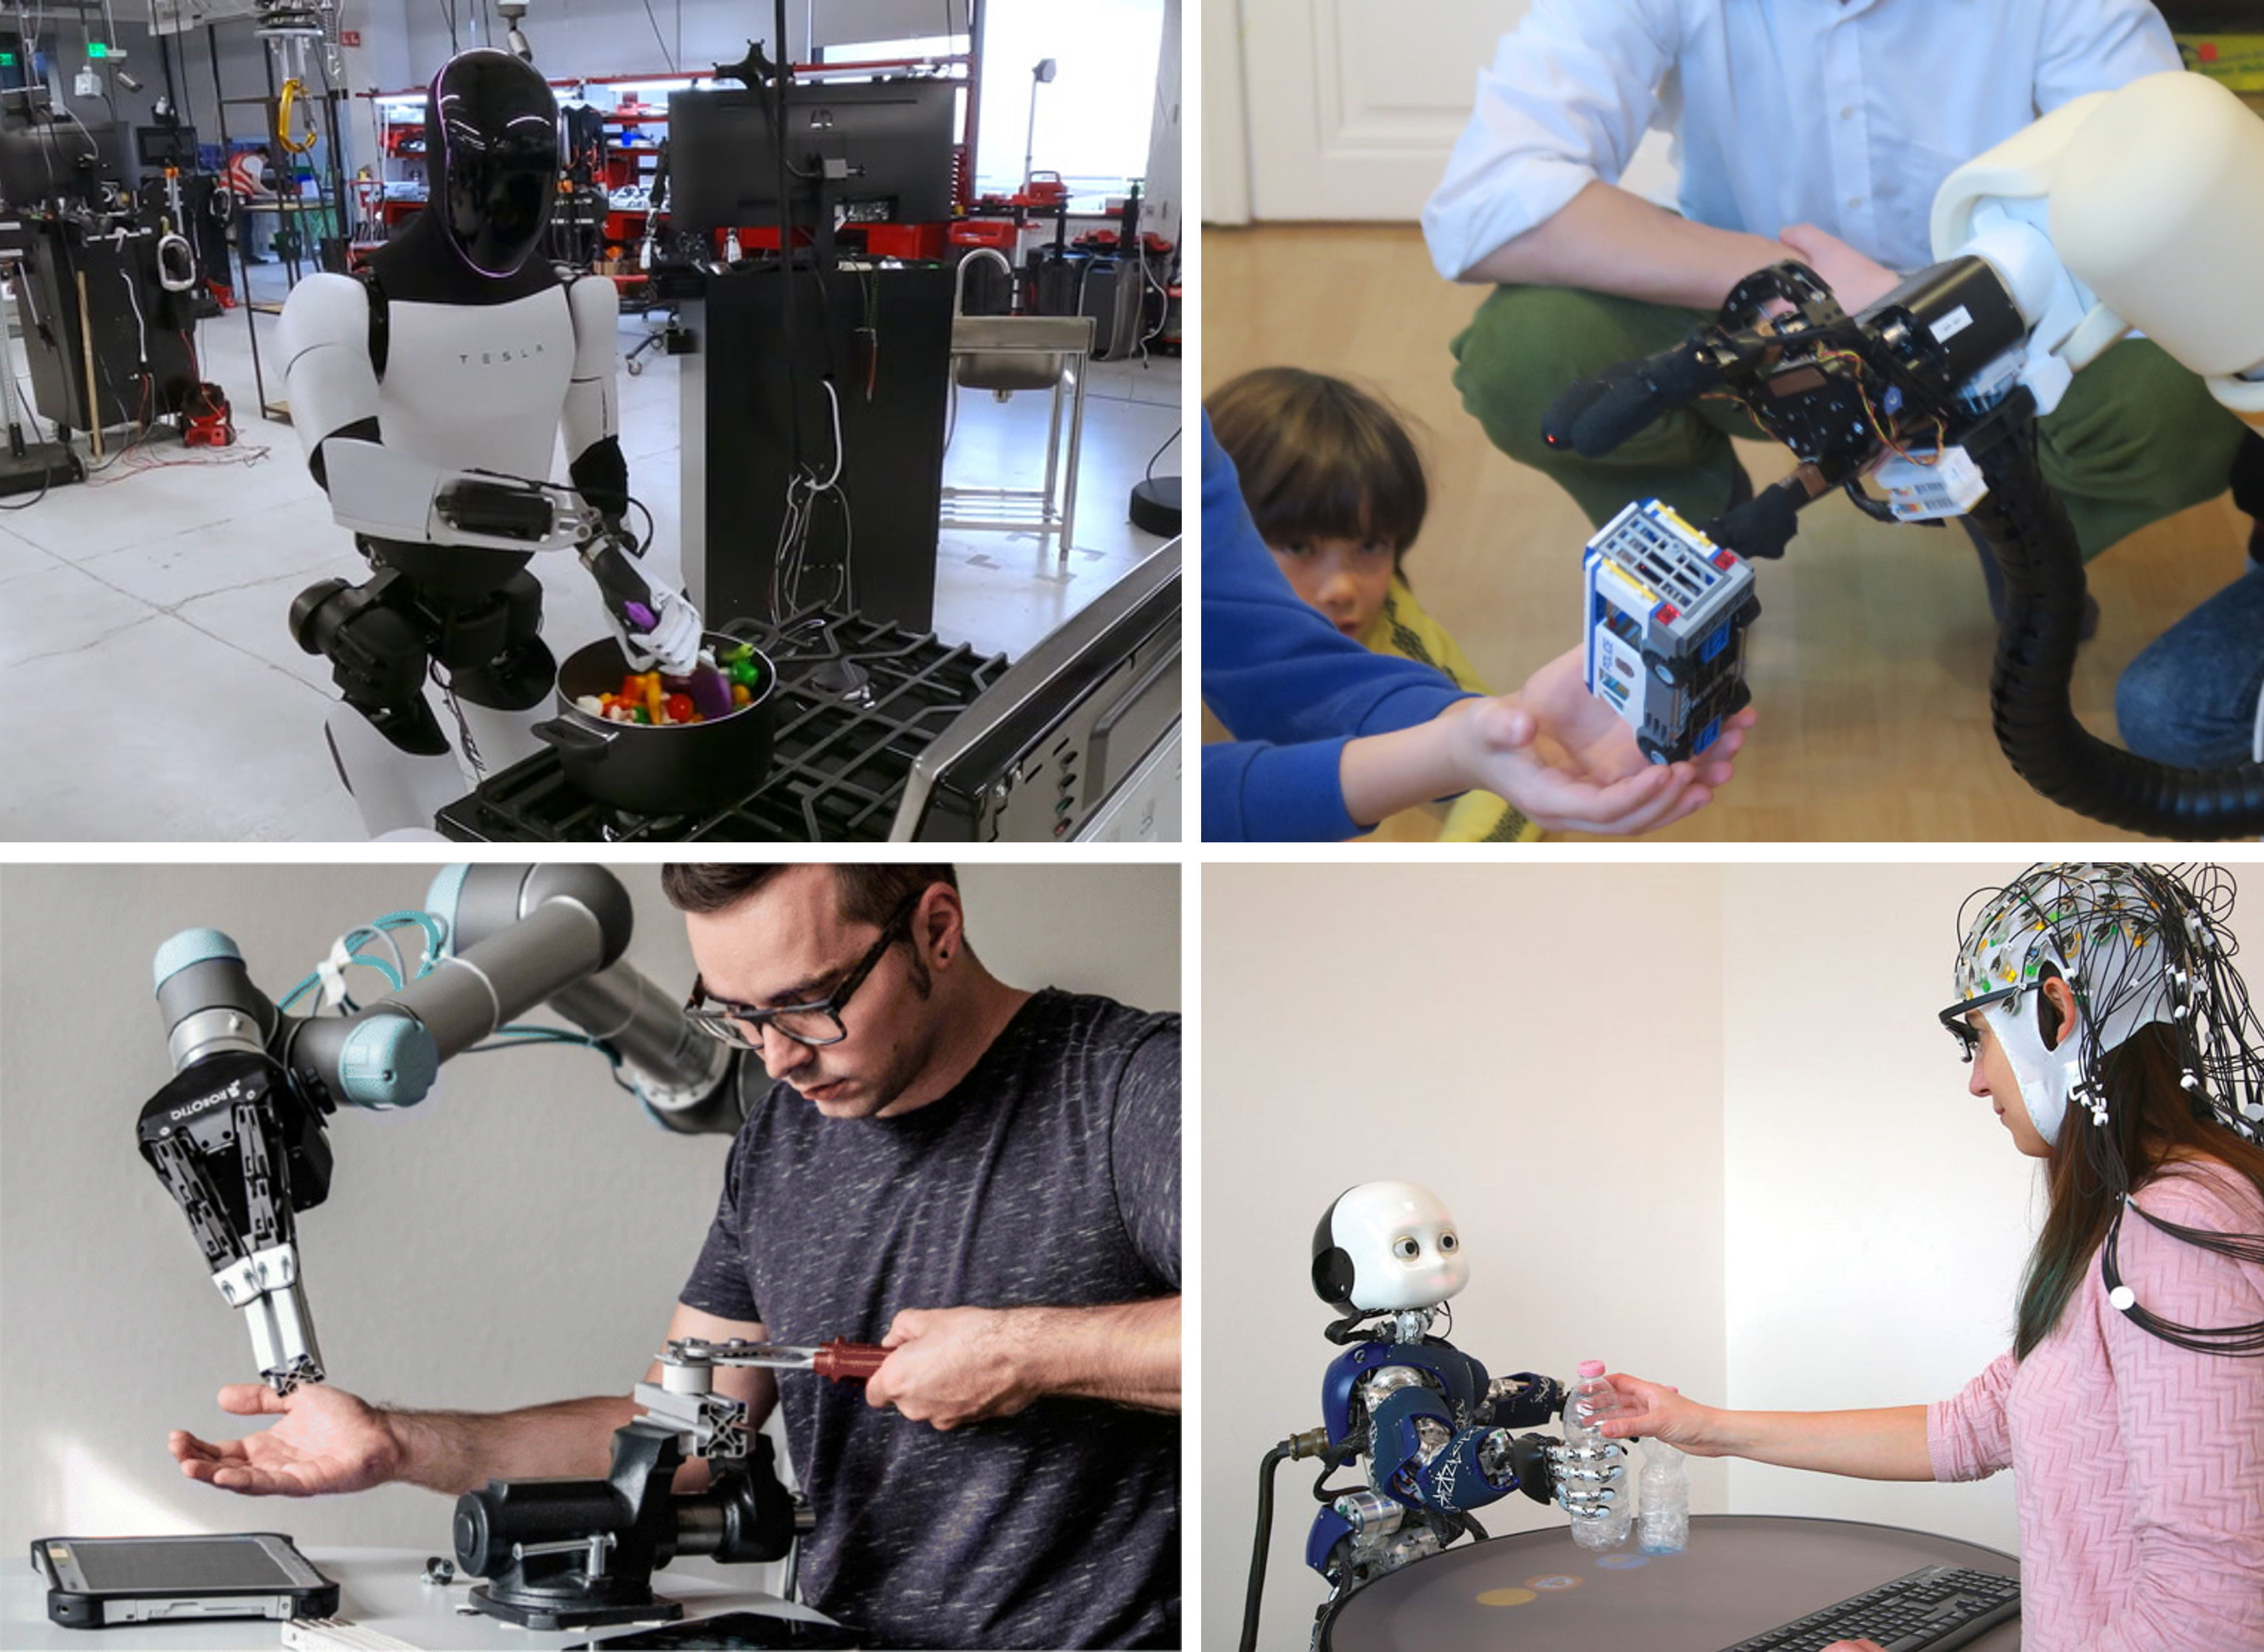
\includegraphics[width=0.8\textwidth]{general1}}
 	\caption{ورود ربات ها به دنیای تعامل با انسان ها
 		%\cite{kim2016integrated}
 	}
 	\label{fig:general1}
 \end{figure}


\section{نحوه‌ی ادراک  ربات ها از محیط و اشیاء}
ربات‌ها به طور معمول از حسگرهای گوناگونی برای درک محیط استفاده می‌کنند. این حسگرها را می‌توان به دو دسته  کلی غیرتماسی و تماسی تقسیم کرد. انواع دوربین های دوبعدی، تشخیص عمق و رادار لیزری
\LTRfootnote{LIDAR}
نمونه‌ای از حسگرهای غیرتماسی هستند که اطلاعاتی در مورد اشیاء و محیط، بدون تماس فیزیکی، فراهم می‌کنند. این حسگرها به در خدمت روش های یادگیری ماشین، توانسته‌اند ربات‌ها را قادر سازند تا برنامه‌ریزی صحیحی برای تعامل با محیط انجام دهند و محل مناسب برای گرفتن اشیاء را تشخیص دهند.
\cite{tian2023data,hosseini2024multi,beigy2024explorable,sabzejou20232d,moghadam2023grasp}
\subsection{آیا بینایی به تنهایی کافیست؟}

با وجود پیشرفت‌های چشمگیر در حوزه‌ی بینایی ماشین
\LTRfootnote{Computer Vision}
و کنترل ربات بر مبنای این حس
\LTRfootnote{Vision-based Robot Control}
،بینایی به تنهایی برای انجام وظایف پیچیده کافی نبوده و قادر به درک ویژگی‌های فیزیکی اشیا مانند نرمی، شکنندگی، بافت سطح یا نیروی اعمالی نیست. حس بینایی نمی‌تواند به طور مستقیم و در لحظه اصطکاک و یا لغزش بین چنگک و جسم را تشخیص دهد؛ با تکیه بر بینایی نمی‌توان میزان نیروی اعمال شده به یک جسم نرم یا شکننده را کنترل کرد.
\cite{yamaguchi2019recent,chi2018recent}
همچنین، هنگامی که چنگک
\LTRfootnote{Gripper}
 یک جسم را می‌گیرد، آن جسم ممکن است دید حسگر بینایی را مسدود کند و اطلاعات لحظه‌ای مربوط به تماس از دست برود. این ناتوانی‌ها چالشی بزرگ برای تعامل پایدار و مفید با اشیاء ایجاد می‌کنند. در نتیجه واضح است که صرفاً اتکا به حس بینایی برای انجام وظایف پیچیده و ظریف کافی نیست و نیاز به اطلاعات حسی دیگری به‌ خصوص حس لامسه ضروری است.
\subsection{لزوم حس لامسه در ربات}
حس لامسه یکی از مؤلفه‌های اصلی برای درک محیط توسط ربات، به‌ویژه در تعامل فیزیکی با اشیا، است. این حس امکان اندازه‌گیری نیروهای عمودی و جانبی، تشخیص برخورد با سایر عوامل موجود در محیط واعمال نیروی مناسب در حین انجام وظایف را فراهم می‌کند.
\cite{zou2017novel, yousef2011tactile}
وجود حس لامسه برای انجام وظایفی که نیازمند کنترل دقیق نیرو و تعامل ایمن با اشیای ظریف هستند، ضروری است. به عنوان مثال، در وظایف مونتاژ، جابه‌جایی مواد غذایی، یا تعامل با انسان، حس لامسه نقشی کلیدی در جلوگیری از آسیب به اشیا و بهبود عملکرد کلی ایفا می‌کند.
همچنین، پژوهش‌ها نشان داده‌اند که ادغام داده‌های لامسه و بینایی می‌تواند ادراک ربات را مشابه عملکرد انسان بهبود و سازگاری ربات با شرایط ناشناخته را افزایش دهد.
\cite{dahiya2013robotic}

\subsection{اهمیت حس لامسه در چنگک های رباتی}
عملگرهای نهایی 
\LTRfootnote{End-Effectors}
و به‌ویژه چنگک‌ها، اصلی‌ترین رابط مکانیکی بین ربات و محیط پیرامون آن محسوب می‌شوند. آن‌ها نقطه اصلی تماس ربات با اشیاء هستند و بخش عمده‌ای از وظایف یک ربات، از جمله گرفتن، جابجایی و دستکاری اشیاء، توسط این ابزارها انجام می‌شود. در دهه‌های گذشته، تمرکز اصلی در رباتیک صنعتی بر روی وظایف تکراری و از پیش تعریف‌‌شده در محیط‌های کاملاً کنترل‌شده بود؛ اما امروزه با گسترش کاربرد ربات‌ها در حوزه‌هایی مانند خدمات، پزشکی، کشاورزی و تعامل مستقیم با انسان، نیاز به ساختاری امن، قابل اعتماد و هوشمند برای این تعاملات به یکی از اهداف اصلی حوزه رباتیک تبدیل شده است.
\cite{broadbent2017interactions}
عملکرد قابل اطمینان برای چنگک‌های رباتی بسیار فراتر از یک گرفتن و رها کردن ساده است. یک گرفتن موفق نه تنها مستلزم لمس جسم هدف می‌باشد، بلکه باید از خطراتی مانند لغزش
\LTRfootnote{Slippage}
  شئ هدف و یا آسیب رساندن به آن به دلیل اعمال نیروی بیش از حد نیز جلوگیری شود. اینجاست که محدودیت‌های سیستم‌های کنترلی که صرفاً بر حس بینایی متکی هستند، آشکار می‌شود. اگرچه بینایی در مراحل اولیه مانند شناسایی و مکان‌یابی شیء نقشی حیاتی دارد، اما در لحظه تماس فیزیکی، به دلیل انسداد دید توسط خود چنگک و عدم توانایی درک خواص فیزیکی نامشهود، کارایی خود را از دست می‌دهد.
 \cite{malis2002survey}
 \\
 وجود حس لامسه در چنگک‌ها، این شکاف اطلاعاتی را پر کرده و کلید دستیابی به دستکاری 
 \LTRfootnote{Manipulation}
 پایدار، دقیق و هوشمند است. حسگرهای لامسه با فراهم آوردن اطلاعات بی‌درنگ از شرایط تماس، قابلیت‌های چنگک را به شکل چشمگیری افزایش می‌دهند. چند نوع از اطلاعاتی که حسگرهای لامسه می‌توانند فراهم کنند، شامل موارد زیر می‌شود:
 \begin{itemize}
 	\item \textbf{اندازه‌گیری نیرو و گشتاور } 
 	\\
حسگرهای لامسه می‌توانند مقادیر دقیق نیروهای نرمال و برشی اعمال‌شده بر سطح شیء را اندازه‌گیری کنند. این اطلاعات به سیستم کنترل اجازه می‌دهد تا نیروی گرفتن را به طور پیوسته تنظیم کند؛ نیروی اعمالی نباید آن‌قدر زیاد باشد که به جسم آسیب بزند و در عین حال، نباید آن‌قدر کم باشد که جسم بلغزد و از دست ربات رها شود
 	\cite{piga2023adaptive}
 	. توانایی انسان در بلند کردن یک تخم‌مرغ بدون شکستن آن، مثال بارزی از همین تنظیم دقیق نیرو بر اساس بازخورد لمسی است.
 	 
 	 \item \textbf{تشخیص لغزش} 
 	 \\
لغزش یکی از پدیده‌های دینامیکی کلیدی در حین دستکاری اشیاء است. حسگرهای لامسه، به‌ویژه آن‌هایی که به ارتعاشات فرکانس بالا حساس هستند، می‌توانند شروع لغزش را در مراحل اولیه تشخیص دهند. این تشخیص زودهنگام به کنترل‌کننده ربات فرصت می‌دهد تا به سرعت نیروی گرفتن را افزایش داده و از افتادن شیء جلوگیری کند.
 	 \cite{kyberd2023slip,costanzo2018slipping}
 	 
 	 \item \textbf{شناسایی موقعیت و توزیع تماس}
آرایه‌ای از حسگرهای لامسه می‌تواند نقشه‌ای از توزیع فشار بر روی سطح انگشتان چنگک ربات ایجاد کند. این اطلاعات برای تعیین مرکز فشار، تشخیص جهت‌گیری شیء در دست و اطمینان از یک گرفتن پایدار بسیار ارزشمند است.
\cite{khamis_novel_2019,de2022soft,wang_low-cost_2016}
\\
 \begin{figure}[ht]
	\centerline{\includegraphics[width=0.8\textwidth]{general2}}
	\caption{نمونه‌ای از تعامل چنگک های رباتی با اشیاء ظریف و نرم
		\cite{zhang2020state}
	}
	\label{fig:general1}
\end{figure}
 \end{itemize} 
\subsection{الهام از زیست: حس لامسه در انسان}
طبیعت در طول میلیون‌ها سال فرگشت، سیستم‌های بهینه‌ای را برای تعامل با محیط فیزیکی توسعه داده است. در میان این سیستم‌ها، حس لامسه انسان به عنوان پیچیده‌ترین، کارآمدترین و چندوجهی‌ترین سیستم حسی برای تعامل یا اشیاء شناخته می‌شود. پوست انسان، به‌ویژه در ناحیه نوک انگشتان، یک شاهکار مهندسی بیولوژیک است که ترکیبی از حساسیت بالا، استحکام، قابلیت ترمیم و توانایی پردازش اطلاعات پیچیده را به نمایش می‌گذارد. به همین دلیل، درک عمیق سازوکار حس لامسه انسان، نه تنها الهام‌بخش، بلکه یک نقشه راه ضروری برای طراحی و ساخت  حسگرهای رباتیکی است. 
\cite{silvera2015artificial}
موفقیت سیستم لامسه انسان در دستیابی به تعامل ماهرانه
\LTRfootnote{Dexterous Manipulation} 
 بر دو اصل بنیادین استوار است که در این پژوهش نیز به عنوان انگیزه اصلی مورد توجه قرار گرفته‌اند: 
 \textbf{اهمیت چندوجهی بودن ادراک حسی و ویژگی نرم و ارتجاعی نوک انگشتان.}
 در ادامه این بخش، این دو اصل کلیدی با جزئیات بیشتری بررسی می‌شوند.
\subsubsection{ ماهیت چندوجهی حس لامسه انسان}

پوست انسان یک حسگر یکپارچه و همگن نیست، بلکه مجموعه‌ای از گیرنده‌های حسی تخصصی است که هرکدام به نوع خاصی از محرک‌های لمسی با پهنای باند متفاوت پاسخ می‌دهند. این گیرنده‌های مکانیکی
 \LTRfootnote{Mechanoreceptors}
 که مسئول تبدیل محرک‌های لمسی به سیگنال‌های عصبی هستند، عمدتاً در لایه‌های روپوست
 \LTRfootnote{Epidermis}
و لایه‌ی میانی
\LTRfootnote{Dremis}
قرار دارند. در پوست بدون مو  مانند نوک انگشتان، که برای تعامل با اشیاء تکامل یافته‌اند، چهار نوع اصلی گیرنده مکانیکی وجود دارد که هر یک وظیفه مشخصی بر عهده دارند.
 \cite{wettels2011biomimetic, chi2018recent}.
\\
\begin{figure}[t]
	\centering
	\centerline{\includegraphics[width=0.8\textwidth]{Human_skin}}
	\caption{مقطعی از ساختار پوست انسان و محل قرارگیری چهار گیرنده لامسه اصلی در نوک انگشتان
		\cite{silvera2015artificial}
		. }
	\label{fig:skin_cross_section}
\end{figure}
این چهار گیرنده بر اساس سرعت پاسخشان به محرک‌های لامسه، به دو دسته اصلی تقسیم می‌شوند. دسته اول، گرینده های فرکانس پایین هستند که تا زمانی که محرک فیزیکی وجود داشته باشد، به طور پیوسته سیگنال عصبی تولید می‌کنند و مسئول درک اطلاعات استاتیک مانند نیرو هستند. دسته دوم، گیرنده های فرکانس بالا می‌باشند که فقط به تغییرات در محرک فیزیکی، یعنی در لحظه شروع و پایان تماس، پاسخ می‌دهند؛ این گروه مسئول درک اطلاعات دینامیک و گذرا هستند. این تقسیم‌بندی، اساس توانایی انسان در درک همزمان نیروهای مانا و پدیده‌های دینامیکی مانند لغزش است.
\begin{table}[ht]
	\caption{خلاصه‌ای از ویژگی‌ها و وظایف گیرنده‌های لامسه در نوک انگشتان انسان
\cite{chi2018recent}	
.}
	\label{tab:mechanoreceptors}
	\centering
	\onehalfspacing
	\begin{tabular}{|r|r|r|r|}
		\hline
		\textbf{نام گیرنده} & \textbf{محدوده فرکانس (هرتز)} &  \textbf{وظیفه اصلی} & \textbf{معادل در رباتیک} \\
		\hline \hline
		دیسک‌های مرکل
		\footnotemark
		
		 &  ۰.۳ - ۳ & فشار استاتیک&  نیروی گرفتن \\
		پایانه‌های رافینی
		\footnotemark
		 &  تا ۱۵ & کشش پوست، & نیروی مماسی\\
		گویچه‌های مایسنر
		\footnotemark
		 & ۳ - ۴۰ & تماس اولیه، لغزش آرام & تشخیص رویداد تماس \\
		گویچه‌های پاچینی 
		\footnotemark
		& ۱۰ - ۵۰۰ & ارتعاشات، لغزش  & تشخیص لغزش \\
		\hline
	\end{tabular}
\end{table}
\LTRfootnotetext[13]{Merkel's disks}
\LTRfootnotetext[14]{Ruffini's corpuscles}
\LTRfootnotetext[15]{Meissner corpuscles}
\LTRfootnotetext[16]{Pacinian corpuscles}
\\
این «تفکیک وجه ها» به مغز اجازه می‌دهد تا اطلاعات غنی و متنوعی را به صورت موازی پردازش کند و این همان اصلی است که این پژوهش با طراحی و ساخت یک حسگر چندوجهی
\LTRfootnote{Multi-modal}
قصد پایبندی به آن را دارد.
این تقسیم‌بندی پیچیده نشان می‌دهد که چرا تلاش برای ساخت یک حسگر لامسه رباتیک با تنها یک نوع تبدیل (مثلاً فقط اندازه‌گیری فشار) برای دستیابی به مهارت انسان کافی نیست. یک حسگر لامسه زیست الهام
\LTRfootnote{Biomimetic}
 واقعی باید بتواند اطلاعات استاتیک و دینامیک را در پهنای باندهای مختلف به صورت همزمان دریافت و پردازش کند
 \cite{silvera2015artificial}.
  این دقیقاً همان هدفی است که در این پژوهش با ترکیب یک حسگر فشار بارومتریک (برای درک اطلاعات استاتیک مشابه مرکل)، حسگرهای اثر هال (برای درک کشش و نیروی برشی مشابه رافینی)، حسگر دما و یک میکروفون (برای درک ارتعاشات فرکانس بالا مشابه پاچینی) دنبال شده است.


\subsubsection{ویژگی نرم و ارتجاعی نوک انگشتان}

دومین اصل کلیدی در موفقیت حس لامسه انسان، ماهیت فیزیکی خود انگشتان است. نوک انگشتان انسان از بافت نرم و ارتجاعی ساخته شده است که این ویژگی مزایای مکانیکی مهمی را در حین تعامل با اشیاء فراهم می‌کند.
یکی از مهم‌ترین این مزایا، \textbf{افزایش سطح تماس و پایداری گرفتن} است. هنگامی که یک انگشت نرم با یک جسم تماس پیدا می‌کند، تغییر شکل داده و خود را با شکل سطح جسم تطبیق می‌دهد. این امر باعث افزایش قابل توجه سطح تماس در مقایسه با یک انگشت صلب می‌شود. سطح تماس بزرگتر، نیروی گرفتن را بر روی ناحیه وسیع‌تری توزیع می‌کند که این امر اولاً خطر آسیب به اشیاء شکننده را کاهش می‌دهد و ثانیاً با افزایش مقاومت در برابر گشتاورهای خارجی، یک گرفتن بسیار پایدارتر ایجاد می‌کند
 \cite{yousef2011tactile}.

علاوه بر این، نرمی انگشتان بسیاری از عدم قطعیت‌ها و خطاهای کوچک در مکان‌یابی و جهت‌گیری شیء را جبران می‌کند. نیازی نیست که ربات موقعیت دقیق جسم را بداند؛ بافت نرم انگشت، خود را با ناهمواری‌ها و شکل‌های نامنظم تطبیق می‌دهد و یک تماس کامل را تضمین می‌کند. این ویژگی، نیاز به الگوریتم‌های کنترلی پیچیده را کاهش داده و به گرفتن قابل اطمینان کمک می‌کند.

نهایتاً، این تغییرشکل‌پذیری منجر به تقویت سیگنال‌های لمسی می‌شود. تغییر شکل پوست در اطراف یک شیء، الگوهای فشار و کشش منحصربه‌فردی را بر روی گیرنده‌های مکانیکی زیرین ایجاد می‌کند. به عنوان مثال، لبه‌های یک جسم باعث ایجاد تمرکز تنش در پوست می‌شوند که این امر به گیرنده‌های مرکل کمک می‌کند تا شکل را با دقت بیشتری تشخیص دهند. این پدیده به ربات نیز کمک می‌کند تا اطلاعات غنی‌تری از تماس استخراج کند.
\cite{silvera2015artificial}
این مزایا نشان می‌دهد که طراحی یک حسگر لامسه موفق، تنها به انتخاب مبدل‌های الکترونیکی مناسب محدود نمی‌شود، بلکه به طراحی مکانیکی و مواد به کار رفته در ساختار آن نیز بستگی دارد. استفاده از مواد نرم مانند سیلیکون در ساخت حسگرهای رباتیک، تلاشی برای تقلید از این ویژگی‌های سودمند فیزیکی انگشتان انسان است.

در نتیجه، با الهام از این دو اصل، این  پژوهش نه تنها بر توسعه یک سیستم الکترونیکی چندوجهی تمرکز داشته، بلکه این سیستم را در یک ساختار نرم و ارتجاعی ادغام می‌کند تا به ترکیبی بهینه از درک حسی و سازگاری مکانیکی، مشابه دست انسان، دست یابد.

\section{انواع روش های تبدیل در ساخت حسگر لامسه و مروری بر کار‌های پیشین}
\subsection{روش های مبتنی بر پیزوالکتریک}

از منظر لغوی، پیزو به معنی فشار است و ترکیب پیزو الکتریک
\LTRfootnote{Piezo-electric}
 به موادی اطلاق می‌شود که در اثر اعمال فشار، سیگنال الکتریکی از خود تولید می‌کنند. این حسگر‌ها از پدیده‌ای فیزیکی به نام اثر پیزوالکتریک بهره می‌برند. این اصطلاح علمی به معنای «الکتریسیته ناشی از فشار» است و به توانایی برخی مواد خاص برای تولید یک ولتاژ یا بار الکتریکی در پاسخ به کرنش مکانیکی یا فشار اشاره دارد. ساختار بلوری این مواد به گونه‌ای است که در حالت عادی، بارهای مثبت و منفی به طور متقارن توزیع شده و اثر یکدیگر را خنثی می‌کنند، اما با اعمال فشار یا نیروی مکانیکی، این تقارن به هم می‌خورد و بارهای الکتریکی مثبت و منفی در دو طرف ماده ظاهر می‌شوند، که منجر به تولید یک ولتاژ قابل اندازه‌گیری می‌گردد. این پدیده در موادی مانند کریستال‌های کوارتز 
\LTRfootnote{Quartz crystals}،
 سرامیک‌های پیزوالکتریک مانند PZT
 \LTRfootnote{Lead Zirconate Titanate}
  و برخی پلیمرها مانند PVDF
 \LTRfootnote{Polyvinylidene Fluoride}) مشاهده می‌شود.
\\
برای کاربردهای حسگر لامسه، مواد پیزوالکتریک به دلیل ویژگی‌های منحصربه‌فردشان بسیار مناسب هستند. این حسگرها نیازی به منبع تغذیه خارجی ندارند و می‌توانند به صورت فعال
\LTRfootnote{Active}
 عمل کنند که این ویژگی، مصرف انرژی را به شدت کاهش می‌دهد. مهم‌ترین مزیت این مکانیزم، پاسخ دینامیکی فوق‌العاده سریع و حساسیت بسیار بالا به تغییرات نیرو است. این خصوصیت آن‌ها را برای تشخیص ارتعاشات با فرکانس بالا و لغزش‌های بسیار جزئی
 \LTRfootnote{Micro-Slip}
 ایده‌آل می‌کند. در واقع، یک حسگر پیزوالکتریک می‌تواند لغزش یک جسم را در کسری از ثانیه تشخیص دهد که این امر به ربات اجازه می‌دهد قبل از افتادن کامل شیء، نیروی عمودی را اصلاح کند. پژوهش های متعددی در این زمینه انجام شده‌است که به ساخت حسگرهای لامسه پیزوالکتریک برای کاربردهای مختلف پرداخته‌اند. برای مثال، در پژوهش 
\cite{nasserii2011Piezo}
  نویسندگان به طراحی و ساخت یک حسگر بر اساس تغییر امپدانس کریستال پیزوالکتریک برای اندازه‌گیری نیروی اعمالی می‌پردازد. این حسگر با سنجش ولتاژ خروجی ناشی از فشار، توانایی تخمین نیروی اعمال شده را دارد. نتایج این پژوهش نشان داد که با توجه به طراحی ساده، حسگر ساخته شده قابلیت تغییر اندازه و شکل را دارد و برای کاربردهایی مانند جراحی‌های کم‌تهاجمی مناسب است. با این حال، جزئیات دقیق و کمی از دقت و حساسیت آن ارائه نشده است.
  همچنین،
  \cite{spanu2016PVDF}
   یک حسگر لمسی بسیار حساس را معرفی می‌کنند که از یک پلیمر پیزوالکتریک (PVDF) به همراه ترانزیستور ارگانیک استفاده می‌کند و برای پوست رباتیک مطرح شده است. حسگر مذکور توانایی اندازه‌گیری نیروهایی که به کوچکی 20mN را دارد.
   در مقاله‌ی 
   \cite{qi2023PVDF}
نویسندگان به بررسی انواع مواد قابل استفاده برای طراحی حسگر لامسه مبتنی بر پیزوالکتریک می‌پردازند.
    پژوهش‌هایی مانند
 \cite{wang2019PiezoArray,huang2024piezo,yu2016PiezoArray}
   به ساخت آرایه‌های حسگر پیزوالکتریک انعطاف‌پذیر برای اندازه‌گیری نیروهای سه‌محوری و تشخیص لغزش در حین گرفتن اشیاء پرداخته اند. سرعت خوانش اطلاعات در این پژوهش‌ها 5 تا 400 هرتز و در 
   \cite{huang2024piezo}
   1900 هرتز می‌باشد. بازه‌ی اندازه‌گیری نیرو به ترتیب 15، 11 و \LR{1.5} نیوتن برای محور عمودی گزارش شده است.
   
\begin{figure}[t]
	\centering
	\includegraphics[width=0.8\textwidth]{wang_piezo}
	\caption{شمای کلی حسگر ارائه شده در پژوهش 
		\cite{wang2019PiezoArray}
		. }
	\label{fig:wang_piezo}
\end{figure}
   
\begin{table}[ht]
	\centering
	\caption{مقایسه سنسورهای لمسی پیزوالکتریک گزارش‌شده در مقالات مختلف}
	\label{tab:piezo_sensors}
	\onehalfspacing
	\begin{tabular}{|r|r|r|r|r|r|}
		\hline
		\textbf{مرجع} & \textbf{سال} & \textbf{تعداد المان‌های حسی}  & \textbf{بازه نیرو} & \textbf{حساسیت} & \textbf{ماده پیزوالکتریک} \\ \hline \hline
		
		\cite{nasserii2011Piezo} & 2011 & 1 &$12 \: N$ & $33.47 \frac{mV}{N}$ & سرامیک پیزو \\ \hline
		
		\cite{spanu2016PVDF} & 2016 & 1 & 
		 $3.5 \: N$ & $3 \frac{nA}{N}$ & PVDF + Organic transistor \\ \hline
		
		\cite{yu2016PiezoArray} & 2016 & $2 \times 3 $ & $1.5 \: N$ & 
		$6.62 \frac{pC}{N}$ & \LR{PVDF} \\ \hline
		
		\cite{wang2019PiezoArray} & 2019 & $3 \times 3 $& $15 \: N$ &  $210 \frac{mV}{N}$ & PVDF \\ \hline
		
		\cite{huang2024piezo} & 2024 &$ 3‌ \times 3 $& $11 \: N$ & $35.6 \frac{mV}{N}$ & PVDF-based (rigid-in-soft) \\ \hline
		
	\end{tabular}
\end{table}

\subsection{روش های مبتنی بر پیزو مقاومت}
مکانیزم پیزومقاومتی یکی از بنیادی‌ترین و پرکاربردترین اصول در طراحی حسگرهای لامسه است که در سال‌های اخیر با توسعه مواد پیشرفته و ساختارهای میکرو و نانومتری توجه بسیاری را به خود جلب کرده است. اساس این روش بر این واقعیت استوار است که مقاومت الکتریکی یک ماده رسانا یا نیمه‌رسانا تحت تأثیر تغییرات مکانیکی نظیر فشار، کشش یا خمش تغییر می‌کند. این تغییر مقاومت را می‌توان به‌صورت یک سیگنال الکتریکی خواند و متناسب با آن شدت یا نوع تحریک مکانیکی را تعیین نمود. در واقع، تحریک مکانیکی به‌طور غیرمستقیم به یک پاسخ الکتریکی تبدیل می‌شود و همین امر امکان استفاده از آن را در ساخت پوست‌های مصنوعی، پروتزهای هوشمند و ربات‌های دارای قابلیت حس لامسه فراهم می‌سازد.

از دیدگاه فیزیکی، تغییرات مقاومت الکتریکی در یک ماده‌ی پیزو دو منشاء می‌تواند داشته باشد؛ منشاء اول تغییرات هندسی ماده مذکور است. همان‌طور که در رابطه‌ی کلاسیک مقاومت 
\begin{equation}\label{eq:piezoRes1}
	R=\rho\frac{l}{A}
\end{equation}
​

دیده می‌شود، اعمال تنش باعث افزایش طول و کاهش سطح مقطع یک رسانا می‌گردد و در نتیجه مقاومت آن تغییر می‌کند. دلیل دوم به تغییر مقاومت ویژه یا همان مقاومت ذاتی ماده مربوط است. در نیمه‌رساناهایی مانند سیلیکون و ژرمانیم، تنش مکانیکی موجب تغییر ساختار باند انرژی می‌شود و این تغییر، تحرک بارهای الکتریکی و چگالی آنها را دگرگون کرده و در نهایت مقاومت ویژه را تغییر می‌دهد
\begin{figure}[ht]
	\centering
	\includegraphics[width=0.8\textwidth]{piezoRes_ahmed2013mems}
	\caption{المان پیزومقاومتی استفاده شده در
		\cite{ahmed2013piezores}
		از جنس
		\LR{Si3N4 }}
		\label{fig:ahmed_piezores}
	\end{figure}
	. علاوه بر این دو منشاء، در ترکیباتی که شامل نانومواد کربنی، نانوسیم‌های فلزی یا ذرات رسانا هستند، تغییر مقاومت بیشتر ناشی از تغییر در مقاومت تماسی میان ذرات و پدیده‌هایی مانند تونل‌زنی کوانتومی
	\LTRfootnote{Quantum Tunneling Effect}
	است. زمانی که فشار به چنین ساختارهایی اعمال می‌شود، فاصله میان ذرات کاهش یافته و تماس‌های الکتریکی جدیدی ایجاد می‌شود که این فرایندها تغییرات شدیدی در مقاومت الکتریکی ایجاد می‌کنند.
	\cite{xi2024mechanisms}

	
	\begin{figure}[ht]
		\centering 
		\subfloat[مقوامت الکتریکی نسبت به نیرو\cite{drimus2014piezores}]{ \label{fig:pizeoResplots:RF}
			\includegraphics[width=0.5\textwidth]{drimus_2014_RF}}
		%\hspace{2mm}
		\subfloat[پسماند الکتریکی هنگام اعمال و برداشتن نیرو\cite{koiva2013piezores}]{ \label{fig:pizeoResplots:hysteresis}
			\includegraphics[width=0.5\textwidth]{koiva2013_piezoHysteresis}}%
		\caption{نمودارهای مشخصه برای حسگر های پیزومقاومتی.
		\ref{fig:pizeoResplots:RF}: مقاومت الکتریکی بر حسب نیرو.
	\ref{fig:pizeoResplots:hysteresis}پسماند سیگنال
\cite{koiva2013piezores}}
		\label{fig:pizeoResplots} %% label for entire figure
	\end{figure}
	
	
	
	پژوهش‌های متعددی برای بهبود حساسیت و محدوده‌ی عملکرد حسگرهای پیزومقاومتی انجام شده است. به عنوان نمونه، پژوهشگران در
	\cite{jing2022ag} 
	یک حسگر پیزومقاومتی انعطاف‌‌پذیر مبتنی بر نانوسیم‌های نقره و 
	\LR{PVDF}
	توسعه دادند که دارای ساختار سه‌بعدی متخلخل بود و به دلیل توزیع یکنواخت نانوسیم‌ها، حساسیت مناسبی در بازه ۰ تا ۱۰۰ کیلوپاسکال به دست آورد.  
	
	نمونه‌ی دیگر، پژوهش \cite{zhao2022pdms} است که از ترکیب نانولوله‌های کربنی و گرافن روی بستر
	\LR{PDMS}\LTRfootnote{Poly dimethyl siloxane}
	متخلخل استفاده کردند. آنها با ایجاد میکروحفره‌های یکنواخت در بستر از طریق گرمایش مایکروویوی، سطح تماس بسیار زیادی برای نانومواد رسانا فراهم آوردند. نتیجه این طراحی، دستیابی به حساسیتی در حدود \(300.31 \, kPa^{-1}\) در فشارهای پایین (۰ تا ۵۰ کیلوپاسکال) بود.  
	
	مکانیزم پیزومفاومتی محدودیت هایی نیز دارد؛ به طور مثال در شکل
	\ref{fig:pizeoResplots:RF}
	مشاهده می‌شود که رفتار غیرخطی حسگر در بازه‌های وسیع فشار باعث می‌شود رابطه بین نیروی واردشده و تغییر مقاومت همیشه خطی نبوده و کالیبراسیون دقیق را دشوار می‌سازد.
	علاوه بر این، با توجه به شکل 
	\ref{fig:pizeoResplots:hysteresis}
	وجود پسماند
	\LTRfootnote{Hysteresis}
	در پاسخ حسگر باعث می‌شود که مقادیر خروجی در هنگام اعمال و برداشت نیرو یکسان نباشد و دقت اندازه‌گیری کاهش یابد. عامل دیگر، حساسیت بالا به تغییرات دما است، زیرا افزایش دما می‌تواند تحرک حامل‌های بار و نیز مقاومت ویژه ماده را تغییر دهد و در نتیجه پاسخ حسگر را تحت تأثیر قرار دهد. همچنین این دسته از حسگرها اغلب دارای زمان بازیابی طولانی پس از اعمال نیرو هستند، به این معنا که بازگشت به حالت اولیه در بسیاری از طراحی‌ها به کندی صورت می‌گیرد. این ویژگی‌ها موجب محدودیت در استفاده از حسگرهای پیزومقاومتی در محیط‌هایی با تغییرات سریع نیرو یا دما شده و پژوهشگران را به سمت توسعه راهکارهای جبرانی، طراحی ترکیبی با مکانیزم‌های دیگر و استفاده از مواد نوین سوق داده است.
	
	
	\begin{table}[ht]
		\centering
		\caption{مقایسه سنسورهای لمسی پیزومقاومتی گزارش‌شده در مقالات مختلف}
		\label{tab:piezo_res}
		\onehalfspacing
		\begin{tabular}{|r|r|r|r|r|r|}
			\hline
			\textbf{مرجع} & \textbf{سال} & \textbf{تعداد المان‌های حسی}  & \textbf{بازه نیرو} & \textbf{حساسیت} & \textbf{ماده پیزوالکتریک} \\ \hline \hline
			
			\cite{noda2006cantilever} & 2006 & 1 &$-5 \: kPa - 5\: kPa (shear)$ & $0.03\%$ & Silicone \\ \hline
			
			\cite{koiva2013piezores} & 2013 & 12 & 
			$10 \: N$ & $0.015\%$ & LCPT\footnotemark \\ \hline
			
			\cite{ahmed2013piezores} & 2013 & $6 \times 8 $ & $30 \: kPa$ & 
			$1.25 \frac{V}{N}$ & \LR{Nichrome} \\ \hline
			
			\cite{drimus2014piezores} & 2014 & $8 \times 8 $ & $10 \: kPa$ & 
			$--$ & \LR{Conductive rubber} \\ \hline
			
			\cite{jing2022ag} & 2022 &$1$& $100 \: kPa$ &  $0.009 kPa^{-1} $ & AgNws + PVDF \\ \hline
			
			\cite{hou2022fiber} & 2022 &$ 1 $& $150 \: kPa$ & $2.06 kPa^{-1} $ & Cu + PDMS (rigid-in-soft) \\ \hline
			
			\cite{zhao2022pdms} & 2022 &$ 1$& $200 \: kPa$ & $300.31 kPa^{-1} $ & PDMS \\ \hline
		\end{tabular}
	\end{table}
	\LTRfootnote[30]{Liquid Crystal Polymer Thermoplastic}
	
\subsection{روش های خازنی}

فناوری خازنی یکی از پرکاربردترین و منعطف‌ترین رویکردها در طراحی حسگرهای لامسه رباتیک است. این حسگرها به دلیل حساسیت بالا، مصرف توان پایین و قابلیت مجتمع‌سازی در مقیاس بزرگ، توجه بسیاری از محققان را به خود جلب کرده‌اند. فلسفه اصلی در این حسگرها، اندازه‌گیری تغییر ظرفیت یک خازن بر اثر تغییر مکانیکی در ساختار و هندسه آن است. این حسگرها معمولاً از ساختاری شبیه به یک خازن صفحه‌موازی تشکیل شده‌اند که ظرفیت آن‌ها از طریق رابطه کلاسیک زیر محاسبه می‌شود:
\begin{equation}
	C=\frac{\varepsilon_0 \varepsilon_r A}{d}.
	\label{eq:basicC}
\end{equation}
در این رابطه، $C$ ظرفیت خازن، $\epsilon_0$ ثابت گذردهی خلأ، $\epsilon_r$ ثابت دی‌الکتریک نسبی ماده بین صفحات، $A$ سطح هم‌پوشانی صفحات و $d$ فاصله بین آن‌ها است. یک نیروی خارجی می‌تواند با تغییر پارامترهای هندسی \textbf{فاصله ($d$)} یا \textbf{سطح هم‌پوشانی ($A$)}، ظرفیت خازن را تغییر دهد و این تغییر، پس از اندازه‌گیری، به مقدار نیرو نگاشت می‌شود \cite{chi2018recent}.

اگرچه ساختار صفحه‌موازی اساس کار این حسگرهاست، اما طراحی‌های متنوعی برای اندازه‌گیری انواع مختلف نیرو (عمودی و برشی) و افزایش چشمگیر حساسیت توسعه یافته است.با این حال، متداول‌ترین مکانیزم، مبتنی بر \textbf{ساختار صفحه‌موازی برای نیروی عمودی} است. در این طراحی، یک لایه الاستومری نرم به عنوان ماده دی‌الکتریک بین دو الکترود رسانای انعطاف‌پذیر قرار می‌گیرد. هنگامی که یک نیروی عمودی به سطح حسگر وارد می‌شود، لایه الاستومری فشرده شده، فاصله $d$ بین صفحات کاهش می‌یابد و در نتیجه، ظرفیت خازن ($C$) به صورت غیرخطی افزایش پیدا می‌کند.

یک نوآوری کلیدی برای بهبود عملکرد این ساختار، استفاده از میکرو-ساختارها
\LTRfootnote{Micro-structures}
 در لایه دی‌الکتریک است. به جای استفاده از یک لایه صاف، الاستومر به شکل ساختارهای ریزی مانند هرم
\LTRfootnote{Pyramid}،
 گنبد 
 \LTRfootnote{Dome}
  یا ستون
  \LTRfootnote{Pillar}
   قالب‌گیری می‌شود \cite{mannsfeld2010highly}. این معماری هوشمندانه، نیرو را در نقاط کوچکی متمرکز کرده و باعث تغییر شکل بسیار بزرگتری در فاصله ($d$) به ازای یک فشار معین می‌شود. وجود فضاهای خالی در بین این میکرو-ساختارها باعث می‌شود حسگر در محدوده فشارهای پایین بسیار نرم و حساس عمل کند. در نتیجه، حساسیت حسگر فشار که به صورت زیر تعریف می‌شود:
  
  \begin{equation}
  	S = (\Delta C/C_0)/\Delta P
  	\label{eq:sensC}
  \end{equation}
     به شدت افزایش یافته و امکان تشخیص تماس‌های بسیار آرام را فراهم می‌آورد \cite{zou2017novel}.

علاوه بر روش ساخت، پیشرفت در علم مواد نیز تأثیر مستقیمی بر بهبود عملکرد، انعطاف‌پذیری و حساسیت حسگرهای خازنی داشته است. انتخاب لایه دی‌الکتریک نقشی حیاتی دارد؛ 
\LR{PDMS}
 به دلیل انعطاف ‌پذیری عالی، پایداری شیمیایی و زیست ‌سازگاری، یکی از محبوب‌ترین گزینه‌هاست. برای کاربردهایی که به نرمی بیشتری نیاز دارند، از الاستومرهایی مانند
 \LR{Ecoflex}
   نیز استفاده می‌شود. جهت افزایش بیشتر حساسیت، این پلیمرها گاهی با نانوذراتی با ثابت دی‌الکتریک بالا
 \LTRfootnote{High-k}
  مانند
  \LR{TiO₂} \LTRfootnote{Titanium dioxide}
    یا 
      \LR{BaTiO₃} \LTRfootnote{Barium titanate}
     ترکیب می‌شوند. این کار باعث افزایش ظرفیت اولیه خازن شده و تغییرات نسبی ظرفیت ($\Delta C/C_0$) را قابل توجه‌تر می‌سازد \cite{zou2017novel}.
     
برای آنکه کل حسگر انعطاف‌پذیر باشد، لایه‌های رسانا الکترودها نیز باید قابلیت تغییرشکل داشته باشند. به همین منظور، به جای لایه‌های فلزی صلب، از مواد رسانای انعطاف‌پذیر استفاده می‌شود. گزینه‌هایی مانند نانولوله‌های کربنی
\LTRfootnote{CNTs}، 
 گرافن
 \LTRfootnote{Graphene}، 
 پلیمرهای رسانا و حتی  فلز مایع مانند 
 \LR{EGaIn}\LTRfootnote{
 	Eutectic Gallium-Indium}
  به حسگر اجازه می‌ده دهند تا به راحتی خم شده و بر روی سطوح منحنی پیچیده‌ای مانند نوک انگشت  ربات نصب شوند \cite{chi2018recent}.


	\begin{figure}[t]
	\centering
	\includegraphics[width=0.8\textwidth]{capacitive1}
	\caption{ساختار حسگر لامسه خازنی معرفی شده در
		\cite{pagoli2022large}.}
	\label{fig:CapStructure}
\end{figure}

با وجود مزایای فراوان، طراحی و پیاده‌سازی حسگرهای خازنی با چالش‌های مهندسی خاصی روبروست. مهم‌ترین چالش‌ها، حساسیت به نویز و خازن پارازیتی است. این حسگرها به دلیل داشتن امپدانس خروجی بالا، به راحتی تحت تأثیر نویزهای الکترومغناطیسی
\LTRfootnote{EMI}
  محیط قرار می‌گیرند. علاوه بر این، خازن‌های ناخواسته (پارازیتی) که بین خطوط سیگنال و زمین شکل می‌گیرند، می‌توانند تغییرات کوچک ظرفیت اصلی حسگر را پوشانده و دقت اندازه‌گیری را کاهش دهند. برای مقابله با این مشکل از راهکارهایی مانند شیلدینگ فعال
   \LTRfootnote{Active Shielding}،
    که در آن یک الکترود محافظ هم‌پتانسیل با الکترود اصلی نویز را منحرف می‌کند، و طراحی‌های تفاضلی
    \LTRfootnote{Differential Sensing}،
  که با اندازه‌گیری تفاوت بین دو خازن نویز حالت مشترک را حذف می‌کند، استفاده می‌شود \cite{tiwana2012review}.

چالش دیگر، پدیده پسماند است که از ماهیت گرانروی کشسان 
\LTRfootnote{Viscoelasticity}
پلیمرهای دی‌الکتریک ناشی می‌شود. این پدیده باعث می‌شود منحنی پاسخ حسگر در هنگام افزایش نیرو با منحنی آن در هنگام کاهش نیرو یکسان نباشد و منجر به خطا در اندازه‌گیری شود. انتخاب مواد با پسماند ذاتی کمتر و اعمال چرخه‌های بارگذاری اولیه برای پایدارسازی رفتار ماده، از راهکارهای کاهش این اثر است.

نهایتاً، مدارهای اندازه‌گیری برای این حسگرها باید از پیچیدگی و دقت بالایی برخوردار باشند. از آنجایی که تغییرات ظرفیت اغلب در محدوده بسیار کوچک فمتوفاراد تا پیکوفاراد  است، مدارهای تخصصی برای تبدیل دقیق این تغییرات به سیگنال دیجیتال یا ولتاژ ضروری هستند. مبدل‌های ظرفیت به ولتاژ 
\LTRfootnote{C-V Converters}
 و مدارهای مبتنی بر نوسان‌ساز
\LTRfootnote{Oscillator-based circuits} 
از جمله معماری‌های رایج برای این منظور هستند.


\begin{table}[ht]
	\centering
	\caption{مقایسه سنسورهای لمسی خازنی گزارش ‌شده در مقالات مختلف}
	\label{tab:cap}
	\onehalfspacing
	\begin{tabular}{|r|r|r|r|r|r|}
		\hline
		\textbf{مرجع} & \textbf{سال} & \textbf{تعداد المان‌های حسی}  & \textbf{بازه نیرو} & \textbf{حساسیت} & \textbf{ماده دی‌الکتریک} \\ \hline \hline
		
		 \cite{castelli2002integrated} 
		& 2002 
		& $4 \times 4$ 
		& \LR{Tecnoflon FLOR 421} 
		& $81 \: N$
		& -- \\
		 \hline
		
		\cite{ulmen2010robust} 
		& 2010 
		& $4 \times 4$ 
		& \LR{Silicone} 
		&$100 \: N$ 
		& $20 mN $ \\
		 \hline
		
		\cite{chen2013friction} 
		& 2013 
		& $2 \times 2$ 
		& \LR{PDMS} 
		&$2 \: N$ 
		& $0.38 \frac{pF}{N}$ \\
		\hline
		
		\cite{wang2016three} 
		& 2017 
		& $3 \times 3$ 
		& \LR{PDMS} 
		&$10 \: N$ 
		& $0.369 \frac{V}{N}$ \\
		\hline
		
		\cite{pagoli2022large} & 2022 &$10 \times 10$& $2.5 \: N$ & $125 mN $ & PDMS \\ \hline
	\end{tabular}
\end{table}


\subsection{مکانیزم نوری}
حسگرهای لمسی نوری، از ویژگی‌های فیزیکی نور و یازتاب آن برای اندازه‌گیری نیرو یا تغییر شکل استفاده می‌کنند و یک رویکرد جذاب را در طراحی حسگرهای لمسی ارائه می‌دهند. این حسگرها با تبدیل تغییرات مکانیکی به تغییرات نوری، سیگنال قابل اندازه‌گیری ایجاد می‌کنند و به دلیل ماهیت خود، نسبت به تداخلات الکترومغناطیسی و نویزهای الکتریکی مقاوم هستند. در واقع، این حسگرها با استفاده از یک دوربین یا فتودیود، تغییر شکل یک سطح کشسان را در اثر تماس مشاهده می‌کنند. این روش امکان استخراج اطلاعات غنی از تماس، از جمله نیروی نرمال، نیروی مماسی، لغزش و حتی بافت سطح را فراهم می‌کند.
مکانیزم عملکرد این حسگرها عموماً بر پایه تغییر مسیر، شدت یا زاویه نور در پاسخ به یک نیروی خارجی استوار است. این حسگرها معمولاً از سه بخش اصلی تشکیل شده‌اند: یک منبع نور، یک بستر تغییر شکل‌پذیر و یک گیرنده نور. با اعمال نیرو به سطح حسگر، بستر تغییر شکل داده و نور را به گونه‌ای تغییر می‌دهد که با ثبت این تغییرات می‌توان میزان نیرو، جابه‌جایی یا حتی بافت جسم را اندازه‌گیری کرد. برای مثال، حسگر 
\LR{GelSight}
 که در 
\cite{yuan2017gelsight}
 معرفی شد و یکی از شناخته‌شده‌ترین نمونه‌های این مکانیزم است، از یک لایه کشسان و یک دوربین در زیر آن استفاده می‌کند تا تغییرات شکل سطح را در اثر تماس ثبت کند. پژوهش‌های مختلفی نیز با استفاده از تعداد محدودی حسگر حساس به نور اقدام به اندازه‌گیری نیرو کرده اند که در ادامه به آنها خواهیم پرداخت.به طور کلی، یکی از مهم‌ترین مزایای حسگرهای نوری، وضوح و دقت فضایی بسیار بالا است که به آن‌ها اجازه می‌دهد جزئیات بسیار دقیق تغییر شکل سطح را ثبت کنند. این ویژگی برای تشخیص بافت و شکل اشیا بسیار حیاتی است. علاوه بر این، این حسگرها به دلیل عدم نیاز به تماس الکتریکی با محیط، در برابر تداخلات الکترومغناطیسی و رطوبت مقاوم هستند. این مزیت، آن‌ها را برای کاربرد در محیط‌های صنعتی یا پزشکی که شرایط محیطی دشوار است، مناسب می‌سازد. از سوی دیگر، حسگرهای نوری معایبی نیز دارند. طراحی این حسگرها، به‌ویژه انواع مبتنی بر دوربین، می‌تواند پیچیده و حجیم باشد. همچنین، عملکرد آن‌ها به شدت به نور محیطی حساس است و ممکن است تحت تأثیر آن قرار گیرد، که نیاز به سیستم‌های محافظت در برابر نور را ایجاد می‌کند. در نهایت، ساخت این حسگرها، به خصوص نمونه‌های با رزولوشن بالا و سه‌محوری، ممکن است پرهزینه باشد. با این حال، با وجود این چالش‌ها، حسگرهای لمسی نوری به دلیل توانایی در ارائه اطلاعات غنی از تماس، به عنوان یک راه‌حل کلیدی در حوزه رباتیک و دستکاری اشیاء مطرح هستند.
\subsubsection{روش های مبتنی بر دوربین و ثبت تصویر کلی لامسه}

حسگرهای لمسی مبتنی بر دوربین، یک رویکرد نوین و قدرتمند در حوزه حسگرهای لمسی برای کاربردهای رباتیک ارائه می‌دهند. برخلاف حسگرهای سنتی که به اندازه‌گیری مستقیم نیرو می‌پردازند، این حسگرها از یک سیستم بینایی برای اندازه‌گیری هندسه و تغییر شکل سطح تماس استفاده می‌کنند. این روش به ربات امکان می‌دهد تا اطلاعات غنی و دقیقی از تماس را با وضوح فضایی بسیار بالا به دست آورد.
یکی از شناخته‌شده‌ترین و مهم‌ترین پژوهش‌ها در این دسته، توسعه حسگر لمسی نوری مبتنی بر بینایی با نام Gelsight است. مکانیزم عملکرد GelSight بر اساس اندازه‌گیری مستقیم تغییر شکل یک سطح الاستومری نرم است. این حسگر دارای یک سطح تماس شفاف و نرم است که با یک لایه از ذرات ریز براق (مانند پودر آلومینیوم) پوشانده شده است. یک منبع نور داخلی این سطح را روشن می‌کند و یک دوربین کوچک که در پشت حسگر قرار گرفته، تصویر آن را ثبت می‌کند.


زمانی که حسگر با یک جسم تماس پیدا می‌کند، سطح الاستومری تغییر شکل می‌دهد و خود را با هندسه دقیق جسم تطبیق می‌دهد. این تغییر شکل باعث تغییر در الگوی نور منعکس‌شده می‌شود. برآمدگی‌ها، ناهمواری‌ها و لبه‌های جسم باعث ایجاد سایه‌ها و تغییر در شدت نور می‌شوند. از طریق تحلیل تصویر ثبت‌شده توسط دوربین، می‌توان با استفاده از الگوریتم‌های پردازش تصویر، اطلاعات هندسی سطح تماس و همچنین اطلاعات مربوط به کشش روی سطح را استنباط کرد.
\begin{figure}[t]
	\centering
	\includegraphics[width=0.8\textwidth]{gelsight1}
	\caption{ساختار حسگر لامسه 
		\LR{Gelsight} معرفی شده در
		\cite{yuan2017gelsight}.}
	\label{fig:gelsight1}
\end{figure}

برخلاف حسگرهای لمسی سنتی که صرفاً نیروی تماس را اندازه‌گیری می‌کنند، GelSight قادر به اندازه‌گیری هندسه تماس با وضوح فضایی بسیار بالا است. این حسگر به طور همزمان می‌تواند تغییر شکل عمودی (فشار) و جانبی (کشش) را اندازه‌گیری کند. از این اطلاعات می‌توان برای استنباط نیروی تماس، گشتاور و لغزش استفاده کرد. توانایی این حسگر در درک دقیق شکل و بافت جسم، آن را برای وظایف پیچیده دستکاری، مانند گرفتن اشیاء با اشکال نامنظم یا بافت‌های ظریف، بسیار مناسب می‌سازد. با وجود مزایای متعدد حسگرهای لمسی مبتنی بر دوربین مانند GelSight در زمینه دقت و رزولوشن بالا، این سیستم‌ها با چالش‌ها و محدودیت‌هایی نیز روبرو هستند که استفاده از آن‌ها را در برخی شرایط خاص دشوار می‌سازد.
یکی از اصلی‌ترین معایب، حساسیت به نور محیطی است. از آنجا که عملکرد این حسگر به تحلیل تصویر نوری وابسته است، نورهای خارجی و محیطی (مانند نور خورشید یا چراغ‌های کارگاهی) می‌توانند بر روی الگوهای نوری ثبت‌شده توسط دوربین تأثیر گذاشته و در نتیجه دقت اندازه‌گیری را کاهش دهند. برای غلبه بر این مشکل، نیاز به طراحی‌های پیچیده برای محافظت در برابر نور محیط و استفاده از فیلترهای نوری خاص وجود دارد
\cite{li2015touching}.
دومین محدودیت مهم، پیچیدگی و حجم نسبی این حسگرها است. سیستم GelSight برای عملکرد خود نیازمند یک منبع نور داخلی، یک سطح الاستیک شفاف و یک دوربین با وضوح بالا است که همه در یک مجموعه فشرده قرار می‌گیرند. این نیاز به سخت‌افزارهای متعدد باعث می‌شود که حسگر حجم قابل توجهی داشته باشد، که می‌تواند آن را برای کاربرد در فضاهای محدود یا ربات‌های کوچک نامناسب سازد. علاوه بر این، هزینه ساخت این حسگرها، به‌ویژه به دلیل وجود قطعات نوری و الکترونیکی حساس و با کیفیت بالا، نسبت به حسگرهای لمسی ساده‌تر بالاتر است
\cite{dong2021high}.
از دیگر معایب می‌توان به آسیب‌پذیری سطح نرم حسگر اشاره کرد. سطح الاستیک و نرم GelSight، هرچند برای انطباق با اشکال مختلف ضروری است، اما در معرض خطراتی مانند سایش، بریدگی یا سوراخ شدن قرار دارد که می‌تواند به عملکرد حسگر آسیب برساند و نیاز به تعویض یا تعمیر داشته باشد. این امر دوام حسگر را در کاربردهای صنعتی سنگین کاهش می‌دهد
\cite{do2022densetact}.
در نهایت، نیاز به کالیبراسیون دقیق از دیگر معایب این روش است. برای تبدیل دقیق تغییرات پیکسل‌ها به مقادیر فیزیکی مانند نیرو و جابه‌جایی، نیاز به فرآیندهای کالیبراسیون پیچیده‌ای وجود دارد که می‌تواند زمان‌بر و دشوار باشد
\cite{yuan2017gelsight}.
\subsubsection{روش های مبتنی بر بازتاب نقطه ای نور}
متداول‌ترین روش استخراج اطلاعات لامسه، بهره بردن از مشخصات ارتجاعی و تغییر شکل یک سطح نرم می‎باشد. برای اندازه‌گیری مؤلفه‌های نیرو، می‎بایست این تغییر شکل به سیگنال های الکتریکی تبدیل شود. یکی از راه‌های رسیدن به این امر استفاده از نور مادون قرمز است. به طوری که بازتاب نور در اثر تغییر شکل سطح ارتجاعی تغییر می‎کند و با بررسی نور بازتاب‌ شده می‌توان نوع تغییر شکل را تشخیص داد. در راستای این روش پژوهش های بسیاری انجام شده که اغلب موفق بوده و به محصولاتی تجاری ختم شده‌اند. یکی از این روش ها در 
\cite{khamis_novel_2019}
ارائه شده است. در این پژوهش یک طراحی جدید دوربین سوراخ سوزنی
\LTRfootnote{Pin-hole camera}
 اجرا شده‌است که در اصل یک فوتودیود چهارتایی
 \LTRfootnote{Quadrant Photo Diode (QPD)}
  بوده و تغییر شکل قسمت کشسان منجر به حرکت و تغییر در ناحیه یک نقطه نوری می شود که بر روی این فتودیود چهارتایی پخش می شود. سیگنال‌های چهار فوتودیود با استفاده از رگرسیون چند متغیره به جابجایی و نیروی سه بعدی واقعی نگاشت می شوند. 
  \begin{figure}[t]
  	\centering
  	\includegraphics[width=0.8\textwidth]{optical_khamis}
  	\caption{ساختار حسگر لامسه مبتنی بر بازتاب نور
  		\cite{khamis_novel_2019}.}
  	\label{fig:optical_khamis}
  \end{figure}
این روش دارای مزایای قابل توجهی است که آن را از بسیاری از طراحی‌های دیگر متمایز می‌کند. مهم‌ترین نقطه قوت آن، توانایی ذاتی در اندازه‌گیری بردار کامل نیروی سه‌بعدی، شامل نیروهای عمودی و برشی، در هر المان
\LTRfootnote{Taxel}
 به صورت مجزا است. این قابلیت، اطلاعات بسیار غنی‌تری را در مقایسه با حسگرهای فشار ساده فراهم می‌کند. علاوه بر این، حساسیت بالای آن به ارتعاشات سریع، این حسگر را به یک گزینه ایده‌آل برای کاربردهای پیشرفته‌ای مانند تشخیص لغزش تبدیل کرده است. د

با این وجود، این طراحی با چالش‌ها و معایبی نیز همراه است. پیچیدگی ساختاری هر المان، که شامل اجزای متعدد نوری و مکانیکی است، فرآیند ساخت و مونتاژ آن را در مقایسه با حسگرهای ساده‌تر مانند خازنی یا مقاومتی، دشوارتر و پرهزینه‌تر می‌کند. چالش دیگر، نیاز به یک فرآیند کالیبراسیون پیچیده است؛ نگاشت سیگنال‌های دریافتی از چهار بخش فوتودیود به یک بردار نیروی سه‌بعدی، یک رابطه خطی ساده نیست و نیازمند استفاده از روش‌های رگرسیون چندمتغیره برای هر حسگر به صورت جداگانه است. در نهایت، مانند سایر سیستم‌های نوری، این حسگر نیز می‌تواند به تداخل نوری از منابع خارجی حساس باشد و برای عملکرد صحیح نیازمند آب‌بندی دقیق در برابر نور محیط است.
\cite{khamis_novel_2019}
روش دیگری نیز مشابه این کار در پژوهش 
\cite{costanzo2021optical}
 معرفی شده است.طراحی ارائه شده در این پژوهش اساساً از یک ساختار دو لایه تشکیل شده است. لایه اول، لایه اپتوالکترونیک 
 \LTRfootnote{Optoelectronic}
   است که معمولاً یک برد مدار چاپی صلب بوده و تمام قطعات الکترونیکی روی آن نصب می‌شوند. برای هرالمان حسی، این لایه شامل یک جفت قطعه اپتوالکترونیک است: یک منبع نور که به شکل دیود ساطع‌کننده نور مادون قرمز می‌باشد و یک آشکارساز نور که معمولاً یک ترانزیستور نوری
   \LTRfootnote{Phototransistor}
    یا فوتودیود است و وظیفه دریافت نور بازتاب‌شده را بر عهده دارد.
 لایه دوم، لایه ارتجاعی و کشسان است که مستقیماً با اشیاء خارجی تماس پیدا می‌کند و از یک ماده نرم و ارتجاعی مانند سیلیکون ساخته می‌شود. این لایه دارای ویژگی‌های طراحی هوشمندانه‌ای است؛ بدنه اصلی آن از سیلیکون به رنگ سیاه ساخته شده است تا هم از ورود نور محیط به داخل حسگر و ایجاد اختلال جلوگیری کند و هم از تداخل نوری
  \LTRfootnote{Crosstalk}
   بین المان‌های مجاور ممانعت به عمل آورد. در مقابل، سطحی از لایه سیلیکون که رو به قطعات اپتوالکترونیک قرار دارد، به رنگ سفید پوشانده می‌شود. این سطح سفید، نور مادون قرمز تابیده‌شده از LED را به طور مؤثری به سمت فتوتزانزیستور بازتاب می‌دهد که این امر منجر به افزایش چشمگیر حساسیت حسگر می‌شود.
\\
 فرآیند اندازه‌گیری نیرو در این حسگر به این صورت است که در حالت بدون نیرو، منبع مادون قرمز نور را به سطح سفید داخلی لایه سیلیکون می‌تاباند. از آنجایی که سطح در فاصله مشخصی قرار دارد، مقدار معینی از نور بازتاب شده و توسط فوتوترانزیستور دریافت می‌شود که این امر یک خروجی ولتاژ پایه را در حسگر ایجاد می‌کند. با اعمال یک نیروی خارجی به سطح حسگر، لایه سیلیکونی نرم فشرده شده و تغییر شکل می‌دهد. این تغییر شکل باعث می‌شود که سطح سفید بازتابنده به منبع نور و آشکارساز نزدیک‌تر شود. این کاهش فاصله، شدت نور بازتابی را افزایش می‌دهد، زیرا نور کمتری در مسیر بازگشت پراکنده شده و مقدار بیشتری از آن به آشکارساز می‌رسد. فوتوترانزیستور این افزایش شدت نور را به یک جریان الکتریکی بزرگتر و در نهایت به یک سیگنال ولتاژ بالاتر تبدیل می‌کند. در نتیجه، ولتاژ خروجی حسگر مستقیماً با میزان تغییر شکل و در نهایت، با نیروی اعمال‌شده متناسب خواهد بود. با چیدن این المان‌ها در کنار یکدیگر به صورت یک آرایه، می‌توان یک نقشه از توزیع فشار بر روی سطح حسگر ایجاد کرد
 \cite{costanzo2021optical}.
 با این وجود، ایرادات معمول وارد بر روش های مشابه مبتنی بر نور، در این پژوهش نیز مشاهده می‌شود، مانند دقت پایین و حساسیت به نور محیط.
 \begin{table}[ht]
 	\centering
 	\caption{مقایسه سنسورهای لمسی خازنی گزارش ‌شده در مقالات مختلف}
 	\label{tab:cap}
 	\onehalfspacing
 	\begin{tabular}{|r|r|r|r|r|}
 		\hline
 		\textbf{مرجع} & \textbf{سال}  & \textbf{بازه نیرو} & \textbf{حساسیت} & \textbf{نوع حسگر نوری} \\ \hline \hline
 		Yuan et al. (GelSight) \cite{yuan_gelsight_2017} & 2017 & تک‌المان (پیکسل‌های تصویری) & تا حدود 10 N & دقت زیر 0.1 N، رزولوشن میکرونی \\ \hline
 		Khamis et al. (PapillArray) \cite{khamis_novel_2019} & 2019 & آرایه 16 تایی پاپیلا & 0 -- 8 N & $\approx$0.01 N \\ \hline
 		Costanzo \& Pirozzi \cite{costanzo_optical_2021} & 2021 & تک‌المان (فیبر نوری و بازتاب نور) & 0 -- 15 N & دقت نیرو $\pm$0.1 N \\ \hline
 		Do et al. (DenseTact 2.0) \cite{do_densetact_2023} & 2023 & تک‌المان با پوشش وسیع تصویری & 0 -- 20 N & دقت نیرو $\pm$0.1 N، دقت شکل $\sim 50 \mu m$ \\ \hline
 		Kara et al. (QS-TS) \cite{kara_towards_2023} & 2023 & تک‌المان (ArUco markers) & تا 5 N & خطای کمتر از 5\% \\ \hline
 		Leslie et al. (3D Force Sensor) \cite{leslie_tactile_2023} & 2023 & تک‌المان (زاویه نور) & 0 -- 10 N & دقت نیرو $\pm$0.05 N \\ \hline
 		\cite{yuan2017gelsight} 
 		& 2017 
 		& $10 \: N$
 		& $100 \: mN$
 		&دوربین\\
 		\hline
 		
 		\cite{khamis_novel_2019} 
 		& 2019
 		& $11 \: N$
 		& $190 \: mN$
 		&فوتودیود چهارتایی\\
 		\hline
 		
 		\cite{costanzo2021optical} 
 		& 2021
 		& $15 \: N$
 		& $100 \: mN$
 		&فوتودیود \\
 		\hline
 		
 		\cite{do2022densetact} 
 		& 2023
 		& $20 \: N$
 		& $100 \: mN$
 		&دوربین\\
 		\hline
 		
 		\cite{kara2023towards} 
 		& 2023
 		& $5 \: N$
 		& $5 \%$
 		&دوربین\\
 		\hline
 		
 		\cite{leslie2023tactile} 
 		& 2023
 		& $10 \: N$
 		& $iuykjthrgf$
 		&دوربین\\
 		\hline
 	\end{tabular}
 \end{table}
\subsubsection{نوشتن فصل‌ها}
همان‌طور که در بخش \ref{muchFiles} گفته شد برای جلوگیری از شلوغی، قسمت‌های مختلف \پ از جمله فصل‌ها، در فایل‌های جداگانه‌ای قرار داده شده‌اند. 
مثلاً اگر می‌خواهید مطالب فصل ۱ را تایپ کنید، باید فایل‌های 
\lr{main.tex}
و
\lr{chapter1.tex}
را باز کرده و مطالب خود را جایگزین محتویات داخل 
\lr{chapter1.tex}
نمایید. دقت شود که در ابتدای برخی فایلها دستوراتی نوشته شده است و از شما خواسته شده که آن دستورات را حذف نکنید.

%توجه کنید که همان‌طور که قبلاً هم گفته شد، تنها فایل قابل اجرا، 
%\lr{main.tex}
%است. لذا برای دیدن حاصل (خروجی) فایل خود، باید  
%\lr{chapter1.tex}
%را ذخیره کرده و سپس فایل 
%\lr{main.tex}
%را اجرا کنید.

نکته بسیار مهمی که در اینجا باید گفته شود این است که سیستم \lr{\TeX}، محتویات یک فایل تِک را به ترتیب پردازش می‌کند.  بنابراین، اگر مثلاً  دو فصل اول خود را نوشته و خروجی آنها را دیده‌اید و مشغول تایپ مطالب فصل ۳ هستید، بهتر است
که دو دستور 
\verb!\include{chapter1}!
و
\verb!\include{chapter2}!
را در فایل 
\lr{main.tex}،
غیرفعال%
\footnote{
برای غیرفعال کردن یک دستور، کافی است در ابتدای آن، علامت درصد انگلیسی (\%) بگذارید.
}
 کنید. در غیر این صورت، ابتدا مطالب دو فصل اول پردازش شده و سپس مطالب فصل ۳ پردازش می‌شود که این کار باعث طولانی شدن زمان پردازش می‌گردد. هر زمان که خروجی کل \پ را خواستید، تمام فصل‌ها را دوباره در
\lr{main.tex}
فعال نمائید.
بدیهتاً لازم نیست فصل‌های \پ را به ترتیب تایپ کنید. مثلاً می‌توانید ابتدا مطالب فصل ۳ را تایپ نموده و سپس مطالب فصل ۱ را تایپ کنید. 
\subsubsection{مراجع}
برای وارد کردن مراجع \پ کافی است فایل 
\lr{MyReferences.bib}
را باز کرده و مراجع خود را به شکل اقلام نمونهٔ داخل آن، وارد کنید.  سپس از \lr{bibtex} برای تولید مراجع با قالب مناسب استفاده نمائید. برای توضیحات بیشتر بخش \ref{Sec:Ref} از پیوست \ref{app:latexIntro} و نیز پیوست \ref{app:refMan} را ببینید.

\subsubsection{واژه‌نامه فارسی به انگلیسی و برعکس}
برای وارد کردن معادل فارسی اصطلاحات لاتین در متن و تهیه فهرست واژه‌نامه از آنها، از بستهٔ
\lr{glossaries}
و نرم‌افزار
\lr{xindy}
استفاده می‌شود. بدین منظور کافی است اصطلاحات لاتین و ترجمهٔ آنها را در فایل
\lr{words.tex}
وارد کرده و هر جای متن که خواستید با دستورات
\verb|gls{label}|
یا \verb|glspl{label}|
معادل فارسی مفرد یا جمع یک اصطلاح را بیاورید.

مثلا در اینجا، واژهٔ
«\gls{Action}»
برای بار اول و دوباره
«\gls{Action}»
برای بار دوم در متن ظاهر شده است.
جهت توضیحات بیشتر به پیوست
\ref{app:refMan}
مراجعه کنید.
\subsubsection{نمایه}
برای وارد کردن نمایه، باید از 
\lr{xindy}
استفاده کنید. 
%زیرا 
%\lr{MakeIndex}
%با حروف «گ»، «چ»، «پ»، «ژ» و «ک» مشکل دارد و ترتیب الفبایی این حروف را رعایت نمی‌کند. همچنین، فاصله بین هر گروه از کلمات در 
%\lr{MakeIndex}،
%به درستی رعایت نمی‌شود که باعث زشت شدن حروف‌چینی این قسمت می‌شود. 
راهنمای چگونگی کار با 
\lr{xindy} 
را می‌توانید در ویکی پارسی‌لاتک و یا مثالهای موجود در دی‌وی‌دی «مجموعه پارسی‌لاتک»، پیدا کنید.

\subsection{اگر سوالی داشتم، از کی بپرسم؟}
برای پرسیدن سوال‌های خود موقع حروف‌چینی با زی‌پرشین، می‌توانید به
\href{http://qa.parsilatex.com}{سایت پرسش و پاسخ پارسی‌لاتک}%
\LTRfootnote{http://qa.parsilatex.com}
یا
\href{http://forum.parsilatex.com}{بایگانی تالارگفتگوی قدیمی پارسی‌لاتک}%
\LTRfootnote{http://forum.parsilatex.com}
مراجعه کنید. شما هم می‌توانید روزی به سوال‌های دیگران در اینترنت جواب دهید.
بستهٔ زی‌پرشین و بسیاری از بسته‌های مرتبط با آن مانند
\lr{bidi} و
\lr{Persian-bib}،
مجموعه پارسی‌لاتک، مثالهای مختلف موجود در آن، قالب پایان‌نامه دانشگاههای مختلف و سایت پارسی‌لاتک همه به صورت داوطلبانه توسط افراد گروه پارسی‌لاتک و گروه
\lr{Persian TeX}
و بدون هیچ کمک مالی انجام شده‌اند. کار اصلی نوشتن و توسعه زی‌پرشین توسط آقای وفا خلیقی انجام شده است که این کار بزرگ را به انجام رساندند.
اگر مایل به کمک به گروه پارسی‌لاتک هستید به سایت این گروه مراجعه فرمایید:
\begin{center}
	\url{http://www.parsilatex.com}
\end{center}

\section{محتویات فصل اول یک پایان‌نامه}
فصل اول یک پایان‌نامه باید به مقدمه یا کلیات تحقیق بپردازد.
هدف از فصل مقدمه%
\LTRfootnote{Introduction}،
شرح مختصر مسأله تحقیق، اهمیت و انگیزه محقق از پرداختن به آن موضوع، بهمراه اشاره‌ای کوتاه به روش و مراحل تحقیق است. مقدمه، اولین فصل از ساختار اصلی \پ بوده و زمینه اطلاعاتی لازم را برای خواننده فراهم می‌آورد. در طول مقدمه باید سعی شود موضوع تحقیق با زبانی روشن، ساده و بطور عمیق و هدفمند به خواننده معرفی شود. این فصل باید خواننده را مجذوب و اهمیت موضوع تحقیق را آشکار سازد. در مقدمه باید با ارائهٔ سوابق، شواهد تحقیقی و اطلاعات موجود (با ذکر منبع) با روشی منظم، منطقی و هدف‌دار، خواننده را جهت داد و به سوی راه حل مورد نظر هدایت کرد. مقدمه مناسب‌ترین جا برای ارائهٔ اختصارات و بعضی توضیحات کلی است، توضیحاتی که شاید نتوان در مباحث دیگر آنها را شرح داد.

مقدمه، یکی از ارکان اساسی و اصلی پایان نامه است که مهمترین قسمت‌های آن عبارتند از: 

\subsection{عنوان تحقیق} 
باید شناختی دقیق و روشن از حوزهٔ موضوع تحقیق را عرضه دارد و خالی از هرگونه ابهام و پیچیدگی باشد.

\subsection{مسأله تحقیق}
وظیفه اصلی مقدمه بیان این مطلب به خواننده است که چرا انجام تحقیق را به عهده گرفته‌اید. اگر دلیل شما برای انجام این کار پاسخگویی به سؤال مورد علاقه‌تان است، با مشکل زیادی روبه‌رو نخواهید بود. یکی از بهترین روش‌ها برای نوشتن مقدمهٔ یک پایان‌نامه، طرح پرسش یا پرسش‌هایی مهم و اساسی است که کار تحقیقاتی شما از آغاز تا پایان قصد پاسخ دادن به آن را دارد. گاهی می‌توانید ابتدا اهمیت موضوع را بیان و سپس پرسش خود را در آن موضوع مطرح کنید.

\subsection{تاریخچه‌ای از موضوع تحقیق}
به طور کلی تشریح روندهای تحقیقاتی در محدودهٔ مورد مطالعه، مستلزم ارجاع به کارهای دیگران است. بعضی از نویسندگان برای کارهای دیگران هیچ اعتباری قائل نمی‌شوند و در مقابل، بعضی دیگر از نویسندگان در توصیف کارهای دیگران، بسیار زیاده‌روی می‌کنند. اکثر مواقع، ارجاع به مقالات دو سال قبل از کارتان، بهتر از نوشتن سطرهای مرجع است. در این قسمت باید به طور مختصر به نظرات و تحقیقات مربوط به موضوع و یا مسائل و مشکلات حل نشده در این حوزه و همچنین توجه و علاقه جامعه به این موضوع، اشاره شود.

\subsection{تعریف موضوع تحقیق}
در این قسمت محقق، موضوع مورد علاقه و یا نیاز احساس شدهٔ خود را در حوزه تحقیق بیان می‌دارد و عوامل موجود در موقعیت را تعریف و تعیین می‌کند.

\subsection{هدف یا هدف‌های کلی و آرمانی تحقیق}
این قسمت باید با جملات مثبت و کلی طرح شود و از طولانی شدن مطالب پرهیز شود.

\subsection{روش انجام تحقیق}
در این قسمت، پژوهشگر روش کاری خود را بیان می‌دارد و شیوه‌های گوناگونی را که در گردآوری مطالب خود بکار برده، ذکر می‌کند. همچنین اگر روش آماری خاصی را در تهیه و تدوین اطلاعات به کار برده است، آن شیوه را نیز اینجا بیان می‌کند.

\subsection{نوآوری، اهمیت و ارزش تحقیق}
در این قسمت، در مورد نوآوری علمی و عملی تحقیق که محقق به آن دست خواهد یافت، بحث می‌شود. ممکن است لازم باشد تا برخی نمودارهای خلاصه در این بخش استفاده شوند. به عنوان مثال، نموداری از مقاله
\cite{kim2016integrated}
در شکل
\ref{fig:sampleDiagram}
آمده است.
\begin{figure}[ht]
	\centerline{\includegraphics[width=0.8\textwidth]{journal-of-cancer_sample-result}}
	\caption{یک نمونه نمودار خلاصه برای نمایش نوآوری در نتایج
		%\cite{kim2016integrated}
	}
	\label{fig:sampleDiagram}
\end{figure}\\
طبیعتاً به صلاحدید نگارنده، شکل‌ها و نمودار‌ها می توانند در بخش های مختلف، خصوصا فصل
\ref{chap:results}
مورد استفاده قرار گیرند.

\subsection{تعریف واژه‌ها (اختیاری)}
در این قسمت محقق باید واژه‌هایی را که ممکن است برای خواننده آشنا نباشد، تعریف کند.

\subsection{خلاصه فصل‌ها}
در آخرین قسمتِ فصل اول پایان‌نامه، خلاصه‌ای اشاره‌وار از فصل‌های آتی آورده می‌شود تا خواننده بتواند تصویری واضح از دیگر قسمت‌های پایان‌نامه در ذهن خود ترسیم کند.

\section{جمع‌بندی}
در این فصل به دو مقولهٔ نحوه استفاده از قالب \پ دانشگاه تهران و نیز ویژگی‌هایی که محتویات فصل اول پایان‌نامه (یعنی مقدمه) باید داشته باشند، پرداخته شد. با توجه به اینکه این راهنما نحوه استفاده از قالب را شرح داده، ملزومات محتوایی هر فصل پایان‌نامه را توضیح می‌دهد و در پیوست‌ها نیز نحوهٔ کار با لاتک را یادآوری خواهد کرد، بنابراین مطالعهٔ کامل آن مقداری وقت شما را خواهد گرفت؛ اما مطمئن باشید از اتلاف وقت شما در ادامه کارتان تا حد زیادی جلوگیری خواهد کرد. در نوشتن متن حاضر سعی شده است علاوه بر ایجاد یک قالب لاتک برای پایان‌نامه‌های دانشگاه تهران، نکات محتوایی هر فصل نیز گوشزد گردد. طبیعتاً برای نگارش پایان‌نامهٔ خود می‌بایست مطالب تمام فصل‌ها را خودتان بازنویسی کنید.

در ادامهٔ این راهنما، تنها فصل‌هایی که یک پایان‌نامه باید داشته باشد و نیز خصوصیات یا ساختاری که محتویات هر فصل باید از آنها برخوردار باشد%
\footnote{از روی فایل «تمپلیت نگارش و تدوین پایان‌نامه \cite{UTThesisGuide}»}،
آورده می‌شوند. نهایتاً  در پیوست‌ها، مطالبی در باب یادآوری دستورات لاتک، نحوه نوشتن فرمول‌ها، تعاریف، قضایا، مثال‌ها، درج تصاویر، نمودارها، جداول و الگوریتم‌ها و نیز مدیریت مراجع، آمده است.

همچنین توصیه اکید دارم که رفع خطاهایی که احتمالاً با آنها مواجه می‌شوید را به آخر موکول نفرمایید و به محض برخورد با خطا، آن را اشکال‌زدایی و برطرف نمائید.!
و
\verb!\include{chapter2}!
را در فایل 
\lr{main.tex}،
غیرفعال%
\footnote{
برای غیرفعال کردن یک دستور، کافی است در ابتدای آن، علامت درصد انگلیسی (\%) بگذارید.
}
 کنید. در غیر این صورت، ابتدا مطالب دو فصل اول پردازش شده و سپس مطالب فصل ۳ پردازش می‌شود که این کار باعث طولانی شدن زمان پردازش می‌گردد. هر زمان که خروجی کل \پ را خواستید، تمام فصل‌ها را دوباره در
\lr{main.tex}
فعال نمائید.
بدیهتاً لازم نیست فصل‌های \پ را به ترتیب تایپ کنید. مثلاً می‌توانید ابتدا مطالب فصل ۳ را تایپ نموده و سپس مطالب فصل ۱ را تایپ کنید. 
\subsubsection{مراجع}
برای وارد کردن مراجع \پ کافی است فایل 
\lr{MyReferences.bib}
را باز کرده و مراجع خود را به شکل اقلام نمونهٔ داخل آن، وارد کنید.  سپس از \lr{bibtex} برای تولید مراجع با قالب مناسب استفاده نمائید. برای توضیحات بیشتر بخش \ref{Sec:Ref} از پیوست \ref{app:latexIntro} و نیز پیوست \ref{app:refMan} را ببینید.

\subsubsection{واژه‌نامه فارسی به انگلیسی و برعکس}
برای وارد کردن معادل فارسی اصطلاحات لاتین در متن و تهیه فهرست واژه‌نامه از آنها، از بستهٔ
\lr{glossaries}
و نرم‌افزار
\lr{xindy}
استفاده می‌شود. بدین منظور کافی است اصطلاحات لاتین و ترجمهٔ آنها را در فایل
\lr{words.tex}
وارد کرده و هر جای متن که خواستید با دستورات
\verb|gls{label}|
یا \verb|glspl{label}|
معادل فارسی مفرد یا جمع یک اصطلاح را بیاورید.

مثلا در اینجا، واژهٔ
«\gls{Action}»
برای بار اول و دوباره
«\gls{Action}»
برای بار دوم در متن ظاهر شده است.
جهت توضیحات بیشتر به پیوست
\ref{app:refMan}
مراجعه کنید.
\subsubsection{نمایه}
برای وارد کردن نمایه، باید از 
\lr{xindy}
استفاده کنید. 
%زیرا 
%\lr{MakeIndex}
%با حروف «گ»، «چ»، «پ»، «ژ» و «ک» مشکل دارد و ترتیب الفبایی این حروف را رعایت نمی‌کند. همچنین، فاصله بین هر گروه از کلمات در 
%\lr{MakeIndex}،
%به درستی رعایت نمی‌شود که باعث زشت شدن حروف‌چینی این قسمت می‌شود. 
راهنمای چگونگی کار با 
\lr{xindy} 
را می‌توانید در ویکی پارسی‌لاتک و یا مثالهای موجود در دی‌وی‌دی «مجموعه پارسی‌لاتک»، پیدا کنید.

\subsection{اگر سوالی داشتم، از کی بپرسم؟}
برای پرسیدن سوال‌های خود موقع حروف‌چینی با زی‌پرشین، می‌توانید به
\href{http://qa.parsilatex.com}{سایت پرسش و پاسخ پارسی‌لاتک}%
\LTRfootnote{http://qa.parsilatex.com}
یا
\href{http://forum.parsilatex.com}{بایگانی تالارگفتگوی قدیمی پارسی‌لاتک}%
\LTRfootnote{http://forum.parsilatex.com}
مراجعه کنید. شما هم می‌توانید روزی به سوال‌های دیگران در اینترنت جواب دهید.
بستهٔ زی‌پرشین و بسیاری از بسته‌های مرتبط با آن مانند
\lr{bidi} و
\lr{Persian-bib}،
مجموعه پارسی‌لاتک، مثالهای مختلف موجود در آن، قالب پایان‌نامه دانشگاههای مختلف و سایت پارسی‌لاتک همه به صورت داوطلبانه توسط افراد گروه پارسی‌لاتک و گروه
\lr{Persian TeX}
و بدون هیچ کمک مالی انجام شده‌اند. کار اصلی نوشتن و توسعه زی‌پرشین توسط آقای وفا خلیقی انجام شده است که این کار بزرگ را به انجام رساندند.
اگر مایل به کمک به گروه پارسی‌لاتک هستید به سایت این گروه مراجعه فرمایید:
\begin{center}
	\url{http://www.parsilatex.com}
\end{center}

\section{محتویات فصل اول یک پایان‌نامه}
فصل اول یک پایان‌نامه باید به مقدمه یا کلیات تحقیق بپردازد.
هدف از فصل مقدمه%
\LTRfootnote{Introduction}،
شرح مختصر مسأله تحقیق، اهمیت و انگیزه محقق از پرداختن به آن موضوع، بهمراه اشاره‌ای کوتاه به روش و مراحل تحقیق است. مقدمه، اولین فصل از ساختار اصلی \پ بوده و زمینه اطلاعاتی لازم را برای خواننده فراهم می‌آورد. در طول مقدمه باید سعی شود موضوع تحقیق با زبانی روشن، ساده و بطور عمیق و هدفمند به خواننده معرفی شود. این فصل باید خواننده را مجذوب و اهمیت موضوع تحقیق را آشکار سازد. در مقدمه باید با ارائهٔ سوابق، شواهد تحقیقی و اطلاعات موجود (با ذکر منبع) با روشی منظم، منطقی و هدف‌دار، خواننده را جهت داد و به سوی راه حل مورد نظر هدایت کرد. مقدمه مناسب‌ترین جا برای ارائهٔ اختصارات و بعضی توضیحات کلی است، توضیحاتی که شاید نتوان در مباحث دیگر آنها را شرح داد.

مقدمه، یکی از ارکان اساسی و اصلی پایان نامه است که مهمترین قسمت‌های آن عبارتند از: 

\subsection{عنوان تحقیق} 
باید شناختی دقیق و روشن از حوزهٔ موضوع تحقیق را عرضه دارد و خالی از هرگونه ابهام و پیچیدگی باشد.

\subsection{مسأله تحقیق}
وظیفه اصلی مقدمه بیان این مطلب به خواننده است که چرا انجام تحقیق را به عهده گرفته‌اید. اگر دلیل شما برای انجام این کار پاسخگویی به سؤال مورد علاقه‌تان است، با مشکل زیادی روبه‌رو نخواهید بود. یکی از بهترین روش‌ها برای نوشتن مقدمهٔ یک پایان‌نامه، طرح پرسش یا پرسش‌هایی مهم و اساسی است که کار تحقیقاتی شما از آغاز تا پایان قصد پاسخ دادن به آن را دارد. گاهی می‌توانید ابتدا اهمیت موضوع را بیان و سپس پرسش خود را در آن موضوع مطرح کنید.

\subsection{تاریخچه‌ای از موضوع تحقیق}
به طور کلی تشریح روندهای تحقیقاتی در محدودهٔ مورد مطالعه، مستلزم ارجاع به کارهای دیگران است. بعضی از نویسندگان برای کارهای دیگران هیچ اعتباری قائل نمی‌شوند و در مقابل، بعضی دیگر از نویسندگان در توصیف کارهای دیگران، بسیار زیاده‌روی می‌کنند. اکثر مواقع، ارجاع به مقالات دو سال قبل از کارتان، بهتر از نوشتن سطرهای مرجع است. در این قسمت باید به طور مختصر به نظرات و تحقیقات مربوط به موضوع و یا مسائل و مشکلات حل نشده در این حوزه و همچنین توجه و علاقه جامعه به این موضوع، اشاره شود.

\subsection{تعریف موضوع تحقیق}
در این قسمت محقق، موضوع مورد علاقه و یا نیاز احساس شدهٔ خود را در حوزه تحقیق بیان می‌دارد و عوامل موجود در موقعیت را تعریف و تعیین می‌کند.

\subsection{هدف یا هدف‌های کلی و آرمانی تحقیق}
این قسمت باید با جملات مثبت و کلی طرح شود و از طولانی شدن مطالب پرهیز شود.

\subsection{روش انجام تحقیق}
در این قسمت، پژوهشگر روش کاری خود را بیان می‌دارد و شیوه‌های گوناگونی را که در گردآوری مطالب خود بکار برده، ذکر می‌کند. همچنین اگر روش آماری خاصی را در تهیه و تدوین اطلاعات به کار برده است، آن شیوه را نیز اینجا بیان می‌کند.

\subsection{نوآوری، اهمیت و ارزش تحقیق}
در این قسمت، در مورد نوآوری علمی و عملی تحقیق که محقق به آن دست خواهد یافت، بحث می‌شود. ممکن است لازم باشد تا برخی نمودارهای خلاصه در این بخش استفاده شوند. به عنوان مثال، نموداری از مقاله
\cite{kim2016integrated}
در شکل
\ref{fig:sampleDiagram}
آمده است.
\begin{figure}[ht]
	\centerline{\includegraphics[width=0.8\textwidth]{journal-of-cancer_sample-result}}
	\caption{یک نمونه نمودار خلاصه برای نمایش نوآوری در نتایج
		%\cite{kim2016integrated}
	}
	\label{fig:sampleDiagram}
\end{figure}\\
طبیعتاً به صلاحدید نگارنده، شکل‌ها و نمودار‌ها می توانند در بخش های مختلف، خصوصا فصل
\ref{chap:results}
مورد استفاده قرار گیرند.

\subsection{تعریف واژه‌ها (اختیاری)}
در این قسمت محقق باید واژه‌هایی را که ممکن است برای خواننده آشنا نباشد، تعریف کند.

\subsection{خلاصه فصل‌ها}
در آخرین قسمتِ فصل اول پایان‌نامه، خلاصه‌ای اشاره‌وار از فصل‌های آتی آورده می‌شود تا خواننده بتواند تصویری واضح از دیگر قسمت‌های پایان‌نامه در ذهن خود ترسیم کند.

\section{جمع‌بندی}
در این فصل به دو مقولهٔ نحوه استفاده از قالب \پ دانشگاه تهران و نیز ویژگی‌هایی که محتویات فصل اول پایان‌نامه (یعنی مقدمه) باید داشته باشند، پرداخته شد. با توجه به اینکه این راهنما نحوه استفاده از قالب را شرح داده، ملزومات محتوایی هر فصل پایان‌نامه را توضیح می‌دهد و در پیوست‌ها نیز نحوهٔ کار با لاتک را یادآوری خواهد کرد، بنابراین مطالعهٔ کامل آن مقداری وقت شما را خواهد گرفت؛ اما مطمئن باشید از اتلاف وقت شما در ادامه کارتان تا حد زیادی جلوگیری خواهد کرد. در نوشتن متن حاضر سعی شده است علاوه بر ایجاد یک قالب لاتک برای پایان‌نامه‌های دانشگاه تهران، نکات محتوایی هر فصل نیز گوشزد گردد. طبیعتاً برای نگارش پایان‌نامهٔ خود می‌بایست مطالب تمام فصل‌ها را خودتان بازنویسی کنید.

در ادامهٔ این راهنما، تنها فصل‌هایی که یک پایان‌نامه باید داشته باشد و نیز خصوصیات یا ساختاری که محتویات هر فصل باید از آنها برخوردار باشد%
\footnote{از روی فایل «تمپلیت نگارش و تدوین پایان‌نامه \cite{UTThesisGuide}»}،
آورده می‌شوند. نهایتاً  در پیوست‌ها، مطالبی در باب یادآوری دستورات لاتک، نحوه نوشتن فرمول‌ها، تعاریف، قضایا، مثال‌ها، درج تصاویر، نمودارها، جداول و الگوریتم‌ها و نیز مدیریت مراجع، آمده است.

همچنین توصیه اکید دارم که رفع خطاهایی که احتمالاً با آنها مواجه می‌شوید را به آخر موکول نفرمایید و به محض برخورد با خطا، آن را اشکال‌زدایی و برطرف نمائید.!
و
\verb!\include{chapter2}!
را در فایل 
\lr{main.tex}،
غیرفعال%
\footnote{
برای غیرفعال کردن یک دستور، کافی است در ابتدای آن، علامت درصد انگلیسی (\%) بگذارید.
}
 کنید. در غیر این صورت، ابتدا مطالب دو فصل اول پردازش شده و سپس مطالب فصل ۳ پردازش می‌شود که این کار باعث طولانی شدن زمان پردازش می‌گردد. هر زمان که خروجی کل \پ را خواستید، تمام فصل‌ها را دوباره در
\lr{main.tex}
فعال نمائید.
بدیهتاً لازم نیست فصل‌های \پ را به ترتیب تایپ کنید. مثلاً می‌توانید ابتدا مطالب فصل ۳ را تایپ نموده و سپس مطالب فصل ۱ را تایپ کنید. 
\subsubsection{مراجع}
برای وارد کردن مراجع \پ کافی است فایل 
\lr{MyReferences.bib}
را باز کرده و مراجع خود را به شکل اقلام نمونهٔ داخل آن، وارد کنید.  سپس از \lr{bibtex} برای تولید مراجع با قالب مناسب استفاده نمائید. برای توضیحات بیشتر بخش \ref{Sec:Ref} از پیوست \ref{app:latexIntro} و نیز پیوست \ref{app:refMan} را ببینید.

\subsubsection{واژه‌نامه فارسی به انگلیسی و برعکس}
برای وارد کردن معادل فارسی اصطلاحات لاتین در متن و تهیه فهرست واژه‌نامه از آنها، از بستهٔ
\lr{glossaries}
و نرم‌افزار
\lr{xindy}
استفاده می‌شود. بدین منظور کافی است اصطلاحات لاتین و ترجمهٔ آنها را در فایل
\lr{words.tex}
وارد کرده و هر جای متن که خواستید با دستورات
\verb|gls{label}|
یا \verb|glspl{label}|
معادل فارسی مفرد یا جمع یک اصطلاح را بیاورید.

مثلا در اینجا، واژهٔ
«\gls{Action}»
برای بار اول و دوباره
«\gls{Action}»
برای بار دوم در متن ظاهر شده است.
جهت توضیحات بیشتر به پیوست
\ref{app:refMan}
مراجعه کنید.
\subsubsection{نمایه}
برای وارد کردن نمایه، باید از 
\lr{xindy}
استفاده کنید. 
%زیرا 
%\lr{MakeIndex}
%با حروف «گ»، «چ»، «پ»، «ژ» و «ک» مشکل دارد و ترتیب الفبایی این حروف را رعایت نمی‌کند. همچنین، فاصله بین هر گروه از کلمات در 
%\lr{MakeIndex}،
%به درستی رعایت نمی‌شود که باعث زشت شدن حروف‌چینی این قسمت می‌شود. 
راهنمای چگونگی کار با 
\lr{xindy} 
را می‌توانید در ویکی پارسی‌لاتک و یا مثالهای موجود در دی‌وی‌دی «مجموعه پارسی‌لاتک»، پیدا کنید.

\subsection{اگر سوالی داشتم، از کی بپرسم؟}
برای پرسیدن سوال‌های خود موقع حروف‌چینی با زی‌پرشین، می‌توانید به
\href{http://qa.parsilatex.com}{سایت پرسش و پاسخ پارسی‌لاتک}%
\LTRfootnote{http://qa.parsilatex.com}
یا
\href{http://forum.parsilatex.com}{بایگانی تالارگفتگوی قدیمی پارسی‌لاتک}%
\LTRfootnote{http://forum.parsilatex.com}
مراجعه کنید. شما هم می‌توانید روزی به سوال‌های دیگران در اینترنت جواب دهید.
بستهٔ زی‌پرشین و بسیاری از بسته‌های مرتبط با آن مانند
\lr{bidi} و
\lr{Persian-bib}،
مجموعه پارسی‌لاتک، مثالهای مختلف موجود در آن، قالب پایان‌نامه دانشگاههای مختلف و سایت پارسی‌لاتک همه به صورت داوطلبانه توسط افراد گروه پارسی‌لاتک و گروه
\lr{Persian TeX}
و بدون هیچ کمک مالی انجام شده‌اند. کار اصلی نوشتن و توسعه زی‌پرشین توسط آقای وفا خلیقی انجام شده است که این کار بزرگ را به انجام رساندند.
اگر مایل به کمک به گروه پارسی‌لاتک هستید به سایت این گروه مراجعه فرمایید:
\begin{center}
	\url{http://www.parsilatex.com}
\end{center}

\section{محتویات فصل اول یک پایان‌نامه}
فصل اول یک پایان‌نامه باید به مقدمه یا کلیات تحقیق بپردازد.
هدف از فصل مقدمه%
\LTRfootnote{Introduction}،
شرح مختصر مسأله تحقیق، اهمیت و انگیزه محقق از پرداختن به آن موضوع، بهمراه اشاره‌ای کوتاه به روش و مراحل تحقیق است. مقدمه، اولین فصل از ساختار اصلی \پ بوده و زمینه اطلاعاتی لازم را برای خواننده فراهم می‌آورد. در طول مقدمه باید سعی شود موضوع تحقیق با زبانی روشن، ساده و بطور عمیق و هدفمند به خواننده معرفی شود. این فصل باید خواننده را مجذوب و اهمیت موضوع تحقیق را آشکار سازد. در مقدمه باید با ارائهٔ سوابق، شواهد تحقیقی و اطلاعات موجود (با ذکر منبع) با روشی منظم، منطقی و هدف‌دار، خواننده را جهت داد و به سوی راه حل مورد نظر هدایت کرد. مقدمه مناسب‌ترین جا برای ارائهٔ اختصارات و بعضی توضیحات کلی است، توضیحاتی که شاید نتوان در مباحث دیگر آنها را شرح داد.

مقدمه، یکی از ارکان اساسی و اصلی پایان نامه است که مهمترین قسمت‌های آن عبارتند از: 

\subsection{عنوان تحقیق} 
باید شناختی دقیق و روشن از حوزهٔ موضوع تحقیق را عرضه دارد و خالی از هرگونه ابهام و پیچیدگی باشد.

\subsection{مسأله تحقیق}
وظیفه اصلی مقدمه بیان این مطلب به خواننده است که چرا انجام تحقیق را به عهده گرفته‌اید. اگر دلیل شما برای انجام این کار پاسخگویی به سؤال مورد علاقه‌تان است، با مشکل زیادی روبه‌رو نخواهید بود. یکی از بهترین روش‌ها برای نوشتن مقدمهٔ یک پایان‌نامه، طرح پرسش یا پرسش‌هایی مهم و اساسی است که کار تحقیقاتی شما از آغاز تا پایان قصد پاسخ دادن به آن را دارد. گاهی می‌توانید ابتدا اهمیت موضوع را بیان و سپس پرسش خود را در آن موضوع مطرح کنید.

\subsection{تاریخچه‌ای از موضوع تحقیق}
به طور کلی تشریح روندهای تحقیقاتی در محدودهٔ مورد مطالعه، مستلزم ارجاع به کارهای دیگران است. بعضی از نویسندگان برای کارهای دیگران هیچ اعتباری قائل نمی‌شوند و در مقابل، بعضی دیگر از نویسندگان در توصیف کارهای دیگران، بسیار زیاده‌روی می‌کنند. اکثر مواقع، ارجاع به مقالات دو سال قبل از کارتان، بهتر از نوشتن سطرهای مرجع است. در این قسمت باید به طور مختصر به نظرات و تحقیقات مربوط به موضوع و یا مسائل و مشکلات حل نشده در این حوزه و همچنین توجه و علاقه جامعه به این موضوع، اشاره شود.

\subsection{تعریف موضوع تحقیق}
در این قسمت محقق، موضوع مورد علاقه و یا نیاز احساس شدهٔ خود را در حوزه تحقیق بیان می‌دارد و عوامل موجود در موقعیت را تعریف و تعیین می‌کند.

\subsection{هدف یا هدف‌های کلی و آرمانی تحقیق}
این قسمت باید با جملات مثبت و کلی طرح شود و از طولانی شدن مطالب پرهیز شود.

\subsection{روش انجام تحقیق}
در این قسمت، پژوهشگر روش کاری خود را بیان می‌دارد و شیوه‌های گوناگونی را که در گردآوری مطالب خود بکار برده، ذکر می‌کند. همچنین اگر روش آماری خاصی را در تهیه و تدوین اطلاعات به کار برده است، آن شیوه را نیز اینجا بیان می‌کند.

\subsection{نوآوری، اهمیت و ارزش تحقیق}
در این قسمت، در مورد نوآوری علمی و عملی تحقیق که محقق به آن دست خواهد یافت، بحث می‌شود. ممکن است لازم باشد تا برخی نمودارهای خلاصه در این بخش استفاده شوند. به عنوان مثال، نموداری از مقاله
\cite{kim2016integrated}
در شکل
\ref{fig:sampleDiagram}
آمده است.
\begin{figure}[ht]
	\centerline{\includegraphics[width=0.8\textwidth]{journal-of-cancer_sample-result}}
	\caption{یک نمونه نمودار خلاصه برای نمایش نوآوری در نتایج
		%\cite{kim2016integrated}
	}
	\label{fig:sampleDiagram}
\end{figure}\\
طبیعتاً به صلاحدید نگارنده، شکل‌ها و نمودار‌ها می توانند در بخش های مختلف، خصوصا فصل
\ref{chap:results}
مورد استفاده قرار گیرند.

\subsection{تعریف واژه‌ها (اختیاری)}
در این قسمت محقق باید واژه‌هایی را که ممکن است برای خواننده آشنا نباشد، تعریف کند.

\subsection{خلاصه فصل‌ها}
در آخرین قسمتِ فصل اول پایان‌نامه، خلاصه‌ای اشاره‌وار از فصل‌های آتی آورده می‌شود تا خواننده بتواند تصویری واضح از دیگر قسمت‌های پایان‌نامه در ذهن خود ترسیم کند.

\section{جمع‌بندی}
در این فصل به دو مقولهٔ نحوه استفاده از قالب \پ دانشگاه تهران و نیز ویژگی‌هایی که محتویات فصل اول پایان‌نامه (یعنی مقدمه) باید داشته باشند، پرداخته شد. با توجه به اینکه این راهنما نحوه استفاده از قالب را شرح داده، ملزومات محتوایی هر فصل پایان‌نامه را توضیح می‌دهد و در پیوست‌ها نیز نحوهٔ کار با لاتک را یادآوری خواهد کرد، بنابراین مطالعهٔ کامل آن مقداری وقت شما را خواهد گرفت؛ اما مطمئن باشید از اتلاف وقت شما در ادامه کارتان تا حد زیادی جلوگیری خواهد کرد. در نوشتن متن حاضر سعی شده است علاوه بر ایجاد یک قالب لاتک برای پایان‌نامه‌های دانشگاه تهران، نکات محتوایی هر فصل نیز گوشزد گردد. طبیعتاً برای نگارش پایان‌نامهٔ خود می‌بایست مطالب تمام فصل‌ها را خودتان بازنویسی کنید.

در ادامهٔ این راهنما، تنها فصل‌هایی که یک پایان‌نامه باید داشته باشد و نیز خصوصیات یا ساختاری که محتویات هر فصل باید از آنها برخوردار باشد%
\footnote{از روی فایل «تمپلیت نگارش و تدوین پایان‌نامه \cite{UTThesisGuide}»}،
آورده می‌شوند. نهایتاً  در پیوست‌ها، مطالبی در باب یادآوری دستورات لاتک، نحوه نوشتن فرمول‌ها، تعاریف، قضایا، مثال‌ها، درج تصاویر، نمودارها، جداول و الگوریتم‌ها و نیز مدیریت مراجع، آمده است.

همچنین توصیه اکید دارم که رفع خطاهایی که احتمالاً با آنها مواجه می‌شوید را به آخر موکول نفرمایید و به محض برخورد با خطا، آن را اشکال‌زدایی و برطرف نمائید.!
و
\verb!\include{chapter2}!
را در فایل 
\lr{main.tex}،
غیرفعال%
\footnote{
برای غیرفعال کردن یک دستور، کافی است در ابتدای آن، علامت درصد انگلیسی (\%) بگذارید.
}
 کنید. در غیر این صورت، ابتدا مطالب دو فصل اول پردازش شده و سپس مطالب فصل ۳ پردازش می‌شود که این کار باعث طولانی شدن زمان پردازش می‌گردد. هر زمان که خروجی کل \پ را خواستید، تمام فصل‌ها را دوباره در
\lr{main.tex}
فعال نمائید.
بدیهتاً لازم نیست فصل‌های \پ را به ترتیب تایپ کنید. مثلاً می‌توانید ابتدا مطالب فصل ۳ را تایپ نموده و سپس مطالب فصل ۱ را تایپ کنید. 
\subsubsection{مراجع}
برای وارد کردن مراجع \پ کافی است فایل 
\lr{MyReferences.bib}
را باز کرده و مراجع خود را به شکل اقلام نمونهٔ داخل آن، وارد کنید.  سپس از \lr{bibtex} برای تولید مراجع با قالب مناسب استفاده نمائید. برای توضیحات بیشتر بخش \ref{Sec:Ref} از پیوست \ref{app:latexIntro} و نیز پیوست \ref{app:refMan} را ببینید.

\subsubsection{واژه‌نامه فارسی به انگلیسی و برعکس}
برای وارد کردن معادل فارسی اصطلاحات لاتین در متن و تهیه فهرست واژه‌نامه از آنها، از بستهٔ
\lr{glossaries}
و نرم‌افزار
\lr{xindy}
استفاده می‌شود. بدین منظور کافی است اصطلاحات لاتین و ترجمهٔ آنها را در فایل
\lr{words.tex}
وارد کرده و هر جای متن که خواستید با دستورات
\verb|gls{label}|
یا \verb|glspl{label}|
معادل فارسی مفرد یا جمع یک اصطلاح را بیاورید.

مثلا در اینجا، واژهٔ
«\gls{Action}»
برای بار اول و دوباره
«\gls{Action}»
برای بار دوم در متن ظاهر شده است.
جهت توضیحات بیشتر به پیوست
\ref{app:refMan}
مراجعه کنید.
\subsubsection{نمایه}
برای وارد کردن نمایه، باید از 
\lr{xindy}
استفاده کنید. 
%زیرا 
%\lr{MakeIndex}
%با حروف «گ»، «چ»، «پ»، «ژ» و «ک» مشکل دارد و ترتیب الفبایی این حروف را رعایت نمی‌کند. همچنین، فاصله بین هر گروه از کلمات در 
%\lr{MakeIndex}،
%به درستی رعایت نمی‌شود که باعث زشت شدن حروف‌چینی این قسمت می‌شود. 
راهنمای چگونگی کار با 
\lr{xindy} 
را می‌توانید در ویکی پارسی‌لاتک و یا مثالهای موجود در دی‌وی‌دی «مجموعه پارسی‌لاتک»، پیدا کنید.

\subsection{اگر سوالی داشتم، از کی بپرسم؟}
برای پرسیدن سوال‌های خود موقع حروف‌چینی با زی‌پرشین، می‌توانید به
\href{http://qa.parsilatex.com}{سایت پرسش و پاسخ پارسی‌لاتک}%
\LTRfootnote{http://qa.parsilatex.com}
یا
\href{http://forum.parsilatex.com}{بایگانی تالارگفتگوی قدیمی پارسی‌لاتک}%
\LTRfootnote{http://forum.parsilatex.com}
مراجعه کنید. شما هم می‌توانید روزی به سوال‌های دیگران در اینترنت جواب دهید.
بستهٔ زی‌پرشین و بسیاری از بسته‌های مرتبط با آن مانند
\lr{bidi} و
\lr{Persian-bib}،
مجموعه پارسی‌لاتک، مثالهای مختلف موجود در آن، قالب پایان‌نامه دانشگاههای مختلف و سایت پارسی‌لاتک همه به صورت داوطلبانه توسط افراد گروه پارسی‌لاتک و گروه
\lr{Persian TeX}
و بدون هیچ کمک مالی انجام شده‌اند. کار اصلی نوشتن و توسعه زی‌پرشین توسط آقای وفا خلیقی انجام شده است که این کار بزرگ را به انجام رساندند.
اگر مایل به کمک به گروه پارسی‌لاتک هستید به سایت این گروه مراجعه فرمایید:
\begin{center}
	\url{http://www.parsilatex.com}
\end{center}

\section{محتویات فصل اول یک پایان‌نامه}
فصل اول یک پایان‌نامه باید به مقدمه یا کلیات تحقیق بپردازد.
هدف از فصل مقدمه%
\LTRfootnote{Introduction}،
شرح مختصر مسأله تحقیق، اهمیت و انگیزه محقق از پرداختن به آن موضوع، بهمراه اشاره‌ای کوتاه به روش و مراحل تحقیق است. مقدمه، اولین فصل از ساختار اصلی \پ بوده و زمینه اطلاعاتی لازم را برای خواننده فراهم می‌آورد. در طول مقدمه باید سعی شود موضوع تحقیق با زبانی روشن، ساده و بطور عمیق و هدفمند به خواننده معرفی شود. این فصل باید خواننده را مجذوب و اهمیت موضوع تحقیق را آشکار سازد. در مقدمه باید با ارائهٔ سوابق، شواهد تحقیقی و اطلاعات موجود (با ذکر منبع) با روشی منظم، منطقی و هدف‌دار، خواننده را جهت داد و به سوی راه حل مورد نظر هدایت کرد. مقدمه مناسب‌ترین جا برای ارائهٔ اختصارات و بعضی توضیحات کلی است، توضیحاتی که شاید نتوان در مباحث دیگر آنها را شرح داد.

مقدمه، یکی از ارکان اساسی و اصلی پایان نامه است که مهمترین قسمت‌های آن عبارتند از: 

\subsection{عنوان تحقیق} 
باید شناختی دقیق و روشن از حوزهٔ موضوع تحقیق را عرضه دارد و خالی از هرگونه ابهام و پیچیدگی باشد.

\subsection{مسأله تحقیق}
وظیفه اصلی مقدمه بیان این مطلب به خواننده است که چرا انجام تحقیق را به عهده گرفته‌اید. اگر دلیل شما برای انجام این کار پاسخگویی به سؤال مورد علاقه‌تان است، با مشکل زیادی روبه‌رو نخواهید بود. یکی از بهترین روش‌ها برای نوشتن مقدمهٔ یک پایان‌نامه، طرح پرسش یا پرسش‌هایی مهم و اساسی است که کار تحقیقاتی شما از آغاز تا پایان قصد پاسخ دادن به آن را دارد. گاهی می‌توانید ابتدا اهمیت موضوع را بیان و سپس پرسش خود را در آن موضوع مطرح کنید.

\subsection{تاریخچه‌ای از موضوع تحقیق}
به طور کلی تشریح روندهای تحقیقاتی در محدودهٔ مورد مطالعه، مستلزم ارجاع به کارهای دیگران است. بعضی از نویسندگان برای کارهای دیگران هیچ اعتباری قائل نمی‌شوند و در مقابل، بعضی دیگر از نویسندگان در توصیف کارهای دیگران، بسیار زیاده‌روی می‌کنند. اکثر مواقع، ارجاع به مقالات دو سال قبل از کارتان، بهتر از نوشتن سطرهای مرجع است. در این قسمت باید به طور مختصر به نظرات و تحقیقات مربوط به موضوع و یا مسائل و مشکلات حل نشده در این حوزه و همچنین توجه و علاقه جامعه به این موضوع، اشاره شود.

\subsection{تعریف موضوع تحقیق}
در این قسمت محقق، موضوع مورد علاقه و یا نیاز احساس شدهٔ خود را در حوزه تحقیق بیان می‌دارد و عوامل موجود در موقعیت را تعریف و تعیین می‌کند.

\subsection{هدف یا هدف‌های کلی و آرمانی تحقیق}
این قسمت باید با جملات مثبت و کلی طرح شود و از طولانی شدن مطالب پرهیز شود.

\subsection{روش انجام تحقیق}
در این قسمت، پژوهشگر روش کاری خود را بیان می‌دارد و شیوه‌های گوناگونی را که در گردآوری مطالب خود بکار برده، ذکر می‌کند. همچنین اگر روش آماری خاصی را در تهیه و تدوین اطلاعات به کار برده است، آن شیوه را نیز اینجا بیان می‌کند.

\subsection{نوآوری، اهمیت و ارزش تحقیق}
در این قسمت، در مورد نوآوری علمی و عملی تحقیق که محقق به آن دست خواهد یافت، بحث می‌شود. ممکن است لازم باشد تا برخی نمودارهای خلاصه در این بخش استفاده شوند. به عنوان مثال، نموداری از مقاله
\cite{kim2016integrated}
در شکل
\ref{fig:sampleDiagram}
آمده است.
\begin{figure}[ht]
	\centerline{\includegraphics[width=0.8\textwidth]{journal-of-cancer_sample-result}}
	\caption{یک نمونه نمودار خلاصه برای نمایش نوآوری در نتایج
		%\cite{kim2016integrated}
	}
	\label{fig:sampleDiagram}
\end{figure}\\
طبیعتاً به صلاحدید نگارنده، شکل‌ها و نمودار‌ها می توانند در بخش های مختلف، خصوصا فصل
\ref{chap:results}
مورد استفاده قرار گیرند.

\subsection{تعریف واژه‌ها (اختیاری)}
در این قسمت محقق باید واژه‌هایی را که ممکن است برای خواننده آشنا نباشد، تعریف کند.

\subsection{خلاصه فصل‌ها}
در آخرین قسمتِ فصل اول پایان‌نامه، خلاصه‌ای اشاره‌وار از فصل‌های آتی آورده می‌شود تا خواننده بتواند تصویری واضح از دیگر قسمت‌های پایان‌نامه در ذهن خود ترسیم کند.

\section{جمع‌بندی}
در این فصل به دو مقولهٔ نحوه استفاده از قالب \پ دانشگاه تهران و نیز ویژگی‌هایی که محتویات فصل اول پایان‌نامه (یعنی مقدمه) باید داشته باشند، پرداخته شد. با توجه به اینکه این راهنما نحوه استفاده از قالب را شرح داده، ملزومات محتوایی هر فصل پایان‌نامه را توضیح می‌دهد و در پیوست‌ها نیز نحوهٔ کار با لاتک را یادآوری خواهد کرد، بنابراین مطالعهٔ کامل آن مقداری وقت شما را خواهد گرفت؛ اما مطمئن باشید از اتلاف وقت شما در ادامه کارتان تا حد زیادی جلوگیری خواهد کرد. در نوشتن متن حاضر سعی شده است علاوه بر ایجاد یک قالب لاتک برای پایان‌نامه‌های دانشگاه تهران، نکات محتوایی هر فصل نیز گوشزد گردد. طبیعتاً برای نگارش پایان‌نامهٔ خود می‌بایست مطالب تمام فصل‌ها را خودتان بازنویسی کنید.

در ادامهٔ این راهنما، تنها فصل‌هایی که یک پایان‌نامه باید داشته باشد و نیز خصوصیات یا ساختاری که محتویات هر فصل باید از آنها برخوردار باشد%
\footnote{از روی فایل «تمپلیت نگارش و تدوین پایان‌نامه \cite{UTThesisGuide}»}،
آورده می‌شوند. نهایتاً  در پیوست‌ها، مطالبی در باب یادآوری دستورات لاتک، نحوه نوشتن فرمول‌ها، تعاریف، قضایا، مثال‌ها، درج تصاویر، نمودارها، جداول و الگوریتم‌ها و نیز مدیریت مراجع، آمده است.

همچنین توصیه اکید دارم که رفع خطاهایی که احتمالاً با آنها مواجه می‌شوید را به آخر موکول نفرمایید و به محض برخورد با خطا، آن را اشکال‌زدایی و برطرف نمائید.